\chapter{有关天文观测和测量}
\section{和天文望远镜本身有关的计算}
以下关于望远镜的量:口径$D$,光力$A$,物镜和目镜的焦距分别为$F$,$f$。
\paragraph{关于望远镜的一般性计算}
\subparagraph{光力}
\begin{equation}
	A=\frac{D}{F}
\end{equation}
\subparagraph{焦比}
\begin{equation}
	\frac{1}{A}=\frac{F}{D}
\end{equation}
\subparagraph{分辨本领}
\begin{equation}
	\delta = \frac{1.22\lambda}{D}
\end{equation}
\subparagraph{视场}
\begin{equation}
	\tan \frac{\omega}{2}=\frac{D}{F}
\end{equation}
\subparagraph{放大倍率}
\begin{equation}
	G=\frac{F}{f}
\end{equation}
\subparagraph{适合观测的最低放大率}
\begin{equation}
	G_{min}=\frac{D}{d}
\end{equation}
\subparagraph{理论的最大放大率}
\begin{equation}
	G_{max}=4\times \frac{60^{\prime\prime}}{\delta}
\end{equation}
所有角度量使用角度制。
\subparagraph{底片比例尺}
\begin{equation}
	\alpha=\frac{206265}{F}(\prime\prime/mm)
\end{equation}
\subparagraph{出瞳光斑}
\begin{equation}
	d_{out}=\frac{F}{G}
\end{equation}
\subparagraph{天体线大小}
\begin{equation}
	x=F\tan \theta \approx F\theta 
\end{equation}
\subparagraph{像的亮度}
\begin{equation}
	B \sim \left(\frac{D}{F}\right)^2
\end{equation}
\subparagraph{目视望远镜的视场直径}
\begin{equation}
	\omega =15t\cos \delta 
\end{equation}
$\delta$为赤纬,$t$以分钟作为单位。
\subparagraph{薄透镜成像公式}
\begin{equation}
	\frac{1}{u}+\frac{1}{v}=\frac{1}{f}
\end{equation}
其中$f$为焦距,凸透镜取正值,凹透镜取负值。$u$和$v$分别为物距和像距。
\paragraph{光学望远镜的光学系统}
天文望远镜的光学系统可以分为以下三类:
\subparagraph{折射式光学系统}
优点:口径较小时相对容易制造。

缺点:色差大,但其他成像缺陷较少。
\subparagraph{反射式光学系统}
$\left(1\right)$主焦点系统
主镜多采用抛物面,视场约为2秒。如加像场改正镜,视场可增大到0.5$\sim$1度。主焦点系统只能消除轴上球差,因而视场很小,适用于CCD照相等强光力、小比例尺工作。另外存在接收器挡光的问题。
$\left(2\right)$牛顿望远镜
牛顿望远镜的光学性能同主焦点望远镜,但采用一块45度反射镜将焦点置于镜筒之外,以便于放置接收器。
$\left(3\right)$卡塞格林望远镜
卡塞格林系统是最常用的天文望远镜光学系统,其特点是焦距较长,底片比例尺较大,另外,可以放置较大的接收器,而且不挡光。
$\left(4\right)$格里高利望远镜 
格雷戈里望远镜的结构和性能与卡塞格林望远镜类似,但有实主焦点,可在此设置视场光阑或可切换的主焦点接收器。
\subparagraph{折反射式光学系统}
$\left(1\right)$ 施密特望远镜
施密特望远镜是最常用的大视场系统,最大视场可达5度见方。其结构特点是前端采用一块四次曲线非球面改正镜,主镜为球面镜,球心位置设置孔径光阑。这种特殊结构使得焦面上各处像点具有成像对称性,因而轴外像差很小。施密特望远镜缺点是镜筒较长,焦面接收器须置于镜筒内部,操作比较麻烦。另外,其焦面是有一定的弯曲的。

施密特系统有如下改进办法:一是像卡塞格林系统那样在主焦点之前加一块凸反射镜,将焦点转移到主镜后面(主镜中间开孔),相当于卡塞格林焦点。二是加“平场透镜”,使焦面变得平坦。但镜筒长的问题则无法解决。
$\left(2\right)$马克苏托夫望远镜

马克苏托夫望远镜是另一种折反射大视场系统。其结构特点是前端采用一块较厚的双球面改正镜,称为“弯月镜”,主镜仍为球面镜,可消除球差、色差和彗差。

马克苏托夫望远镜同施密特望远镜有类似的特点:焦面弯曲,且处于镜筒内部。与后者相比,其优点是镜筒短,弯月镜为球面,容易加工。缺点是弯月镜较厚,较重,视场稍小。
\subparagraph{品质因子}天文望远镜光学性能的总评价可以用品质因子$Q$度量。
\begin{equation}
	Q=F\omega^2\Delta \lambda 
\end{equation}
其中,$F$为流量密度的增益,$\omega$为望远镜的视场,$\Delta\lambda$为望远镜观测的波段范围。

对于地面望远镜,有:
\begin{equation}
	F=\left(\frac{D}{\delta F}\right)^2\eta
\end{equation}
$\eta$为望远镜的通光反射或者透射效率,$\delta$为星像的视直径。

\paragraph{光学望远镜的光学像差}实验表明,光学望远镜不可能完全消除像差,只要镜面光学磨制的误差不超过入射光波长的四分之一,就是一个良好的光学系统,这称作瑞利准则。光学望远镜的像差可以分为以下几类:

球差:平行于光轴的光束入射到望远镜的物镜上,距离光轴较近的光束比距离光轴较远的光束聚焦在更远的地方。为减少求差,反射式望远镜的物镜使用抛物面镜,或者双曲面物镜。折射式望远镜一般采用多块凸透镜和凹透镜组合而成的复合物镜。

彗差:与光轴倾斜比较大的平行光束入射到物镜,在焦平面上得不到点源像,而是形成一个彗星状的斑点,称作彗差。反射镜制作成旋转双曲面可以减小彗差。

像散:窄而细的倾斜平行光束通过光学系统后不会聚于一点,在光轴的焦面处也不是一点而是一个弥散的圆。

场曲:光学系统成像的焦面不是平面而是曲面。

畸变:光学系统的各个方向放大率不同造成有所变形。

色差:光束通过望远镜的物镜时,由于折射率随波长变化而造成不同波长的光聚集在光轴的不同处,导致像呈现颜色,成为色差。单透镜不能消除色差,因此折射望远镜通常采用多块折射率不同折射率的透镜组合。
\paragraph{光学望远镜的机械装置}
\subparagraph{地平装置}
地平式机械装置有两根互相垂直的轴──垂直轴和水平轴。望远镜镜筒与水平轴相连。除地球两极外﹐在跟踪作周日运动的天体时﹐这两根轴须同时转动。这种装置的优点是机械结构对于地球重力是对称的。这为设计和制造带来很大方便﹐特别有利于解决大望远镜的基架变形问题。口径特别大的反射望远镜宜采用这种装置。

缺点:在跟踪过程中,视场围绕望远镜光轴转动,而且速度不均匀;两根轴的转动是非匀速的,要求高精度就需用计算机控制。如果被跟踪天体的最高点靠近天顶,那么,当天体通过最高点附近时,方位角将在极短的时间内有很大的变化。因此在天顶附近存在一个不能跟踪的盲区,盲区的大小视望远镜所能跟踪的最高速度而定,一般小于2°。
\subparagraph{赤道装置}
赤道式装置有两根互相垂直的轴──赤纬轴和极轴(赤经轴)﹐镜筒同赤纬轴相连﹐并可绕赤纬轴转动﹐按被观测天体的赤纬安放。望远镜极轴平行于地球自转轴﹐观测时它以周日运动方向和速度绕极轴匀速转动﹐从而抵消地球自转的影响﹐使它所对准的天体保持在视场当中﹐这样﹐就可以进行长时间的观测和照相。

赤道式装置的主要缺点是受力的条件较差﹐不宜装置口径太大的望远镜。
\section{天体的光度测量}
\subsection{测光系统}
假设天体的单色辐射流为$f(\lambda ,T)$,接受系统的分光灵敏度为$S(\lambda)$,测得的响应:
\begin{equation}
	F=\int_{\lambda_{1}}^{\lambda_{2}}f(\lambda,T)S(\lambda) \dd \lambda
\end{equation}
其中,接收系统的透射限为:$\lambda_{1}$和$\lambda_{2}$。

平均波长:
\begin{equation}
	\lambda_{0}=\frac{\int_{\lambda_{1}}^{\lambda_{2}}S(\lambda)\lambda \dd \lambda}{\int_{\lambda_{1}}^{\lambda_{2}}S(\lambda)\dd \lambda}
\end{equation}
于是:
\begin{equation}
	F=f(\lambda_{0},T)\int_{\lambda_{1}}^{\lambda_{2}}S(\lambda)\dd \lambda +\varepsilon
\end{equation}

\subsection{色指数和热改正}
最早提出的国际系统有仿视星等$m_{pv}$和照相星等$m_{pg}$,它们的有效波长分别为550纳米和430纳米。

色指数的定义式:
\begin{equation}
	CI=m_{pg}-m_{pv}
\end{equation}
光电测光发展起来之后,常用三色UBV或四色ubvy系统。具体情况如下表。
\begin{table}[!htbp]
	\centering
	\begin{tabular}{|c|c|c|}
		\hline
		系统&平均波长(nm)&通带半宽$\Delta\lambda$(nm) \\
		\hline
 		U&365&68\\
 		\hline 
		B&440&98\\
		\hline 
		V&550&89\\
		\hline 
		u&350&30\\
		\hline 
		b&411&19\\
		\hline 
		v&467&18\\
		\hline 
		y&547&23\\
		\hline
	\end{tabular}
\end{table}

热改正的定义:
\begin{equation}
	\begin{split}
		BC&=m_{bol}-V=-2.5\lg\left(\int_{0}^{\infty}f_{\lambda}\dd \lambda \right)-V+C_{1}\\
		&=-2.5\lg\left(\frac{\int_{0}^{\infty}f_{\lambda}S_{\lambda}(\lambda)\dd \lambda}{\int_{0}^{\infty}f_{\lambda}\dd \lambda}\right)+C_{2}
	\end{split}
\end{equation}


$m_{bol}$:热星等。

$V$:光电目视星等

$f_{A}$:辐射流量。

$S_{A}$:分光灵敏度。

常数:$C_{1}=-11.51^m\pm 0.03$,$C_{2}=0.958^m\pm 0.01$
\subsection{星际消光、星际红化和色余}
\paragraph{星际消光}
星际物质的存在,对星光产生吸收和散射,导致星光减弱。这种现象称作星际消光。消光量定义为:
\begin{equation}
	A(\lambda_{i})=m_{0}(\lambda_{i})-m_{T}(\lambda_{i})
\end{equation}
$\lambda_{i}$为相应的波长,O和T的下角标分别对应观测值和真实值。

星际消光和波长有如下关系:
\begin{equation}
	A(\lambda)\sim \lambda^{-\alpha}
\end{equation}
在光学波段,$\alpha\sim 1$,所以消光量和波长的倒数成正比。
\paragraph{星际红化与色余}
星光通过星际空间而变红的现象称作星际红化。定义观测色指数和真实色指数之差为色余;前者大于后者,则色余为正,天体显示红色。正色余大部分都是由星际红化引起的,星际尘埃对短波的消光作用大于对长波的消光作用。这时,色余和光线穿过的距离成正比。

色余的定义式:
\begin{equation}
	\begin{split}
		CE&=CI_{0}-CI_{T}\\
		&=\left[m(\lambda_{1})-m(\lambda_{2})\right]_{O}-\left[m(\lambda_{1})-m(\lambda_{2})\right]_{T}\\
		&=A(\lambda_{1})-A(\lambda_{2})
	\end{split}
\end{equation}
为了定量描述星际消光和星际红化之间的关系,定义消光量$A(\lambda_{i})$和色余$CE(\lambda_{i},\lambda_{j})$之比值为消光比率:
\begin{equation}
	R(\lambda_{i},\lambda_{j})=\frac{A(\lambda_{i})}{CE(\lambda_{i},\lambda_{j})}
\end{equation}
不难发现:
\begin{equation}
	m_{T}(\lambda_{i})=m_{O}(\lambda_{i})-R(\lambda_{i},\lambda_{j})CE(\lambda_{i},\lambda_{j})
\end{equation}
经测定,$R_{BV}=3.0$。定义参量$Q$:
\begin{equation}
	Q=(U-B)-\frac{CE_{UB}}{CE_{BV}}(B-V)
\end{equation}
色余CE:
\begin{equation}
	CE_{BV}=(B-V)-(B-V)_{T}
\end{equation}
V星等的星际消光:
\begin{equation}
	A_{V}=3CE_{BV}
\end{equation}
\section{大气消光和大气折射}
\paragraph{大气消光}
\begin{equation}
	m(z)=m_{0}+kF(z)
\end{equation}
其中$m(z)$为天体在天顶距为$z$处的视星等,$m_{0}$为大气层外的星等,消光系数为$k$。

$F(z)$为天顶距等于$z$的方向上大气光学厚度和天顶方向上的大气厚度的比值。

确定大气消光系数的方法:线性回归。

定义:$I$为大气层外光强,$I^\prime$为大气层内天顶处的光强,$I_{z}$为天顶距$z$处的光强。

损耗:\begin{equation}
	\dd I=-kI\rho\dd s
\end{equation}
其中,光线通过的路程为$\dd s$,介质密度为$\rho$。

\noindent 对上式积分得出:
\begin{equation}
	I_{all}=I \exp(-k\int_{0}^{\dd s}\rho \dd s)
\end{equation}
定义大气质量:
\begin{equation}
	F(z)=\int_{0}^{s}\rho \dd s=\int_{0}^{h_{0}}\rho \dd h
\end{equation}
其中,$h$为大气厚度。
在地平高度三十度以上,有:
\begin{equation}
	F(z)=\sec z
\end{equation}
可以得出:
\begin{equation}
	I^\prime=I \exp(-k)
\end{equation}
\begin{equation}
	I_{z}=I\exp(-kF(z))
\end{equation}
定义大气透明度:
\begin{equation}
	P=\exp(-k)
\end{equation}
\begin{equation}
	\frac{I_{z}}{I^\prime}=P^{F(z)-1}
\end{equation}

光学厚度:
\begin{equation}
	\tau =\int_{0}^{s_{0}}k\dd s
\end{equation}
大气消光系数可以写成:
\begin{equation}
	K=-2.5\lg P
\end{equation}
其中,透射系数:
\begin{equation}
	P(z)=\frac{F_{out}}{F_{in}}
\end{equation}
\paragraph{大气折射}
\begin{equation}
	z_{real}=z_{observe}+\Delta z
\end{equation}
当视天顶距不超过$20^\circ$时,
\begin{equation}
	\Delta z\approx 60.2^{\prime\prime}\tan z_{observe}
\end{equation}
另外一组公式:
$p$为以毫巴为单位的气压值,$T$为摄氏温度,$a$是以度为单位的地平高度。$R$是以度为单位的折射量。

当地平高度在十五度以上:
\begin{equation}
	R=\frac{0.0452p}{(273+T)\tan a}
\end{equation}
当地平高度在十五度以下时:
\begin{equation}
	R=\frac{p(0.1594+0.0196a+0.000002a^2)}{(273+T)(1+0.505a+0.0845a^2)}
\end{equation}
\section{辐射探测器的基本性能}
\subsection{信噪比}
天体的辐射的流量密度大都很低,口径为$D(cm)$的望远镜每秒钟接收的光子数$n$表示为:
\begin{equation}
	\lg m=-0.4m_{V}+2\lg D+\lg \Delta\lambda+3.9
\end{equation}
其中,$\Delta\lambda$为以纳米为单位的光谱区间,$m_{V}$为视星等。

探测器的基本功能是将入射光子数$n_{in}$转化为可记录事件$n_{out}$。定义探测器的量子效率:
\begin{equation}
	QE=\frac{n_{in}}{n_{out}}
\end{equation}
由于噪声,问题归结为信噪比S/N。探测器输出信噪比为:
\begin{equation}
	(S/N)_{out}=(S/N)_{in}\sqrt{QE}
\end{equation}
事实上:
\begin{equation}
	(S/N)_{out}<(S/N)_{in}\sqrt{QE}
\end{equation}
\subsection{探测过程中像质的变化}调制函数定义为:
\begin{equation}
	M_{f}=\frac{E_{max}-E_{min}}{E_{max}+E_{min}}
\end{equation}
则:
\begin{equation}
	MTF=\frac{M_{f,out}}{M_{f,in}}\leq 1
\end{equation}
\subsection{线性响应}信噪比和$n_{in}$无关。
\subsection{时间响应}若向探测器输入一个$\delta$函数脉冲信号,相应的输出信号一般是一个钟形函数。可以用其半峰全宽表示探测器的反应时间$\tau$。
\section{天体的谱分析概述}
根据辐射转移方程(见下一章)可以解出辐射强度:
\begin{equation}
	I_{\nu}=\int_{0}^{\infty}S(\nu,x)\exp[\tau(\nu,x)]\dd x
\end{equation}
$S(\nu,x)$是$x$点的源函数,$\tau$是在同一点的光学厚度。谱线含有天体的许多信息,谱线产生的束缚-束缚跃迁可见下表。
\begin{table}[!htbp]
	\centering
	\caption{三色UBV及四色ubvy系统的波长和通带半宽}
	\begin{tabular}{|c|c|c|}
		\hline
		跃迁&能量(电子伏特)&谱区 \\
		\hline
		超精细结构&$10^{-5}$&射电\\
		\hline 
		自旋-轨道耦合&$10^{-5}$&射电\\
		\hline 
		分子旋转&$10^{-2}\sim10^{-4}$&毫米波、红外\\
		\hline 
		分子旋转-振动&$1\sim 10^{-1}$&红外\\
		\hline 
		原子精细结构&$1\sim10^{-3}$&红外\\
		\hline 
		原子、离子、分子的电子跃迁&$10\sim10^{2}$&紫外、可见光、红外\\
		\hline 
		核跃迁&$10\sim10^{4}$&紫外线、X射线\\
		\hline
		核跃迁&$>10^{4}$&$\gamma$射线\\
		\hline
		电子湮没&$\approx10^4$&$\gamma$射线\\
		\hline
	\end{tabular}
\end{table}
谱线有以下定义的性质:
\paragraph{谱线位置}表示观测到的谱线位。可以用频率、波长、波数(波长的倒数)和能量(以电子伏特为单位)。观测得到的谱线需要改正掉多普勒效应、银河系旋转等运动的影响,假设该改正量为$\Delta\nu_{R}$为已知值,绝对静止频率为$\nu_{0}$,推出多普勒速度:
\begin{equation}
	v=\frac{c}{\nu_{0}}\left(\Delta\nu_{obs}-\nu_{R}\right)
\end{equation}
求得的速度和采用的光速单位一致。
\paragraph{谱线轮廓}辐射强度相对于频率或波长画出的图。
\subparagraph{半峰全宽(FWHM)}谱线高一半处的峰宽度,即通过峰高的中点作平行于峰底的直线,此直线与峰两侧相交两点之间的距离。
\subparagraph{等值宽度}即与吸收(或发射)谱线轮廓和连续谱之间所包围的面积相当的高度为1的矩形的宽度。
\subparagraph{线心、线翼}这两个量可以从谱线图中看出。线心为谱线上峰值处的点,两侧的谱线称作线翼。
\paragraph{谱线强度}表示谱线内包含的总功率(排除连续谱)。如果谱线的图像为$I_{\nu}-\nu$,两侧线翼较为平缓的地方平均值为$I_{c}$则谱线的强度表示为:
\begin{equation}
	I_{abs}=\int\left\|I(\nu)-I_{c}\right\|\dd \nu
\end{equation}
\begin{equation}
	I_{rev}=\frac{\left\|I(\nu)-I_{c}\right\|}{I_{c}}
\end{equation}
\noindent 利用以上谱线的特征可以推出
\begin{table}[!htbp]
	\centering
	\caption{谱线信息及其来源}
	\begin{tabular}{|c|c|}
		\hline
		分析得出的信息&信息来源\\
		\hline
		元素的认证&谱线的位置\\
		\hline
		化学组成与元素丰富度&谱线强度或等值宽度\\
		\hline
		宏观速度场&谱线位置和轮廓\\
		\hline
		温度、压力、重力&谱线强度、宽度\\
		\hline
		微观速度场&谱线轮廓\\
		\hline
		磁场&塞曼效应分量、偏振\\
		\hline
	\end{tabular}
\end{table}
\section{常见的天体距离测量方法}
\paragraph{三角视差法}
三角视差法是测量距离的基础,但由于各种原因的影响,精确度到五百分之一角秒,即在距离为五百秒差距内使精确的。该经度被伊巴谷测量卫星提高。
\subparagraph{周日视差}测定太阳系内天体的视差时,以地球和太阳的平均距离为基线,测定的视差是周日视差。
\subparagraph{周年视差}恒星距离测量采用周年视差。以太阳到恒星的距离$r$为弦,以日地平均距离$a$为最小边的直角三角形的最小角$\pi$称作恒星的周年视差。
\paragraph{分光视差法}分光视差法是分析恒星谱线以测定距离的一种方法。已知恒星的视星等$m$、绝对星等$M$和距离$r$之间的关系:
\begin{equation}
	5\lg r=m-M+5
\end{equation}
使用这种方法测定距离必须考虑星际消光的影响。
\paragraph{威尔逊-巴普法}
1957年,威尔逊和巴普发现,晚型星(G,K,M型)恒星光谱中电离钙的反转发射线宽度$W_{2}$的对数和恒星绝对星等之间存在着线性关系。
\begin{equation}
	\frac{\dd M_{V}}{\dd \log (W_{2})}=const
\end{equation}
利用已知三角视差距离的恒星和它们的$W_{2}$可以做出定标线。
\paragraph{星群视差法}
移动星团的成员星都具有相同的空间速度。由于透视作用,它们自行汇聚到天球上一个点或者从某个点向外发散,该点称作辐射点。知道辐射点的位置,并观测得到$n$个成员星的自行$\mu_{k}$和视向速度$v_{r}^k$,$\theta_{k}$为第$k$颗星和辐射点之间的角距离,则有:
\begin{equation}
	\bar{\pi}=\frac{4.74}{n\bar{v}}\sum_{k=1}^{n}\frac{\mu_{k}}{\sin\theta_{k}}
\end{equation}
\begin{equation}
	\bar{v}=\frac{1}{n}\sum_{k=1}^{n}v_{r}^k\sec\theta_{k}
\end{equation}
\paragraph{主星序重叠法}
该方法适用于测定星团的距离,基于恒星的赫罗图,认为所有的主序星都具有相同的性质,同一光谱型的主序星都具有相同的绝对星等。把待测星团的赫罗图同太阳附近恒星的赫罗图比较,使得两个赫罗图的主星序相重叠,根据纵坐标读数之差即星团的主序星视星等与绝对星等之差,便可以求出星团的距离。也可以将待测星团的主星序和已知距离的比较星团的主星序加以比较,得出两者的相对距离,便可以求出待测星团的距离。
\paragraph{变星测距}

\subparagraph{利用天琴座RR变星测定距离}天琴座RR变星的光变周期长短不同,但光度相同,绝对星等为$+0.5^m$左右。可以借此得出所在星团的距离。
\subparagraph{造父变星测距}造父变星的光变周期长,光度和光变周期之间存在确定的周光关系。
\begin{equation}
	M_{V}=-3.425\lg P +2.52(B-V)-2.459
\end{equation}
\begin{equation}
	M_{B}=-3.425\lg P +3.52(B-V)-2.459
\end{equation}
经典造父变星属于星族\Rmnum{1},但是室女W型变星属于星族\Rmnum{2}。二者的光变曲线相似,但室女座W型的绝对星等小$1.4^m$。
\paragraph{谱线红移和哈勃定律}
观测表明,河外星系的谱线都有红移现象,并红移现象和距离成正比。根据哈勃定律测定距离。
\begin{equation}
	r=\frac{c}{H_{0}}\frac{\Delta\lambda}{\lambda}=\frac{cz}{H_{0}}
\end{equation}
红移量:
\begin{equation}
	z=\frac{\Delta\lambda}{\lambda}
\end{equation}
当天体的退行速度较大时,计算红移的严格公式会在后文给出。
\section{和流星雨流量有关的计算}

ZHR:在一个理想的夜晚,极限星等为6.5,辐射点位于天顶的时候,每小时看到的流星数量。

SHR:每小时偶发量,定义为每个观测者每小时看到的偶发流星数量。
\begin{equation}
	ZHR=\frac{N_{sh}}{t}RC_{sh}F
\end{equation}

\begin{equation}
	SHR=\frac{N_{sq}}{t}RC_{sq}F
\end{equation}
以上两式中,$N_{sh}$和$N_{sq}$分别为流星雨和偶发流星目视的数目,t为观测的时间,以小时作为单位。R为辐射点高度的修正因子,观测极限星等的修正因子为$C_{sh}$和$C_{sq}$。
辐射点高度角为$\alpha$,则辐射点高度修正因子:
\begin{equation}
	R=\frac{1}{\sin \alpha}
\end{equation}
$r$为相邻星等的流星数量之比,称作数量指数。LM为极限星等。
\begin{equation}
	C=r^{6.5-LM}
\end{equation}
云遮挡修正因子:(其中,K为观测期间视野天空中的云遮率。)
\begin{equation}
	F=\frac{100}{100-K}
\end{equation}
\section{天体视位置的计算}
\subsection{视差}
由于参考系原点不同引起的天体方向的变化称作视差。设E为地心,S为测站,Z为天顶,r,z分别为天体P的站心距和天顶距。方位角是截面和测站子午面之间的角距离。天体测站向径$\boldsymbol{r}$和地心向径$\boldsymbol{r}_{E}$的方向差p就是原点从地心平移到测站时天体方向的变化或者地心视差。地心视差具有以下几条性质:

\noindent $\left(1\right)$地心视差等于天体关于测站地心向径的夹角。

\noindent $\left(2\right)$地心视差等于测站天顶距和地心天顶距之差。

\noindent $\left(3\right)$由于天体的天顶距(以及时角)是以一日为周期进行变化,地心视差又叫做周日视差。

\noindent $\left(4\right)$根据正弦定理不难得到以下关系:
\begin{equation}
	p\approx \sin p=\frac{R\sin z_{E}}{r}=\frac{R\sin z}{r_{E}}
\end{equation}
当天顶距为零时,视差为零。当天体在地平时,视差取得极值$R/r_{E}$。当$R$和地球赤道半径$R_{E}$相等时,即测站在赤道处的海平面上时,视差取得最大值
\begin{equation}
	p_{0}=\frac{R_{E}}{r_{E}}
\end{equation}
称作天体的(赤道)地平视差。

\noindent $\left(5\right)$当日地距离为$d=1au$时,太阳的地平视差称作太阳视差。
\begin{equation}
	\pi_{Sun}=\frac{R_{E}}{d}=8.794144^{\prime\prime}
\end{equation}

\noindent $\left(6\right)$取太阳系天体地心距$r$的单位为天文单位,则地平视差
\begin{equation}
	p_{0}=\frac{\pi_{Sun}}{r}
\end{equation}
周日视差主要影响填一下天体的方向,而对于遥远的恒星几乎没有影响。以下,地球的公转运动引起恒星地心方向相对于日心方向以一年为周期的变化,称作周年视差。

设S为日心,E为地心,P为天体。当地球围绕太阳做周年运动时,地心视向EP的轨迹是一个以P为顶点、SP为轴,EP为母线的椭圆。黄道面截该锥面所形成的截线就是地球的轨道。近似取作半径$a_{E}=1au$的圆,根据相似的性质和三角函数的定义,记天体日心距离为$r$,天体向径和地球日心向径的夹角为$\gamma$,有:
\begin{equation}
	\sin\pi =\frac{a_{E}\sin \gamma}{r}
\end{equation}
当两个向径正交时,此时天体的位置成为方照,和太阳的角距离为$90^\circ$。视差取得最大值:
\begin{equation}
	\sin \pi =\frac{a_{E}}{r}
\end{equation}
这个值也叫作恒星的周年视差。

当恒星视差为1角秒时,该恒星的距离称作1秒差距。

SP和天球的交点就是天体的日心视位置,过此点作天球的切平面,对于黄纬为$\beta$的天体,和黄道面的夹角为$\frac{\pi}{2}-\beta$。切平面截锥面的截线为一椭圆,称作视差椭圆,其在黄经上的半长轴为$\pi$,在黄纬上的半短轴为$\pi\sin\beta$。从地球上观察时,天体的地心视位置即沿此椭圆逆时针运动,位移在太阳方向上,于太阳合或冲时到达短轴端点,东西方照时达到长轴端点,视差取得最大值。

\subsection{光行差}
B为太阳系质心,从天球参考系中观察,设t时刻地球E的向径和速度分别为:

$\boldsymbol{r}_{E}(t)$和$\dot{\boldsymbol{r}}_{E}(t)$
则天体的向径和速度满足:
\begin{equation}
	\boldsymbol{r}(t)=\boldsymbol{r}_{P}(t)-\boldsymbol{r}_{E}(t)
\end{equation}
\begin{equation}
	\dot{\boldsymbol{r}}(t)=\dot{\boldsymbol{r}}_{P}(t)-\dot{\boldsymbol{r}}_{E}(t)
\end{equation}
根据狭义相对论中的光速c不变原理,假设时刻$t-\tau$天体在$P^\prime$,光线从天体沿着向径$\boldsymbol{r}_{P}(t-\tau)=\overrightarrow{BP^\prime}$传到地球需要经历的光行时$\tau$的表达式:
\begin{equation}
	\tau=\frac{\left\|\overrightarrow{BP^\prime}\right\|}{c}=\frac{\left\|\boldsymbol{r}_{P}(t-\tau)-\boldsymbol{r}_{E}(t)\right\|}{c}
\end{equation}
时刻t从地球上观测时,来自天体的光线是从时刻$t-\tau$发出的。天体相对于地心以速度$\dot{r}$运动,天体的地心视向径应为:
\begin{equation}
	\boldsymbol{\dot{r}}_{1}(t)=\boldsymbol{r}(t)-\boldsymbol{\dot{r}}(t)\tau
\end{equation}
可以证明,视向径等于时刻$t-\tau$下的真向径$\overrightarrow{P^\prime E^\prime}$,命:
\begin{equation}
	r=\left\| \boldsymbol{r}(t)\right\|
\end{equation}
\begin{equation}
	\boldsymbol{p}=\boldsymbol{\hat{r}}_{1}(t)
\end{equation}
分别为天体的真地心距和视方向单位向量,视方向$\boldsymbol{p}$和真方向$\boldsymbol{\hat{r}}_{1}$的差称作光行差。如果天体相对于观测者是静止的,观测所得的是真方向(自然方向);若天体相对于观测者是运动的,则观测所得的是视方向(本征方向)。

光行差的存在基于两个条件:光线以有限速度传播;天体相对于观测者运动(可能是天体或者观测者的一个在运动,也可能是两者都在某惯性系下运动)。

光行差向量:
\begin{equation}
	\boldsymbol{p}=\langle\boldsymbol{\hat{r}}(t)+\frac{1}{c}\boldsymbol{\hat{r}}_{E}(t)\rangle
\end{equation}

算符$\langle\boldsymbol{r}\rangle$表示取$\boldsymbol{r}$的单位向量。

恒星视位置和光行差只随地球周年运动速度$\boldsymbol{\dot{r}}_{E}(t)$的值而改变,因此称作周年光行差。当地球速度向量和天体视方向垂直时,周年光行差的最大值称作光行差常数,为
$k=20.49551^{\prime\prime}$。

地面测站随着地球质心做周年轨道运动外,还随着地球自转做周日运动,天体视位置相对于真位置的变化,除周年光行差外还有周日光行差,二者计算原理雷同。当观测对象为行星等太阳系天体时,天体速度$\boldsymbol{\dot{r}}_{P}(t)$对光行差的贡献不能忽略,称之为行星光行差。

对于光行差同样可以考虑一个光行差椭圆,和视差椭圆类似,该椭圆的半长轴即为周年光行差常数,半短轴为$k\sin\beta$,但是椭圆的大小和天体的距离无关。天体的地心视位置沿着光行差椭圆逆时针运动,位移发生在相对速度方向上,落后太阳$90^\circ$。天体合或者冲时,视位置在椭圆短轴上,和视差的情况相反。

\subsection{附:阅读本版块需要补充的数学知识}
\paragraph{向量的微分}
平面上运动点P的位置通过其向径:
\begin{equation}
	\boldsymbol{r}=\begin{pmatrix}
		r\cos \theta\\
		r \sin \theta\\
	\end{pmatrix}
\end{equation}
确定。记:
\begin{equation}
	\hat{\boldsymbol{r}}=\begin{pmatrix}
		\cos \theta\\
		\sin \theta\\
	\end{pmatrix}
\end{equation}
为$\boldsymbol{r}$方向的单位向量,叫做径向单位向量,则有:
\begin{equation}
	\boldsymbol{r}=\hat{\boldsymbol{r}}r
\end{equation}
$\hat{\boldsymbol{r}}$再对$\theta$求导,得:
\begin{equation}
	\hat{\boldsymbol{\theta}}=\frac{\dd \hat{\boldsymbol{r}}}{\dd \theta}=\begin{pmatrix}
		-\sin \theta\\
		\cos \theta\\
	\end{pmatrix}
\end{equation}
得到一个和$\hat{\boldsymbol{r}}$垂直的单位向量,指向$\theta$增加的方向,称作横向单位向量。

$\hat{\boldsymbol{\theta}}$再对$\theta$求导,得到和径向单位向量反向的另外一个单位向量。

当点P在平面上运动时,中心距和幅角都是时间的函数。
\begin{equation}
	\frac{\dd \hat{\boldsymbol{r}}}{\dd t}=\frac{\dd\hat{\boldsymbol{r}} }{\dd\theta }\frac{\dd\theta }{\dd t}=\dot{\theta}\boldsymbol{\dot{\theta}}
\end{equation}
\begin{equation}
	\frac{\dd\hat{\boldsymbol{\theta}}}{\dd t}=\frac{\dd\hat{\boldsymbol{\theta}}}{\dd\theta }\frac{\dd\theta }{\dd t}=-\dot{\theta}\boldsymbol{\dot{\theta}}
\end{equation}

\noindent 点P的速度:
\begin{equation}
	\dot{\boldsymbol{r}}=\dot{r}\hat{\boldsymbol{r}}+r\dot{\theta}\hat{\boldsymbol{\theta}}
\end{equation}
点P的加速度:
\begin{equation}
	\ddot{\boldsymbol{r}}=\left(\ddot{r}-r\dot{\theta}^2\right)\hat{\boldsymbol{r}}+\left(r\ddot{\theta}+2\dot{r}\dot{\theta}\right)\hat{\boldsymbol{\theta}}
\end{equation}
\paragraph{相对导数和绝对导数}
假设$(\boldsymbol{e_{1}} \ \boldsymbol{e_{2}} \ \boldsymbol{e_{3}})$是和某旋转刚体固结的任意一个标架,设:
\begin{equation}
	\boldsymbol{x}=(\boldsymbol{e_{1}} \ \boldsymbol{e_{2}} \ \boldsymbol{e_{3}})\begin{pmatrix}
		x_{1}\\
		x_{2}\\
		x_{3}\\
	\end{pmatrix}
\end{equation}
当刚体转动时,任意标架的向量是时间的导数,则$\boldsymbol{x}$对时间的导数可以写成:
\begin{equation}
	\dot{\boldsymbol{x}}=\frac{\partial\boldsymbol{x}}{\partial t}+\boldsymbol{\omega}\times \boldsymbol{x}
\end{equation}
$\dot{\boldsymbol{x}}$称作绝对导数,是向量关于惯性系变化引起的。

其中,相对导数是向量由于标架变化引起的,写成:
\begin{equation}
	\frac{\partial\boldsymbol{x}}{\partial t}=(\boldsymbol{e_{1}} \ \boldsymbol{e_{2}} \ \boldsymbol{e_{3}})\begin{pmatrix}
		\dot{x_{1}}\\
		\dot{x_{2}}\\
		\dot{x_{3}}\\
	\end{pmatrix}
\end{equation}
牵连导数是由于标架运动引起的,写成:$\boldsymbol{\omega}\times \boldsymbol{x}$,其中,$\boldsymbol{\omega}$是刚体的角速度向量,与其同向的单位向量$\hat{\boldsymbol{\omega}}$是刚体的瞬时自转轴。
\chapter{恒星及其演化}
\section{辐射过程及辐射转移理论 }
\paragraph{描述辐射场的物理量}
\subparagraph{辐射强度}
在辐射场内某点$\boldsymbol{r}$取一面元$\dd \boldsymbol{A}$,面元的法线为$\boldsymbol{n}_{0}$,考虑在$\dd t$时间内沿着$\boldsymbol{n}$方向附近的一个立体角元$\dd \Omega$在频率范围$\left(\nu ,\nu+\Delta \nu\right)$内穿过该面元的辐射能量$\dd E_{\nu}$,这个能量可以表示为:
\begin{equation}
	\dd E_{\nu}\sim \dd A\cos \theta \dd \Omega
\end{equation}
其中,$\theta$为辐射的方向$\boldsymbol{n}$和$\dd \boldsymbol{A}$的法线$\boldsymbol{n}_{0}$之间的夹角,写成等式:
\begin{equation}
	\dd E_{\nu}=I_{\nu}\left(\boldsymbol{r},\boldsymbol{n},t\right) \dd A\cos \theta \dd \Omega
\end{equation}
$I_{\nu}\left(\boldsymbol{r},\boldsymbol{n},t\right)$的物理意义是单位时间内,沿着辐射传播方向向着单位立体角穿过单位有效面积的单位频率间隔内的辐射能量,表征辐射场中任意一点在任意方向上、任意频率处的辐射强度。$I_{\nu}$称作单色辐射强度。

如果在辐射场内某点$\boldsymbol{r}$处$I_{\nu}$和方向无关,则该点的辐射场为各向同性的;若$I_{\nu}$和位置无关,则辐射场为均匀的;若$I_{\nu}$和时间无关,则辐射场为稳定的。若$I_{\nu}$和$\left(\boldsymbol{r},\boldsymbol{n},t\right)$都没有关系,则辐射场为稳定的和均匀的和各向同性的。

量纲:能量/时间/面积/立体角/频率。

将单色辐射强度对频率积分,得到总辐射强度:
\begin{equation}
	I\left(\boldsymbol{r},\boldsymbol{n},t\right)=\int_{0}^{\infty}I_{\nu}\left(\boldsymbol{r},\boldsymbol{n},t\right)\dd \nu
\end{equation}
\subparagraph{平均辐射强度和辐射场能量密度}
平均辐射强度:辐射强度直接对立体角的平均:
\begin{equation}
	J(r,\nu,t)=\frac{1}{4\pi}\oint I_{\nu}\left(r,n,t\right)\dd \Omega\quad
\end{equation}
量纲为:$J\times m^{-2}Hz^{-1}s^{-1}$
立体角元:
\begin{equation}
	\dd\Omega=\sin \theta \dd \theta \dd \phi =-\dd \mu \dd \phi
\end{equation}
其中,$\mu=\cos \theta$。

对于某个特定的立体角元$\dd \Omega$而言,考察一个小体元$\dd V$,辐射能从各个方向穿过它。对于某个特定的立体角元$\dd \Omega$而言,通过体元$\dd V$的面元$\dd A$的辐射能量:
\begin{equation}
	\dd E_{\nu}=I_{\nu}\left(\boldsymbol{r},\boldsymbol{n},t\right)\dd A \cos \theta \dd \Omega\dd \nu \dd t
\end{equation}

来自$\dd \Omega$包含在$\dd V$内的辐射能:
\begin{equation}
	\dd E_{\nu}=I_{\nu}\left(\boldsymbol{r},\boldsymbol{n},t\right)\dd A \cos \theta \dd \Omega\dd \nu \frac{l}{c}=\frac{1}{c}I_{\nu}\left(\boldsymbol{r},\boldsymbol{n},t\right)\dd V\dd \Omega \dd \nu
\end{equation}
对全部立体角和整个体积积分上式,得到包含在V内的辐射总能量:
\begin{equation}
	E_{\nu}\left(\boldsymbol{r},\boldsymbol{n},t\right)=\frac{1}{c}\int_{V}\dd V\oint I_{\nu}\left(\boldsymbol{r},\boldsymbol{n},t\right)\dd \Omega\quad
\end{equation}
单位频率间隔内的辐射能量密度:
\begin{equation}
	u_{\nu}\left(\boldsymbol{r},t\right)=\frac{1}{c}\oint I_{\nu}\left(\boldsymbol{r},\boldsymbol{n},t\right)\dd \Omega=\frac{4\pi}{c}J_{\nu}\left(\boldsymbol{r},t\right)
\end{equation}
$J_{\nu}\left(\boldsymbol{r},t\right)$称作平均辐射强度。
\subparagraph{辐射流}
辐射流是在频率范围$\left(\nu ,\nu+\Delta \nu\right)$内流过面元$\dd A $的净能量。辐射流和辐射强度的关系:
\begin{equation}
	\pi F_{\nu}=\oint I_{\nu}\cos \theta\dd\nu
\end{equation}

若辐射是各向同性的,则$\pi F_{\nu}=0$,对于辐射球实在边界上的一点,有:
\begin{equation}
	\begin{split}
		\pi F_{\nu}&=\int_{0}^{2\pi}\dd \varphi\int_{0}^{\pi}I_{\nu}\sin \theta\cos \theta \dd \theta\\
		&=\int_{0}^{2\pi}\dd \varphi\int_{0}^{\frac{\pi}{2}}I_{\nu}\sin \theta\cos \theta \dd \theta+\int_{0}^{2\pi}\dd \varphi\int_{\frac{\pi}{2}}^{\pi}I_{\nu}\sin \theta\cos \theta \dd \theta\\
	\end{split}
\end{equation}
对于辐射球的边界,第二项为零。如果假设$I_{\nu}$和方位角$\varphi$无关,则有:
\begin{equation}
	\pi F_{\nu}=2\pi \int_{0}^{\frac{\pi}{2}}I_{\nu}\sin \theta\cos \theta\dd \theta
\end{equation}

$I_{\nu}$和到光源的距离无关,$\pi F_{\nu}$服从平方反比定律。

\paragraph{发射系数、吸收系数和爱因斯坦概率系数}
\subparagraph{发射系数}
设$\dd E_{\nu}$为体元$\dd V$在间隔$\dd \Omega\dd \nu\dd t$内发射的能量。

定义单色的体积发射系数$j_{\nu}$,有:
\begin{equation}
	\dd E_{\nu}=j_{\nu}\dd V\dd \Omega\dd \nu \dd t
\end{equation}
一般而言,$j_{\nu}$是位置、方向和频率的函数,即:
\begin{equation}
	j_{\nu}=j_{\nu}\left(\boldsymbol{r},\boldsymbol{n},t\right)\
\end{equation}
对于一个各向同性的发射体,则有:
\begin{equation}
	j_{\nu}=\frac{P_{\nu}}{4\pi}
\end{equation}
其中,$P_{\nu}$为单位体积、单位频率间隔的发射功率。
\subparagraph{吸收系数}
设强度为$I_{\nu}$的光束垂直射到厚度为$\dd s$的吸收层表面上,经过吸收层以后,光束的强度减弱。光束强度的变化
满足:
\begin{equation}
	\dd I_{\nu}=-\alpha_{\nu}I_{\nu}\dd s
\end{equation}
$\alpha_{\nu}$称作频率为$\nu$处单位长度的吸收系数,有时也称作体积吸收系数。

宏观的吸收系数和微观的吸收截面相联系:介质中吸收粒子的数密度为$n$,吸收截面为$\sigma_{\nu}$,不难得出,
\begin{equation}
	\dd I_{\nu}=-n\sigma_{\nu}I_{\nu}\dd s
\end{equation}
相比较,有
\begin{equation}
	\alpha_{\nu}=n\sigma_{\nu}=\rho\kappa_{\nu}
\end{equation}
其中,$\rho$为介质密度,$\kappa_{\nu}$称作质量吸收系数或不透明度。
\subparagraph{爱因斯坦概率系数}

假设介质中原子由两个能态:$n$能态和$m$能态。并且假设$E_{n}>E_{m}$。在没有外场的情况下,自发射概率系数为$A_{mn}$,即单位时间内一个原子从高能态$E_{n}$跃迁到$E_{m}$同时位于$\dd \Omega$内发射一个能量为$h\nu_{mn}$的光子的概率等于:\begin{large}
	$A_{mn}\frac{\dd \Omega}{4\pi}$
\end{large}。

受外场影响的受激发射概率为$B_{mn}$。其定义为:在从强度为$I_{\nu}$的外辐射场的作用下,单位时间内一个原子由高能态$n$跃迁至低能态$m$,同时在立体角$\dd \Omega$内发射一个能量为$h\nu_{mn}$的光子的概率为:
\begin{equation}
	B_{mn}\frac{I_{\nu}}{4\pi}
\end{equation}
此概率同时是一个原子在单位时间内,在立体角$\dd \Omega$的方向上从强度为$I_{\nu}$的外辐射场向吸收一个能量为$h\nu_{mn}$的光子时的概率。

设单位体积内处在能态$n$的原子数为$N_{n}$,处在$m$能态上的原子数为$N_{m}$,单位时间内在$\dd \Omega$内发射光子的跃迁数:
\begin{equation}
	N_{n}\left(A_{nm}+B_{nm}I_{\nu}\right)
\end{equation}
单位时间在$\dd \Omega$内吸收光子的跃迁数:
\begin{equation}
	N_{n}B_{nm}I_{\nu}\frac{\dd \Omega}{4\pi}
\end{equation}
热动平衡下,发射光子的跃迁数和吸收光子跃迁数应该相等,即:
\begin{equation}
	N_{n}\left(A_{nm}+B_{nm}I_{\nu}\right)=N_{n}B_{nm}I_{\nu}
\end{equation}
在热动平衡下同样有玻尔兹曼分布:
\begin{equation}
	\frac{N_{n}}{N_{m}}=\frac{g_{n}}{g_{m}}\exp(\frac{h\nu_{mn}}{kT})
\end{equation}
写成:
\begin{equation}
	I_{\nu}=\frac{\frac{A_{nm}}{B_{nm}}}{\frac{g_{m}B_{mn}}{g_{n}B_{nm}}\exp (-\frac{h\nu_{mn}}{kT})}
\end{equation}
在热动平衡下,辐射场各向同性,辐射强度等于普朗克常数。
\begin{equation}
	g_{m}B_{mn}=g_{n}B_{nm}
\end{equation}
\begin{equation}
	A_{nm}=\frac{2h\nu_{mn}^3}{c^2}B_{nm}
\end{equation}
\paragraph{辐射转移方程}
辐射强度是增加量和损失量之和,即:
\begin{equation}
	\dd I_{\nu}=-\kappa_{\nu}\rho I_{\nu}\dd s+j_{\nu}\rho\dd s
\end{equation}
光学深度定义如下:
\begin{equation}
	\tau_{\nu}=\int_{0}^{L}\kappa_{\nu}\rho\dd s\quad
\end{equation}
其中$s$表示几何深度。
\begin{equation}
	\frac{\dd I_{\nu}}{\dd \tau_{\nu}}=-I_{\nu}+\frac{j_{\nu}}{\kappa_{\nu}}
\end{equation}
源函数定义为:
\begin{equation}
	S_{\nu}=\frac{j_{\nu}}{\kappa_{\nu}}
\end{equation}
在纯各向同性散射的情况下:
\begin{equation}
	j_{\nu}=\frac{1}{4\pi}\oint^{4\pi}\kappa_{\nu}I_{\nu}\dd \omega \quad
\end{equation}
$\kappa_{\nu}$通常和$\dd \omega$无关,所以:
\begin{equation}
	S_{\nu}=\frac{1}{4\pi}\oint^{4\pi}I_{\nu}\dd \omega =J_{\nu}
\end{equation}
纯各向同性散射的源函数就是平均辐射强度。对于纯吸收情况,气体的发射由黑体辐射定律给出。

发射系数,考虑散射和纯吸收,可以写成:
\begin{equation}
	j_{\nu}=\kappa_{\nu}^{S}J_{\nu}+\kappa_{\nu}^{A}B_{\nu}(T)
\end{equation}
总吸收系数为:(第一项为散射,第二项为纯吸收。)
\begin{equation}
	\kappa_{\nu}=\kappa_{\nu}^{S}+\kappa_{\nu}^{A}
\end{equation}
源函数可以写成:
\begin{equation}
	S_{\nu}=\frac{\kappa_{\nu}^{S}}{\kappa_{\nu}^{S}+\kappa_{\nu}^{A}}J_{\nu}+\frac{\kappa_{\nu}^{A}}{\kappa_{\nu}^{S}+\kappa_{\nu}^{A}}B_{\nu}(T)
\end{equation}
用源函数写出转移方程为:
\begin{equation}
	\frac{\dd I_{\nu}}{\dd \tau_{\nu}}=-I_{\nu}+S_{\nu}
\end{equation}
该方程解得:
\begin{equation}
	I_{\nu}(\tau_{\nu})=I_{\nu}(0)e^{-\tau_{\nu}}+\int_{0}^{\tau_{\nu}}S_{\nu}(t_{\nu})\exp(-(\tau_{\nu}-t_{\nu}))\dd t_{\nu}
\end{equation}
$I_{\nu}(0)$表示初始强度在$\tau_{\nu}$点之前已经受到指数形式的消光量$e^{-\tau_{\nu}}$。在所有各点$t_{\nu}$产生的辐射强度$S_{\nu}(t_{\nu})$在$\tau_{\nu}$点相加之前受到$\exp(-(\tau_{\nu}-t_{\nu}))$的指数消光。
对平行平面恒星大气转移方程使用的形式:
\begin{equation}
	\cos \theta =\frac{\dd I_{\nu}}{\dd \tau_{\nu}}=I_{\nu}-S_{\nu}
\end{equation}
其中,$\dd \tau_{\nu}=-\kappa_{\nu}\rho \dd r$,$r$为恒星径向距离。$\dd r=-\dd s\cos \theta$,$\theta$为平行平面的法线和光线传播方向之间的夹角。
\begin{equation}
	I_{\nu}^{out}(\tau_{\nu})=\int_{\tau_{\nu}}^{\infty}S_{\nu}(t_{\nu})\exp[-(t_{\nu}-\tau_{\nu})\sec\theta]\sec\theta\dd t
\end{equation}
对于恒星表面的出射辐射为:
\begin{equation}
	I_{\nu}^{out}(0)(\tau_{\nu})=\int_{0}^{\infty}S_{\nu}(t_{\nu})\exp[-t_{\nu}\sec\theta]\sec\theta\dd t
\end{equation}
\begin{equation}
	I_{\nu}^{in}(0)=0
\end{equation}
辐射流:
\begin{equation}
	\begin{split}
		\pi F_{\nu}&=2\pi \int_{0}^{\frac{\pi}{2}}I_{\nu}^{in}\cos \theta \sin\theta\dd \theta\\
		&=2\pi \int_{0}^{\infty}S_{\nu}(t_{\nu})E_{n}(t_{\nu})\dd t_{\nu}\\
	\end{split}
\end{equation}
其中,$E_{n}(x)$为指数积分:
\begin{equation}
	E_{n}(x)=\int_{1}^{\infty}\frac{\exp(-xw)}{w^n}\dd w\quad
\end{equation}
\paragraph{辐射过程}
回旋辐射、同步加速辐射、曲率辐射、逆康普顿散射、切连科夫辐射介绍需要较多的电动力学知识。感兴趣的读者请阅读肖兴华,李宗伟编《天体物理学》第二版36至51页。
\paragraph{热辐射}
\subparagraph{黑体辐射}
辐射强度$I_{\nu}$和容器的性质无关,仅依赖于其温度$T$。其强度用普朗克函数表示。黑体辐射是均匀各向同性的,于是有辐射压和辐射能量密度的关系:
\begin{equation}
	P=\frac{1}{3}u
\end{equation}
斯特藩-玻尔兹曼定律:
\begin{equation}
	u(T)=aT^4
\end{equation}
另一表达形式:
\begin{equation}
	F=\sigma T^4
\end{equation}
其中,$4\sigma=ac$。$\sigma$称作斯特藩-玻尔兹曼常数。
\subparagraph{普朗克定律的四个特性}
普朗克定律可以表达为:
\begin{equation}
	B_{\nu}(T)=\frac{2h\nu^3}{c^2}\frac{1}{\exp(\frac{h\nu}{kT})-1}
\end{equation}
或者:
\begin{equation}
	B_{\lambda}(T)=\frac{2hc^2}{\lambda^5}\frac{1}{\exp(\frac{hc}{kT\lambda})-1}
\end{equation}
具有的四条性质如下:
$\left(1\right)$当$h\nu\ll kT$时,称作瑞丽-金斯定律:
\begin{equation}
	I_{\nu}(T)=\frac{2\nu^2}{c^2}kT
\end{equation}
$\left(2\right)$当$h\nu\gg kT$时,称作维恩定律:
\begin{equation}
	I_{\nu}(T)=\frac{2h\nu^3}{c^2}\exp(-\frac{h\nu}{kT})
\end{equation}
$\left(3\right)$ $B_{\nu}(T)$随着温度单调变化,即:
\begin{equation}
	\frac{\partial B_{\nu}(T)}{\partial T}=\frac{2h^2\nu^4}{c^2kT^2}\frac{\exp(\frac{h\nu}{kT})}{\left[\exp(\frac{h\nu}{kT})-1\right]^2}
\end{equation}
为正值。在任意频率处,温度升高时,$B_{\nu}(T)$也增大。对于两条黑体辐射曲线,高温对应的曲线完全位于低温对应的曲线之上。

\noindent $\left(4\right)$服从维恩位移定律:$B_{\nu}(T)$处于峰值时所对应的最大频率$\nu_{max}$由下式给出:
\begin{equation}
	\frac{\partial B_{\nu}(T)}{\partial \nu}=0
\end{equation}
解得:
\begin{equation}
	\frac{\nu_{max}}{T}=5.88\times10^{10}Hz/K
\end{equation}
或者写成:
\begin{equation}
	\lambda_{max}T=0.289cm\cdot K
\end{equation}
\section{电磁波谱}
电磁波谱的各段名称和范围如下。

波长在一毫米以上的电磁波:无线电波段。

其中,波长大于10千米:超长波;波长为1到10千米:长波;波长在100米到1千米:中波,波长在100米到10米:短波;波长在1毫米到10米:微波。

波长在10纳米到1毫米:光学波段。

其中,波长在0.76微米到1毫米:红外线;0.4微米到0.76微米:可见光;10纳米到0.4微米:紫外线。
波长在0.001纳米到10纳米:X射线波段。按照波长是否小于0.1纳米分为硬X射线和软X射线。

波长短于0.001纳米:γ射线波段。
\paragraph{光学窗口}光学窗口是波长在0.35$\sim$22微米的光学波段,包括全部的可见光和一部分红外线。其中17$\sim$22微米是半透明窗口,即辐射的一部分可以通过;1.7$\sim$17微米是间断性创库,即有若干个小的缝隙可以透过辐射。
\paragraph{紫外窗口}波长短于0.35微米的紫外线,大于0.2微米的可以透过距离地面50千米以上的大气层;0.1$\sim$0.2微米的可以透过距离地面100千米以上的大气层。
\paragraph{无线电窗口}无线电窗口是波长为1毫米$\sim$30米的无线电波段,其中1$\sim$40毫米的一部分微波同样是半透明窗口。
\section{星等、光度、亮度}
\paragraph{恒星的亮度}恒星的亮度含义为在观测点和视线垂直的平面上,星光产生的照度。坎德拉的定义式:辐射强度为每球面度$\frac{1}{683}$瓦特,波长为560纳米的单色光源的发光强度。对于一个点而言,整个平面的平面角为$2\pi$
弧度,整个空间的立体角为$4\pi$球面度。
\paragraph{恒星的星等}古希腊的天文学家喜帕恰斯将全天肉眼可见的恒星分为六个等级,1等最亮,6等最暗。视星等和亮度的换算公式:
\begin{equation}
	m=-2.5\lg E
\end{equation}
式中,$E$为实际的亮度,$m$为视星等星等。

规定零等星的亮度$E_{0}=2.54\times 10^{-6}lx$。星等数为$m$的恒星在大气外产生的照度为:
\begin{equation}
	\frac{E_{m}}{E_{0}}=10^{-0.4m}
\end{equation}
直接测定得到的恒星亮度称作视亮度。真实亮度不能通过直接测定得到。假定恒星的距离为1秒差距,此时恒星的视星等,称作绝对星等。绝对星等和真实亮度的表达式:
\begin{equation}
	M=-2.5\lg E
\end{equation}
恒星真实的亮度代表其在所有波段上辐射能力。
\paragraph{恒星的光度}
恒星的光度
恒星所有波段上的辐射总量:(具有功率的量纲。)
\begin{equation}
	E=\sigma T^4
\end{equation}
恒星的光度:(具有能量的量纲。)
\begin{equation}
	L=4\pi R^2E
\end{equation}
\section{恒星的光谱型及分类}
\paragraph{哈佛光谱分类法}
各光谱型的判据见下表。
哈佛光谱分类法:根据恒星光谱中谱线强度之比,做出温度为唯一参数的分类。
\begin{center}
\begin{tabular}[!h]{|c|c|c|c|c|}
	%\caption{各光谱型的判据}
		\hline
		谱型&颜色&温度(开尔文)&特点&代表星\\
		\hline
		O&蓝白&50000&紫外连续谱强&伐三\\
		\hline
		B0&蓝白&25000&H\Rmnum{1}变弱,He\Rmnum{1}明显&摇光\\
		\hline
		A0&白&11000&H\Rmnum{1}强,在A0,A1,A2中达到最强,出现Mg\Rmnum{2}、Ca\Rmnum{2}&织女一\\
		\hline
		F0&黄白&7600&H\Rmnum{1}强;Ca\Rmnum{2}大量增强;出现金属线&王良一\\
		\hline
		G0&黄&6000&He\Rmnum{1}减弱,金属线增强,G带和G\Rmnum{2}带明显&太阳\\
		\hline
		K0&橙色&5100&金属线增强&毕宿五\\
		\hline
		M0&红色&3600&氧化钛分子带很强,金属线比K减弱,但仍然很强&参宿四\\
		\hline
		R-N&橙到红&3000&与K和M类似,但是增强了很强的碳分子、氢分子带&双鱼座19\\
		\hline
		S&红&3000&和M类似,但是增加了氧化锆分子带。&双子座R\\
		\hline
\end{tabular}
\end{center}
对于光谱线中出现的其他细节,列出如下:
\begin{center}
	\begin{tabular}{|c|c|}
		\hline
		光谱型&谱线细节类型\\
		\hline
		A0&可以见到Ca\Rmnum{2}的H、K线\\
		\hline
		F0&出现的金属线代表:G带[Fe]4305$\sim$4315\\
		\hline
		G0&4128$\sim$4174带明显,G\Rmnum{2}带明显\\
		\hline
		K0&G带很强,在紫区可见3820$\sim$3838,3720$\sim$3759吸收带,较晚的次型可见TiO 4585吸收带\\
		\hline
		S&ZrO分子带(4620$\sim$4637),吸收线(Ti-Zr)4536和Ba\Rmnum{2}4454很强,大部分光谱出现氢发射线\\
		\hline
	\end{tabular}
\end{center}
\paragraph{摩根-肯纳光谱分类法}
\begin{center}
	\begin{tabular}{|c|c|c|c|c|c|c|c|}
		\hline
		符号&\Rmnum{1}&\Rmnum{2}&\Rmnum{3}&\Rmnum{4}&\Rmnum{5}&\Rmnum{6}&\Rmnum{7}\\
		\hline
		含义&超巨星&亮巨星&巨星&亚巨星&矮星&亚矮星&白矮星\\
		\hline
	\end{tabular}
\end{center}
在光度级之后,另加小写字母表示光谱中某些非标准特征。

e:发射线 (某些O型使用f)。

m:金属线。

n:星云线。

p:特殊光谱。

v:变星光谱。

q:蓝移吸收线和红移发射线,显示出膨胀气壳(天鹅P型星)。

\paragraph{光谱线的成因}从早型到晚型的谱线的总特点:氢线强甚至有氦线出现、金属线强、分子线强。本质上,这是由于不同元素原子的激发、电离程度随着温度的高低不通所致。

当气体处于热平衡的时候,不同能级的原子数之比由玻尔兹曼分布决定。命$n_{i}$和$n_{j}$分别代表能量分别为$E_{i}$和$E_{j}$的能级$i$和$j$的原子数,则这两个能级上的原子数之比为:
\begin{equation}
	\frac{n_{j}}{n_{i}}=\frac{g_{j}}{g_{i}}\exp\left(-\frac{E_{j}-E_{i}}{kT}\right)
\end{equation}
以上,气体温度为$K$,统计权重(反映能级的简并程度)使用$g_{i}$和$g_{j}$分别表示。此时如果电子在不同能级之间跃迁,就会在光谱中出现发射线或吸收线。

如果温度足够高,一些原子的动能将大于电离能,原子之间的碰撞就会使原子发生电离。反过来,电离的原子也会发生复合并发射光子。如果电离过程和复合过程达到动态平衡,则各种离子之间的相对丰度由萨哈方程给出:
\begin{equation}
	\frac{n_{e}n(X_{r+1})}{n(X_{r})}=\frac{2g_{n+1}}{g_{r}}\frac{\left(2\pi m_{e}kT\right)^{\frac{3}{2}}}{h^3}\exp \left(-\frac{E_{r}}{kT}\right)
\end{equation}
其中,$X_{r+1}$和$X_{r}$分别为元素$X$的$r$次和$r+1$次电离态的数密度($r=0$相当于中性原子),$n_{e}$为自由电子数密度,$g_{r}$和$g_{r+1}$分别为$X_{r}$和$X_{r+1}$相应的状态简并度,$h$为普朗克常数,$E_{r}$是从
$X_{r}$到$X_{r+1}$的电离能。

萨哈方程仅在假设所有气体全都是氢原子的情况下,求解才较为方便。
此时,$X_{0}=n_{H}$,$X_{1}=n_{H^+}=n_{e}$,$g_{1}=2$,$g_{H}=g_{1}\times g_{e}=4$。

定义气体的质量密度:$\rho=\left(n_{H^+}+n_{H}\right)m_{H}$,其中$m_{H}$为氢原子质量。氢的电离度为:
\begin{equation}
	x=\frac{n_{e}}{(n_{H^+}+n_{H}}=\frac{n_{e}m_{H}}{\rho}
\end{equation}
对于氢气组成的气体,萨哈方程用氢的电离度改写为:
\begin{equation}
	\frac{x^2}{1-x}=\frac{\left(2\pi m_{e}kT\right)^{\frac{3}{2}}}{h^3}\frac{m_{H}}{\rho}\exp \left(-\frac{E_{r}}{kT}\right)
\end{equation}
其中,对于氢原子,$E_{r}=13.6eV$。

同时可以解释,具有较高电离能的元素谱线一定出现在较高温度中的光谱型中,谱线强度随着温度的增加而增强(激发态的原子数增多)。但当温度超过一定的值时,该元素的电离度 明显增加,从而使得中性原子数减少。此时尽管激发态原子在中性原子中比例增加,但是其绝对数量随着温度的增加而迅速减少,导致谱线强度在达到一个极大值后迅速下降。
\section{星团和赫罗图}
\paragraph{星团}
星团是由成团的恒星组成的,被各成员星的引力束缚 在一起的恒星群称作性格图案。星团可以分为球状星团和疏散星团两种,其特征如下:
典型的疏散星团包含一千颗恒星,都位于银盘上,以含有较多重元素的星族\Rmnum{1}为特征。

球状星团包含恒星个数的典型值为一百万,位于银晕中,含有重元素的特征如星族\Rmnum{2}。

星团的角直径往往很小,因此每个星团中所具有的的恒星可以近似认为到地球距离相等。在银河系中已经发现并登记入表的疏散星团有一千多个,它们高度集中在银道面的两旁,和银道面的距离一般小于两百秒差距。年轻的疏散星团往往和星云在一起。

球状星团呈球形或扁球形,已在银河系内发现了130余个。光谱分析表明,球状星团中不存在大量的气体或尘埃,成圆形都是贫金属恒星,即金属丰度很低。

测定球状星团的质量,可以使用位力定理:
\begin{equation}
	2\left\langle T\right\rangle+\left\langle V\right\rangle =0
\end{equation}
其中,$\left\langle T\right\rangle$为系统的总动能,$\left\langle V\right\rangle$为系统的总势能。若此系统中,每个成员的方均速度都相同,则单个成员的平均动能可以写成:
\begin{equation}
	\left\langle T_{i}\right\rangle=\frac{1}{2}m\langle v_{i}^2\rangle
\end{equation}
再假设这个系统的几何性状近似于球形,平均几何尺度为$R$,则可以具体写为:
\begin{equation}
	M\langle v^2\rangle =\frac{3GM^2}{5R}
\end{equation}
质量可以写成:
\begin{equation}
	M\sim \frac{5R\langle v^2\rangle}{3G}
\end{equation}
$\langle v^2\rangle$可以根据恒星谱线的多普勒频移求出,(测量出来的只是视线方向的速度),假设恒星的速度分布大体是各向同性的,则$\langle v^2\rangle$可以取视线方向方均速度的3倍。
\paragraph{星协}星协是一群由光谱型大致相同、物理性质相似的恒星组成。由O和早B型恒星为主组成的星协称作OB星协,直径在20$\sim$200秒差距内,成员星从十几到几百颗。由金牛T和御夫RW型星为基本成员的称谓T星协,其直径从几个秒差距到几十秒差距,成员星从几十颗到几百颗。OB星协和T星协常常与气体尘埃星云存在物理上的联系;在银河系内,星协总是位于银河系的悬臂上。
\paragraph{赫罗图}恒星的光谱型和光度的关系图称作赫罗图 。恒星颜色等价于光谱型或表面温度。后来使用色指数代替光谱型,或恒星质量与太阳质量的比值的对数为纵坐标、以表面有效温度的对数为横坐标。
各类恒星在赫罗图上的分布,请参考《天体物理学》第二版第158页。

表征众多恒星的主要参量可以归纳为:

质量的范围$0.1M_{sun}\sim 100M_{sun}$。

半径的范围:$10^{-3}R_{sun}\sim 10^{3}R_{sun}$

光度的范围:$10^{-4}L_{sun}\sim10^6L_{sun}$

通过观测还可以总结出以下关系:

$\left(1\right)$恒星质量和光度的关系
\begin{equation}
	\frac{L}{L_{0}}=\left\{
		\begin{aligned}
		&1.2\left(\frac{M}{M_{sun}}\right)^4 \qquad 0\leq M_{bol}\leq+7.5\\
		&0.67\left(\frac{M}{M_{sun}}\right)^{2.76} \quad +7.5\leq M_{bol}\leq+11\\
	\end{aligned}
	\right
	.
\end{equation}
其中,$M_{bol}$为恒星的绝对热星等。

$\left(2\right)$恒星质量和半径的关系
\begin{equation}
	\log\left(\frac{R}{R_{sun}}\right)=\left\{
		\begin{aligned}
			&\log\left(\frac{M}{M_{sun}}\right)+0.10 \quad M\leq 0.4M_{sun}\\
			&0.73\log\left(\frac{M}{M_{sun}}\right)\quad M >0.4M_{sun}\\
		\end{aligned}
	\right
	.
\end{equation}
$\left(3\right)$从赫罗图上的位置确定其半径的方法:

从光度的定义式可以看出:
\begin{equation}
	\lg \left(\frac{R}{R_{sun}}\right)=8.49-0.2M-2\lg T_{c}
\end{equation}
可以在赫罗图上画出平行的虚线表示等半径线。
\section{双星及双星系统}
主星和伴星记做1和2。以下论述取质心参考系。
以下方程请读者自行写出:二者组成的系统的总能量、圆轨道下由万有引力提供向心力的方程、活力公式。

考虑到双星系统的轨道面和视线方向的夹角$i$,观测到的视向速度是真实轨道速度的一个分量。
容易证明:
\begin{equation}
	r_{1}+r_{2}=\frac{T}{2\pi}\left(v_{1}+v_{2}\right)
\end{equation}
视向速度:
\begin{equation}
	v_{1r,2r}=v_{1,2}\sin i
\end{equation}
每颗子星的视向速度和质量之间的关系:
\begin{equation}
	\frac{T}{2\pi G}\frac{\left(v_{1r}+v_{2r}\right)^3}{\sin ^3 r}=m_{1}+m_{2}
\end{equation}
如果轨道倾角已知,可以确定两颗子星的质量。

实际观测上,往往只能确定一颗子星的视向速度。可以推导出质量函数:
\begin{equation}
	f(m)=\frac{m_{2}^3\sin^3i}{\left(m_{1}+m_{2}\right)^3}=\frac{v_{1r}^3T}{2\pi G}
\end{equation}
如果两颗子星的光谱都可以观测到,化为:
\begin{equation}
	f(m)=\frac{m_{2}^3\sin^3i}{\left(m_{1}+m_{2}\right)^3}=\frac{a_{2}^3\sin^3 i}{T^2}
\end{equation}


对于系外行星的凌星法发现过程,有:

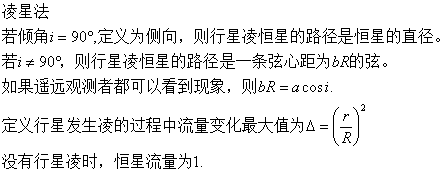
\includegraphics{A_1.png}

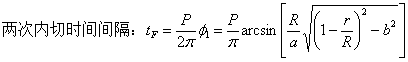
\includegraphics{A_2.png}

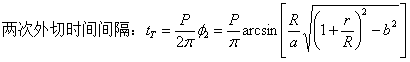
\includegraphics{A_3.png}

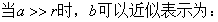
\includegraphics{A_4.png}

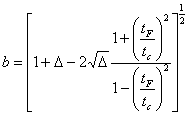
\includegraphics{A_5.png}

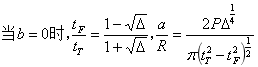
\includegraphics{A_6.png}

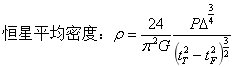
\includegraphics{A_7.png}


\section{变星}
\paragraph{变星的分类}变星是恒星的光度、光谱特征、磁场等物理特性随着时间做周期性的、半规则或无规则变化的恒星。更广义的概念,变星是一切亮度有变化的恒星。
\subparagraph{几何变星(或称作食变星)}双星中一颗较亮,而一颗较暗,双星互相掩食导致亮度呈现周期性变化。

\subparagraph{分光双星}双星的相对运动不明显,但是光谱线由于轨道运动的多普勒效应而呈现周期性变化。

\subparagraph{物理变星}本身物理状态的变化引起光变的变星,称作物理变星。
\paragraph{脉动变星}脉动变星的星体不断产生径向脉动,即交替的膨胀和收缩,从而引起半径、光度、温度乃至磁场发生周期性或者非周期性的变化。在赫罗图上,脉动变星大部分位于主星序上方的一个区域,其中最典型的有造父变星和天琴座RR型星,属于星族\Rmnum{1}。经典的造父变星属于黄色的矩形和超巨星,光变周期多为1至50天,光变幅度大致在0.5至 1.5等,光变曲线相似——亮度在上升时较快而变暗时较慢。在亮度极大时光谱型一般为F型,亮度极小时一般为G或K型。

还有少部分造父变星位于旋涡星系的球状星团和一些椭圆星系中,称作室女座W型星,属于星族\Rmnum{2}。两种造父变星的光变曲线相似,都可以通过周光关系获得其距离。

天琴座RR型变星的光谱型大多为A型,只有一小部分为F型,其绝对星等大致相同为0.6等。

长周期变星的代表为蒭藁增二,光谱型大都属于M型,少数属于N、S、R型。光谱型越晚,周期越长,光度越小。

\paragraph{爆发变星}爆发变星包括:新星、超新星、矮新星、类新星和耀星等。其中,新星和超新星可以作为天体测量的工具。超新星会在本章稍后内容予以详细介绍。

新星在几天之内增亮到9$\sim$14个星等,达到极大时又逐渐减弱,在几个星期内有起伏地下降到爆发之前的状态。新星爆发的时候是恒星演化的晚期,起源于一颗白矮星和一颗巨星组成的密近双星,白矮星吸收巨星的物质达到钱德拉塞卡极限后发生核聚变,抛射大量物质,产生气壳使亮度急剧增加。
\section{星际物质}
\subsection{分子云和恒星形成}
\paragraph{分子云的特征}观测标明,分子云是恒星形成活动的主要场所。巨分子云 包含的质量约为十万倍的太阳质量到六百万倍太阳质量,其大小为几十秒差距。巨分子云其实是复杂体,它由许多小块组成,这些小云块的质量在一千到一万倍的太阳质量之间,尺度2至5秒差距,温度约10开尔文。

分子云物质的主要部分包含在矮分子云内,并不局限于悬臂,可能经历了银河系旋转很多次,寿命为$10^8$年或更长。与之相反的是,含有O、B星的巨分子云的热核心可能当其跨过悬臂时被聚集或解离,时标约为$10^7$年。
\paragraph{暗分子云}
在太阳周围几百秒差距的半径内,有许多消光很大的云。存在的分子云主要是氢气和一氧化碳,后者可以观测到射电波段的谱线。
\paragraph{分子云和年轻恒星在银河系内的分布}
分子云的分布更多集中于$R\sim5.5kpc$(太阳到银心的距离大约为10kpc),范围$\Delta R\sim3kpc$之内,分子云物质大都位于太阳所在圆环之内,且集中于银道面。分子云和中性氢在$R<4kpc$范围内迅速下降,分子云的平均半径厚度大约为60pc,而中性氢为130pc。
\subsection{气体星云在各波段的表现形式}
\paragraph{光学观测}气体云一般称为气体星云,根据光学表现形式可以划分为以下不同的几种:
\subparagraph{暗星云}由背景星或某些其他背景(如H\Rmnum{2}区一样较亮的)遮掩可以观测到。
\subparagraph{反射星云}有镶嵌在云里的散射光可以加以观测,光谱是镶嵌星的发射光线或反射吸收线光谱。
\subsection{H\Rmnum{1}区}根据光学观测,证明在中性氢区内有Na,K,Ca\Rmnum{2},Ti\Rmnum{2},Fe,CN,CH,$CH^+$等原子和分子存在,H\Rmnum{1}区星际云的密度约为每立方米一百万个氢原子,半径为10秒差距,质量约为太阳质量的一千倍,并以每秒10千米的速度做不规则运动。
\subparagraph{H\Rmnum{2}区}围绕着新形成的热而亮的星(O,B型)的亮的电离区。光谱中发射线占据主要地位,也发射连续谱。这些热星发出很强的紫外辐射,比莱曼系限能高的光子和可电离氢原子。H\Rmnum{2}区和H\Rmnum{1}区之间存在着很明显的分界线,中心星发出的紫外光子使得H\Rmnum{2}区的电离和复合达到平衡的部分,称作斯特龙根球。

斯特龙根的假设:恒星变亮的过程很快;周围介质处处均匀。如果中心星发出若干个能使周围气体电离的光子,则相同的时间内原子失去的电子数应该与之相同。设热星周围被春氢所包围,$\dd N_{i}$是单位时间内发自中心恒星的紫外光子数。设光子仅仅电离一个氢原子,$\dd R$为单位时间内单位体积内质子和电子符合为氢原子的个数。在定态情况下,半径为$r$的斯特龙根球内复合的总数应该和电离的总数相平衡:
\begin{equation}
	\dd R\left(\frac{4\pi r^3}{3}\right)=\dd N_{i}
\end{equation}
复合系数$\alpha$是氢等离子体的温度的函数。$\dd R=\alpha n_{p}n_{e}=\alpha n^2_{e}$则:
\begin{equation}
	r=\left(\frac{3dN_{i}}{4\pi\alpha n^2_{e}}\right)^{\frac{1}{3}}
\end{equation}
\subparagraph{行星状星云}类似于H\Rmnum{2}区,但中心天体是演化到晚期的热星,行星状星云比H\Rmnum{2}区更密。
\subparagraph{超新星遗迹}光谱主要是发射线,在年轻的超新星遗迹中,无定形区由同步回旋过程发生连续谱,其射电辐射是非热辐射,但是X射线发射和光学谱线可以由热过程(激波加热气体)产生。
\paragraph{射电观测}射电观测包括连续谱和谱线两类。中性氢波长21厘米的谱线来源氢原子的电子自旋倒转跃迁产生的射电辐射。叫密的中性星际氢云,沿着银河系旋涡结构的悬臂聚集,该分布可能对于H\Rmnum{2}区同样成立。
\paragraph{红外观测}可以期望有H\Rmnum{2}区产生自由-自由跃迁而发出红外连续辐射,但由星际尘埃产生的红外连续辐射更强。
\paragraph{紫外、X射线和$\gamma$射线观测}通过UV波段的观测可以证明密星际云中氢分子是气体氢的主要成分,星际云中重元素的丰度(该元素的密度和总密度的比值),低于星族\Rmnum{1}内恒星重元素的丰度——可以论证星际介质中的重元素大部分被锁到星际尘埃内。

超新星遗迹是重要的X射线源。
\subsection{星际气体的物理过程}
\paragraph{辐射转移}
根据基尔霍夫定律,可以写成:
\begin{equation}
	B_{\nu}(T)=\frac{j_{\nu}}{k\nu}
\end{equation}
在等温条件下,辐射强度可以写成:
\begin{equation}
	I_{\nu}=I_{0}\exp(-\tau)+B_{\nu}(T)(1-e^{-\tau})
\end{equation}
\paragraph{电离和复合}
电离是恒星的电磁能转换为周围星际物质热能的主要方式。电离伴随着复合,这两个过程之间的平衡决定了气体的电离状态(作为恒星光度的函数),观测和理论都指出气体星云的化学丰度多少类似于宇宙丰度,可以说,气体加热主要是氢的光致电离。

当入射光的频率大于电离需要的频率时,基态发生光致电离的截面:
\begin{equation}
	a_{\nu}(K)=\frac{\sigma_{0}}{Z_{K}^2}\left(\frac{\nu_{K}}{\nu}\right)^2
\end{equation}
$\nu_{K}$是阈频率。
电离率表示为:
\begin{equation}
	\frac{1}{\tau_{i}}=\int_{\nu_{1}}^{\infty}\frac{4\pi J_{\nu}(r)}{h\nu}a_{\nu}(H)\dd \nu
\end{equation}
其中,$J_{\nu}(r)$和产生电离的恒星光度有关:(此处$L_{\nu}(r)$不是恒星的光度)
\begin{equation}
	4\pi J_{\nu}(r)=\frac{L_{\nu}(r)}{4\pi r^2}
\end{equation}
如果定义速度为$v$的电子被俘获到原子的态($n=1$称作基态)的截面为$\sigma_{n}(\nu)$,则由复合到态n的复合率:
\begin{equation}
	\frac{1}{\tau_{R}}=\sum_{n=1}^{\infty}\int n_{e}\sigma_{n}(v)vf(v)\dd v=\alpha n_{e}
\end{equation}
其中,$\alpha=\alpha(T_{k})$是复合系数,通过电子的麦克斯韦分布而依赖于电子的温度。复合截面$\sigma_{n}(v)\sim v^{-2}$。

当介质处于稳定状态,光致电离和复合过程的速率相等。考虑中性氢的电离-复合平衡,有:
\begin{equation}
	n(H^0)\int_{\nu_{1}}^{\infty}\frac{4\pi J_{\nu}(r)}{h\nu}\alpha_{\nu}(H^0)\dd \nu=n_{e}n(H^+)\int \dd v\sum_{n=1}^{\infty}vf(v)\sigma_{n}(v)=n_{e}n(H^+)\alpha(H^0)
\end{equation}

在H\Rmnum{2}区和行星状星云中,加热通过光电子,其能量为:
\begin{equation}
	\varepsilon_{n}=\frac{1}{2}m_{e}v^2=h\nu-\chi_{K}=h(\nu-\nu_{K})
\end{equation}
以电子能量加热介质的速率是由电离的光子流、电离截面、中性原子数密度和电子能量的成绩,对所有频率积分而得出。
介质加热率:
\begin{equation}
	\begin{split}
		\Gamma =&0.1n(H^0)\int_{\nu_{1}}^{\infty}\frac{4\pi J_{\nu}(r)}{h\nu}\varepsilon_{e}\alpha_{\nu}(H^0)\dd \nu\\
		&=n(H^+)n_{e}\alpha(H^0)\times\frac{\int_{\nu_{1}}^{\infty}\frac{4\pi J_{\nu}(r)}{h\nu}h(\nu-\nu_{1})\alpha_{\nu}(H^0)\dd \nu}{\int_{\nu_{1}}^{\infty}\frac{4\pi J_{\nu}(r)}{h\nu}\alpha_{\nu}(H^0)\dd \nu}\\
		&=n(H^+)n_{e}\alpha(H^0)h\bar{\nu}\\
	\end{split}
\end{equation}
其中,$h\bar{\nu}$表示电离光子的平均能量,对大部分星云,$h\nu_{1}\gg kT_{e}$。
\paragraph{能量损失机制}
\subparagraph{复合辐射}
每次辐射从气体中移走的能量等于俘获的电子能量。下式给出能量损失率。
\begin{equation}
	\begin{split}
		\varLambda_{R}=&n(H^+)\sum_{n=2}^{\infty}\int_{0}^{\infty}n_{e}\nu\frac{1}{2}m_{e}v^2\sigma_{n}(v)f(v)\dd v\\
		=&n(H^+)n_{e}\beta^\prime(H^0)kT_{e}
	\end{split}
\end{equation}
纯复合产生的冷却率:
\begin{equation}
	\begin{split}
		\varLambda_{R}=&\varLambda_{R}(H^+)+\sum\varLambda_{R}(X_{K}^{i})\\
		=&\varLambda_{R}(H^+)\left[1+\sum\frac{n(X_{k}^{i})\beta^\prime(X_{k}^{i})}{n(H^+)\beta^\prime(H^0)}\right]
	\end{split}
\end{equation}
\subparagraph{碰撞激发}
考虑一个典型的电子-离子碰撞,结果实得离子由态$i$激发到态$j$,该过程的激发截面通过下式给出:
\begin{equation}
	\sigma_{ij}=\frac{\pi\hbar}{m_{e}v^2}\frac{\Omega_{ij}}{g_{i}}
\end{equation}
此处,$v$是电子的速度,$g_{i}$为离子的初态的统计权重,$\Omega_{ij}$称作碰撞强度,对于星云通常接近于1。

由速度$v$的电子引起由能级$j$到能级$i$的碰撞去激发的速率应该由电子流、位于激发态$j$的靶离子数密度$n(X_{k}^{i})$,和去激发截面的乘积加以描述;下式给出单位体积的碰撞去激发的速率。
\begin{equation}
	n_{e}n(X_{k}^{i})r_{ij}=n(X_{k}^j)\int_{0}^{\infty}n_{e}v\sigma_{ji}(v)f(v)\dd v
\end{equation}
电子的速度分布是麦克斯韦速度分布。设$\Omega_{ij}$为一常量,可发现去激发速率为:
\begin{equation}
	n_{e}n(X_{k}^{i})r_{ji}=n_{e}n(X_{k}^{i})\left(\frac{2\pi}{kT_{e}}\right)^{\frac{1}{2}}\frac{\hbar^2}{m_{e}^{\frac{3}{2}}}\frac{\Omega_{ji}}{g_{i}}
\end{equation}
可以证明碰撞激发速率由下式给出:
\begin{equation}
	r_{ij}=\frac{g_{i}}{g_{j}}\exp(-\frac{X_{ji}}{kT_{e}})
\end{equation}
其中:
\begin{equation}
	X_{ji}=\frac{m_{e}\left(v_{j}^2-v_{i}^2\right)}{2}
\end{equation}
对于多能级的禁戒跃迁,可以得出以下关系式:
\begin{equation}
	\varLambda_{c,K}=\sum_{i}(X_{K}^{i})\sum_{j>i}A_{ji}h\nu_{ji}
\end{equation}
\subparagraph{韧致辐射}当热电子被气体中离子散射时发射连续谱,发射的能量大都在设点和红外波段,并从星云中逃逸出去。对离子数密度为$n_{e}$,该损失率为:
\begin{equation}
	\varLambda_{ff}=\frac{2^5e^6\pi Z^2}{3^{\frac{3}{2}}hm_{e}c^3}\left(\frac{2\pi k T_{e}}{m_{e}}\right)^{\frac{1}{2}}
\end{equation}
\subsection{星际尘埃}
\paragraph{尘埃的光学特性}
当光经过光深为$\tau_{\lambda}$时后,其观测的辐射强度写成:
\begin{equation}
	I_{\lambda}=I_{\lambda}(0)e^{-\tau_{\lambda}}
\end{equation}
同一光谱型的星在天空不同位置的观测标明,消光和波长的倒数成线性关系,此关系对于紫外到红外波段近似成立。星际介质中原子和分子对于散射的作用可以忽略,因为它和波长的负四次方成正比;类似的,电子的散射也和波长无关。

星际消光与尘埃的数密度为$n_{d}$,半径为$r_{d}$的尘埃球形结构的截面:
\begin{equation}
	\sigma_{d}=\pi r_{d}^2
\end{equation}
包括散射和吸收的体消光系数通常表示为:
\begin{equation}
	\kappa_{ex}=n_{d}Q_{e}(\lambda)\sigma_{d}
\end{equation}
和波长有关的量$Q_{e}(\lambda)$确定了截面为$\sigma_{d}$的尘埃对星光减弱的效率,以尘埃柱密度为$n_{d}$,可以写出:
\begin{equation}
	\tau_{\lambda}=\int \kappa \dd r=Q_{e}(\lambda)\sigma_{d}n_{d}
\end{equation}
消光一般以星等为$A_{\lambda}=m-m_{0}$,此处$m_{0}$表示没有尘埃时沿视线的视星等。利用星等和光度的关系,则得到:
\begin{equation}
	A_{\lambda}=-2.5\log\frac{I_{\lambda}}{I_{\lambda}(0)}
\end{equation}
由尘埃对星光的散射或吸收后,再经由尘埃发出辐射,此时在旋涡星系的盘面内产生弥漫背景辐射。定义在$\Omega^\prime$方向传播的星光强度为$I_{\lambda}(\Omega\prime)$,则尘埃散射到方向为$\Omega$的立体角的光的强度为$I_{\nu}(\Omega^\prime)Q_{s}\sigma_{d}$,此处尘埃的散射效率$Q_{s}$。如果辐射强度为$I_{\nu}(\Omega^\prime)$的光被散射到$\Omega$方向的部分为$F(\Omega,\Omega^\prime)$,那么发射系数为:
\begin{equation}
	j_{\nu,s}=Q_{s}\sigma_{d}n_{d}\int I_{\nu}(\Omega^\prime)F(\Omega,\Omega^\prime)\dd \Omega^\prime
\end{equation}
对这一散射发射系数还需要加上尘埃的热发射系数$j_{\nu,T}$。引入吸收率$Q_{a}=Q_{e}-Q_{s}$,以$T_{d}$表示尘埃的温度,于是它的辐射可以作为黑体辐射且处于局部热动平衡,根据基尔霍夫定律可得:
\begin{equation}
	j_{\nu,r}=\kappa_{\nu}^{a}B_{\nu}(T_{d})
\end{equation}
吸收系数为:
\begin{equation}
	\kappa_{\nu}^{a}=n_{d}Q_{a}\sigma_{d}
\end{equation}
对于$\lambda>2\pi r_{d}^2$,$Q_{a}$近似于1。对于$\lambda\leq 2\pi r_{d}^2$,$Q_{a}$小于1。但对于铁球,峰值为2然后渐渐趋近于1。
\paragraph{尘埃的物理特性}
尘埃的加热有三条途径。第一条是尘埃来吸收来自恒星的弥漫光子的辐射加热,局部辐射场的能量密度由普朗克定律给出,单位时间入射到尘埃单位面积的能量$cu_{\lambda}$,乘吸收效率$Q_{a}$,并对整个波长积分则给出:
\begin{equation}
	\varGamma_{R}=c\int_{0}^{\infty}u_{\lambda}Q_{a}(\lambda)\dd \lambda
\end{equation}
第二个加热机制是尘埃和分子作非弹性碰撞时原子和分子的动能传给尘埃。第$K$种元素以速度$v_{K}$运动的分子和押金自的动能变化为:
\begin{equation}
	E_{K}=\frac{1}{2}m_{K}v_{K}^2-\bar{E}_{K}
\end{equation}
$\bar{E}_{K}$是原子的平均反弹动能。尘埃获能率由能流$n_{K}v_{K}\Delta E_{K}$,对麦克斯韦速度分布函数取平均,并对各种组成取和得到:
\begin{equation}
	\varGamma_{c}=\sum_{K}n_{K}\int f_{K}(v)\dd v_{K}\Delta E_{K}v_{K}
\end{equation}
在尘埃表面将增强分子形成,复杂分子的大部分在尘埃表面形成。当两个原子,或者一个原子和一个简单分子相结合,他们束缚能的相当部分储存在尘埃上。与之相应的加热率可以表示为:
\begin{equation}
	\varGamma_{B}=\sum_{K}\xi_{K}\eta_{K}\int f(v_{K})\dd v_{K} \eta_{K}E_{B,K}v_{K}
\end{equation}
尘埃的总加热率:
\begin{equation}
	\varLambda_{R}=\varGamma_{B}+\varGamma_{c}+\varGamma_{R}
\end{equation}
令稀释因子$W$,可以得到尘埃的温度为:

\begin{equation}
	T_{D}=T_{e}W^{\frac{1}{5}}
\end{equation}

以下考虑电子的光致抛射。类似于金属中的光电效应 。为了从中性尘埃中移走一个电子,电子必须具有足够的能量用以克服其束缚在尘埃表面的束缚能。若以$h\nu_{c}$表示这个能量,只有比这个能量高的光子才能产生自由电子。若尘埃带负电$Z_{d}<0$,电子抛射的阈值能量同样为$h\nu_{c}$。反之,电子需要克服的能量需要加上克服的静电势能。
\begin{equation}
		h\nu_{z}=\left\{
	\begin{aligned}
		h\nu_{c} \quad Z_{d}\leq 0\\
		h\nu_{c}+\frac{Z_{d}e^2}{ah} \quad Z_{d}>0	\\
	\end{aligned}
		\right
		.
\end{equation}
$\varphi_{\nu}$表示尘埃吸收一个能量$h\nu$并抛射一个电子的概率。尘埃电荷变化由下式给出:
\begin{equation}
	\frac{\dd Z_{d}}{\dd t}=\pi a^2\int_{\nu_{z}}^{\infty}\frac{4\pi J_{\nu}}{h\nu}\varphi_{\nu}\dd \nu
\end{equation}
对于带负电的尘埃,这个速率和$Z_{d}$没有关系。电子和离子对尘埃碰撞对$Z_{d}$也有贡献。由能量守恒定律和角动量守恒定律联立可初始速度为$v_{i}$的离子被俘后的有效截面:
\begin{equation}
	\pi a_{c}^2=\pi a^2\left(1-\frac{2Z_{i}eU}{m_{i}v_{i}^2}\right)
\end{equation}
其中,尘埃的静电电势:
\begin{equation}
	U=\frac{Z_{d}e}{a}
\end{equation}
在电离氢区和行星状星云中由于俘获质子,尘埃的电荷增加率可以由离子流乘截面再对离子的速度分布积分得到:
\begin{equation}
	\left(\frac{\dd Z_{d}}{\dd t}\right)_{p}=\xi_{p}\int_{v_{min}}^{\infty}n_{p}\pi a_{c}^2vf(v)\dd v
\end{equation}
$\xi_{p}$是碰撞粒子实际上粘在尘埃上的概率。
当电荷和尘埃粒子相碰:
\begin{equation}
	\left(\frac{\dd Z_{d}}{\dd t}\right)_{p}=\left\{
\begin{aligned}
		n_{p}\pi a^2\xi_{p}\left(\frac{8kT}{\pi m_{H}}\right)^{\frac{1}{2}}\exp(-\frac{Z_{d}e^2}{akT})\quad Z_{d}>0\\
		n_{p}\pi a^2\xi_{p}\left(\frac{8kT}{\pi m_{H}}\right)^{\frac{1}{2}}\left(1-\frac{Z_{d}e^2}{akT}\right)\quad Z_{d}\leq 0\\
\end{aligned}
	\right
	.
\end{equation}
当电子和尘埃相碰时,电荷增加率:
\begin{equation}
	\left(\frac{\dd Z_{d}}{\dd t}\right)_{p}=\left\{
	\begin{aligned}
		-n_{e}\pi a^2\xi_{e}\left(\frac{8kT}{\pi m_{e}}\right)^{\frac{1}{2}}\left(1+\frac{Z_{d}e^2}{akT}\right)\quad Z_{d}>0\\
		-n_{e}\pi a^2\xi_{e}\left(\frac{8kT}{\pi m_{e}}\right)^{\frac{1}{2}}\exp(\frac{Z_{d}e^2}{akT})\quad Z_{d}\leq 0\\
	\end{aligned}
	\right
	.
\end{equation}
$\xi_{e}$是电子碰到尘埃时实际被粘在尘埃上的概率。对于稳定态,电荷量被确定,有:
\begin{equation}
	\left(\frac{\dd Z_{d}}{\dd t}\right)=\left(\frac{\dd Z_{d}}{\dd t}\right)_{e}+\left(\frac{\dd Z_{d}}{\dd t}\right)_{p}+\left(\frac{\dd Z_{d}}{\dd t}\right)_{light}=0
\end{equation}
忽略光致作用,有:
\begin{equation}
	\left(\frac{n_{e}}{n_{p}}\right)\exp(\frac{Z_{d}e^2}{akT})=\left(\frac{m_{p}}{m_{e}}\right)^{\frac{1}{2}}\left(1-\frac{Z_{d}e^2}{akT}\right)
\end{equation}
\subsection{星际气体动力学过程}
\paragraph{星际空间中的激波}
当气体的运动超过声速时,必然形成激波。

\noindent 质量守恒得连续性方程:
\begin{equation}
	\frac{\partial \rho}{\partial t}+u\frac{\partial \rho}{\partial x}+\rho\frac{\partial u}{\partial x}=0
\end{equation}
动量守恒得到运动方程:
\begin{equation}
	\frac{\partial u}{\partial t}+u\frac{\partial u}{\partial x}=-\frac{1}{\rho}\frac{\partial P}{\partial x}
\end{equation}
能量守恒得到能量方程:
\begin{equation}
	\frac{\dd \varepsilon}{\dd t}+P\frac{\dd v}{\dd t}=Q
\end{equation}
此处比容$v=1/\rho$,气体的宏观速度为$u$。

借助连续性方程和运动方程可以写出:
\begin{equation}
	\frac{\partial}{\partial t}\left(\rho\varepsilon +\frac{\rho u^2}{2}\right)=-\div \left[\rho u\left(\varepsilon+\frac{u^2}{2}\right)+Pu\right]+\rho Q
\end{equation}
质量守恒:
\begin{equation}
	\rho_{0}u_{0}=\rho_{1}u_{1}=\varphi
\end{equation}
以下三个量在激波面前后是守恒的:
质量流:
\begin{equation}
	\varphi=\rho u
\end{equation}
动量流:
\begin{equation}
	\zeta=P+\rho u^2
\end{equation}
总比能量(单位质量物质的总能量):
\begin{equation}
	\xi =\frac{1}{2}u^2+\frac{5}{2}\frac{P}{\rho}
\end{equation}
如果气体遵从绝热物态方程,那么局部声速可以写成:
\begin{equation}
	a^2=\frac{5}{3}\frac{P}{\rho}
\end{equation}
马赫数可以表示为:
\begin{equation}
	M=\frac{u^2}{\frac{5}{3}\frac{P}{\rho}}=\frac{3}{5}\frac{u}{\bar{u}-u}
\end{equation}
其中参考速度$\bar{u}$定义为:
\begin{equation}
	\bar{u}=\frac{\zeta}{\varphi}
\end{equation}
引入变量:$\eta=u/\bar{u}$,可以写出比总能、比内能、比动能、马赫数分别为:
\begin{equation}
	\varepsilon_{T}=\frac{\xi}{\bar{u}^2}=\eta\left(\frac{5}{2}-2\eta\right)
\end{equation}
\begin{equation}
	\varepsilon_{1}=\frac{e}{\bar{u}^2}=\frac{3}{2}\eta\left(1-\eta\right)
\end{equation}
\begin{equation}
	\varepsilon_{K}=\frac{1}{2}\eta^2
\end{equation}
\begin{equation}
	M^2=\frac{3}{5}\frac{\eta}{1-\eta}
\end{equation}

将动量守恒方程写成:
\begin{equation}
	u^2-\bar{u}u+\frac{3}{5}a^2=0
\end{equation}
或者写成:
\begin{equation}
	u^2-\frac{5}{4}u\bar{u}+\frac{1}{2}\xi=0
\end{equation}
该方程有两个根,分别是逆流和顺流的速度。逆流的马赫数:
\begin{equation}
	M_{0}^2=\left(\frac{u_{0}}{a_{0}}\right)^2=\frac{3}{5}\frac{u_{0}}{\bar{u}-u}
\end{equation}
对于强激波,逆流的马赫数远大于1。
\begin{equation}
	\frac{u_{1}}{u_{0}}=\frac{M_{0}+3}{4M_{0}^2}=\frac{1}{4}
\end{equation}
有的时候可以写成:
\begin{equation}
	u_{0}-u_{1}=\frac{3}{4}u_{0}
\end{equation}
利用连续性方程和质量守恒得到:
\begin{equation}
	\rho_{1}=4\rho_{0}
\end{equation}
因为跨过激波的压强变化十分大,可以忽略$P_{0}$,得到:
\begin{equation}
	P_{1}=\rho_{0}u_{0}^2-\rho_{1}u_{1}^2=\frac{3}{4}\rho_{0}u_{0}^2
\end{equation}
结合理想气体的状态方程,得到激波后的温度:
\begin{equation}
	T_{1}=\frac{3}{16}\frac{\mu m}{k}u_{0}^2=\frac{\mu m\left(u_{0}-u_{1}\right)^2}{3k}
\end{equation}
对于参考系的变化,假设在某固定的参考系中,激波的速度为$v_{s}$,逆流速度和顺流速度分别为$U_{0}$和$U_{1}$。存在变换:
\begin{equation}
	u_{0}=U_{0}-v_{s}\qquad u_{1}=U_{1}-v_{S}
\end{equation}
通常$v_{s} \gg U_{0}$,变换后得到的有关关系式:
\begin{equation}
	\frac{v_{s}-U_{1}}{v_{s}}=\frac{1}{4}\qquad U_{1}=\frac{3}{4}v_{s}
\end{equation}
\begin{equation}
	P_{1}=\frac{3}{4}\rho_{0}v_{s}^2
\end{equation}
\begin{equation}
	T_{1}=\frac{3\mu m}{16k^2}v_{s}^2
\end{equation}
\begin{equation}
	e_{1}=\frac{3}{2}\frac{P_{1}}{\rho_{1}}=\frac{9}{32}v_{s}^2\rho_{0}\qquad e_{K}=\frac{1}{2}U_{1}^2=\frac{9}{32}v_{s}^2\rho_{0}
\end{equation}
\paragraph{星云的运动}
\subparagraph{光致电离星云}氢组成的均匀星云中某处形成了一颗大质量恒星,经过较短的时间(十万年以内),该大质量年轻恒星达到稳定,并维持越三百万年。电离气体球的半径是时间的函数,电离气体球和中性气体之间的界面称作电离波前,简称I-F。该区域的厚度远小于电离区的尺度,可以看做平行平面结构。

在相对恒星静止的参考系中,围绕恒星的气体是静止的。I-F在$t$时,相对恒星的距离为$R$;在$t+\dd t$时,距离为$R+\dd R$。假设$J$是每秒垂直落到I-F单位面积上的莱曼连续光子数,在I-F内部是完全电离的。考虑I-F的单位面积,必然有:
\begin{equation}
	\frac{\dd R}{\dd t}=\frac{J}{n_{0}}
\end{equation}
假设$S_{*}$是单位时间内从I-F释放出的光子和中性气体复合的次数,则:
\begin{equation}
	S_{*}=4\pi R^2J+\frac{4}{3}\pi R^3n_{0}^2\beta_{2}
\end{equation}
此处,$\beta_{2}$为复合系数,于是:
\begin{equation}
	J=\frac{S_{*}}{4\pi R^2}-\frac{1}{3}Rn_{0}\beta_{2}
\end{equation}
斯特龙根球的半径:
\begin{equation}
	R_{s}=\left(\frac{3}{4\pi}\frac{S_{*}}{n_{0}^2\beta_{2}}\right)
\end{equation}
和氢的复合相对应的时间为:
\begin{equation}
	t_{R}=\frac{1}{n_{0}\beta_{2}}
\end{equation}
\begin{equation}
	\frac{R}{R_{s}}=\left[1-\exp(\frac{t}{t_{R}})\right]^{\frac{1}{3}}
\end{equation}
通常计算时所用数值:
$S_{*}=10^{49}s^{-1}$,$\beta_{2}=2\times 10^{-19}m^3\cdot s$,$t_{R}=5\times 10^{18}n_{0}^{-1}s$,$R_{s}=2\times 10^{22}n_{0}^{-\frac{2}{3}} m$,
$v_{R}\sim 4\times n_{0}^{\frac{1}{3}}$,
$n_{0}=10^{18}m^{-3}$
\subparagraph{星风对星际气体的影响}
由观测非常亮的热星的光谱可知,这些星从表面连续地抛射物质而损失质量。这种质量的损失称作星风。星风以机械能输出的功率为$10^{29}W$量级,因为紫外光子转化为气体动能的效率很低,所以紫外光子的输出效率会比机械能输出功率再高几个数量级。星风以告诉推动星际气体,该速度显然超过了声速。星风在星际气体生成激波。从靠近恒星到远离恒星,星风共有三个界面($S_{1}$,C,$S_{2}$),和四个区(从内到外为a,b,c,d)。

区域a是由速度$v_{*}\sim2000km/s$的未产生激波的星风所占据,当它进入激波$S_{1}$,激波转化星风的部分能量成为热能。

区域b是包含激波的星风气体。该激波的马赫数很高,激波很强,激波后的气体的温度$T\sim 4\times 10^7K$。

区域c是激波$S_{2}$通过的气壳,在该区域辐射冷却很有效。该区域很薄,在$S_{1}$和$S_{2}$之间具有均匀的压强。界面C是间断面,将产生激波的星风和产生激波的星际气体分开。穿过该界面,气体的温度、密度等物理量发生间断,这意味着没有物质流跨过此界面。

区域d是周围的电离气体。作为近似,可以认为它们是静止的。
\subparagraph{超新星爆发对星际介质的影响}
设在密度为$n_{0}$的均匀星际介质中某一点突然释放很大能量$E_{*}\sim10^{43}\sim10^{44}J$。这些能量的沉积导致靠近爆发星的星际气体加热,温度和压力都变得很高,于是膨胀。如果忽略星际气体的电离状态,膨胀速度超过声速。于是形成激波并传向星际介质,且扫过星际气体。设此激波$S$的半径为$R$,运动速度为$\dot{R}$,激波初始速度很高,但气泡膨胀时此速度便下降。

$\left(1\right)$超新星爆发后形成的膨胀气泡的半径和运动速度——这一阶段称作能量守恒阶段。

强激波前后的单位质量动能和热能相等且由下式给出:
\begin{equation}
	e_{T}=e_{K}=\frac{9}{32}\dot{R}^2
\end{equation}

激波的速度即为半径对时间的导数。因为激波前的气体认为是静止的,假设膨胀泡的密度为$\rho_{0}$,其内气体的总能量为:
\begin{equation}
	E_{T}=\frac{4}{3}\pi R^3\rho_{0}(e_{T}+e_{K})=\frac{3}{4}\pi n_{0}m_{H}R^3\dot{R}=E_{*}
\end{equation}
膨胀泡的边界的运动方程式:
\begin{equation}
	R^3\dot{R}^2=\frac{4}{3\pi}\frac{E_{*}}{\rho_{0}}
\end{equation}
认为激波球的半径从零开始变化的时刻为计时原点,作为边界条件,有:
\begin{equation}
	\dot{R}=\left(\frac{25}{3\pi}\right)^{\frac{1}{3}}\left(\frac{E_{*}}{\rho_{0}}\right)^{\frac{1}{5}}t^{\frac{2}{5}}
\end{equation}
可以进一步得出,超新星遗迹的半径和速度的关系:
\begin{equation}
	R=\frac{5}{2}v_{*}t
\end{equation}

$\left(2\right)$超新星遗迹(SNR)的壳层半径和运动速度——动量守恒阶段。
当辐射能大于超新星爆发初始能量的一般时,超新星遗迹进入该阶段。

根据动量守恒定律,下式成立:
\begin{equation}
	\frac{4}{3}\pi R^3\rho_{0}\dot{R}=\mu_{0}=const
\end{equation}
假设该壳层是在时间为$t_{0}$时瞬时形成的,当$R=R_{0}$,有$\dot{R}=\dot{R}_{0}$,对上式积分得到:
\begin{equation}
	R=R_{0}\left[1+4\frac{\dot{R}_{0}}{R_{0}}\left(t-t_{0}\right)\right]^{\frac{1}{4}}
\end{equation}
\begin{equation}
	\dot{R}=\dot{R}_{0}\left[1+4\frac{\dot{R}_{0}}{R_{0}}\left(t-t_{0}\right)\right]^{-\frac{3}{4}}
\end{equation}
对于足够长的时间,$R\sim t^{\frac{1}{4}}$,$\dot{R}\sim t^{-\frac{3}{4}}$,这是动量守恒的特征。和能量守恒的阶段相比,$R\sim t^{\frac{2}{5}}$,$\dot{R}\sim t^{-\frac{3}{5}}$
\subsection{恒星和星际物质之间的相互作用}
\paragraph{恒星的死亡}
对于晚型的巨星和超巨星,质量流中往往伴随着尘埃。形成何种尘埃可能取决于恒星大气中的碳和氧是否相对更丰富。碳和氧试图结合成为稳定的一氧化碳。一旦该过程完成,它们就同其他元素的原子或它本身的原子形成分子。某些这些分子,例如含有硅的成分,可以凝结成小的颗粒。

尘埃颗粒可以再新星爆发的气壳中形成,也可以在行星状星云中形成。超新星爆发的抛射中可以形成含有某些丰富元素的同位素的尘埃。

超新星爆发可以对周围星际介质提供动量;原来爆发时的许多动能转化为热能,又在激波后薄的壳层中以辐射形式逐渐释放掉。因此,此阶段超新星加速星际介质的效率并不高。
\paragraph{恒星的诞生}
一颗亮而热的恒星突然出现在中性氢云和电离氢气体云中,必然对该系统产生比较大的影响。靠近这颗星的密的氢气将完全被电离,形成致密的电离氢区。该电离氢区的气体因为被加热而膨胀,开始运动。在巨分子云复杂体中,低质量的恒星也在形成。如,金牛座T型星,具有以下特点:

$\left(1\right)$镶嵌在密的气体的尘埃中,发现T Tau星的暗星云中往往包含着特殊的亮星云——被认为是收缩中的原恒星的阿罗-赫比格天体。

$\left(2\right)$光谱通常有强烈的发射线,该性质可以认为它存在强烈的色球活动。

$\left(3\right)$光谱可以证明存在很强的恒星风,同样可以反映强烈的色球活动。

$\left(4\right)$亮度可以再几个小时内反复无常地变化,原因不详。

$\left(5\right)$大气中含有大量的锂元素,证明该星有表层活动。

根据位力定理,对形成平衡的系统,有:
\begin{equation}
	2U+W=4\pi r^3P_{out}
\end{equation}
对于等温非简并的气体,$U=1.5NkT$,若气体的摩尔质量为$m$,有:
\begin{equation}
	P_{out}=\frac{MkT}{mV}-\frac{\beta GM^2}{V^{\frac{4}{3}}}
\end{equation}
此处使用了\begin{large}
	$\beta =\left(\frac{4\pi}{3}\right)^{\frac{1}{3}}\frac{\alpha}{3}$
\end{large}
定义无量纲量的体积和压力如下:

\begin{large}
	$v=\frac{V}{\left(\frac{GMm}{kT}\right)^3}$ \qquad $p=P_{out}\frac{G^3M^2}{\left(\frac{m}{kT}\right)^4}$
\end{large}

可以证明,
\begin{equation}
	P=\frac{1}{v}-\frac{\beta}{v^{\frac{4}{3}}}
\end{equation}
可以求出$P_{out}$和$V$的临界值。
气体中心密区的动力学坍缩过程往往进行得很快。在很多情况下,密的中心区下落形成不透明的核。核的下落在强激波中加以制动,经过某些过程之后,在气团中心形成一达到流体静力学平衡的天体,称作原恒星。该原恒星的初始质量可能只有太阳质量的千分之一,但它吸积它周围的气体和星核落到它之上的时标为一万到一百万年,这取决于触发坍缩的具体条件。一个理想的球形坍缩问题从内到外的性质:
$\left(1\right)$流体静力学的核,原恒星。

$\left(2\right)$一辐射激波,决定了核的表面和下落到表面的物质流并加以制止。

$\left(3\right)$无尘埃区,来自辐射激波向外传播的光子加热气体到高温,从而使尘埃被破坏。

$\left(4\right)$一个由下落物质组成的不透明的尘埃壳层,将向外传输的光子转化为红外光子。

$\left(5\right)$一个充满尘埃的伪光球,在此处红外光子已经衰减为长波。

在原恒星的吸积阶段,中心原恒星在光学波段不可见;充满尘埃的伪光球在红外波段可见;对于足够热而亮的中心恒星,无尘埃区外有一完全电离并在射电波段课件的电离氢区。
\section{恒星的形成与早期演化}
\subsection{恒星演化的四个时标}
\paragraph{自由下落时标}恒星的自由下落时标取决于引力场的强度和所含物理量的量纲,所需的时间唯一地由恒星的质量$M$,半径$R$和引力常量$G$表示为:
\begin{equation}
	t=\left(\frac{R^3}{GM}\right)^{\frac{1}{2}}
\end{equation}
处于稳定状态的恒星能够很快调整自身压力-引力的不平衡,处于流体静力学平衡状态。
\paragraph{开尔文-亥姆霍兹(K-H)时标}恒星演化的进程主要由能源决定,当恒星收缩释放出的引力势能能够完全供给恒星产生的能量的时间称作开尔文-亥姆霍兹时标:
\begin{equation}
	t_{K}=\frac{\frac{GM}{R^2}}{L}
\end{equation}
\paragraph{爱因斯坦时标}爱因斯坦时标是恒星全部质能(根据质能方程给出)完全转化为辐射能的时间。
\begin{equation}
	t_{n}\sim\frac{Mc^2}{L}
\end{equation}
\subsection{物质凝聚和恒星形成}
合理估计得出主序星的寿命:
\begin{equation}
	\tau\approx\frac{M}{M_{sun}}\frac{L}{L_{sun}}\times 10^10 \quad a
\end{equation}

\subsection{金斯判据}
假设星云的半径为$r$,质量为$M$,则一个位于星云边缘的气体粒子加速度近似为:
\begin{equation}
	\frac{r}{\tau_{ff}^2}\sim\frac{GM}{r^2}\sim\frac{4\pi}{3}G\bar{\rho}r
\end{equation}
其中,气体星云的平均密度为$\bar{\rho}$,得到自由下落时标写成:
\begin{equation}
	\tau_{ff}\sim\sqrt{\frac{4\pi}{3}G\bar{\rho}}
\end{equation}
\paragraph{动力学方程线性化}
对于温度和密度都不太高(非相对论情形)的星云(视作流体),不考虑磁场。设其有关的物理量为质量密度$\rho$
\begin{equation}
	\rho\frac{\dd \boldsymbol{v}}{\dd t}=\boldsymbol{f}-\nabla P
\end{equation}
\begin{equation}
	\frac{\partial \rho}{\partial t}+\nabla(\rho\boldsymbol{v})=0
\end{equation}
\begin{equation}
	\nabla^2\varphi=4\pi G \rho
\end{equation}
\begin{equation}
	\nabla\times (\boldsymbol{v}\times \boldsymbol{B})=\frac{\partial B}{\partial t}-\frac{1}{4\pi\sigma}(\boldsymbol{B}\cdot\nabla)\boldsymbol{B}
\end{equation}
以上四个方程已经引入磁场和引力。$\boldsymbol{f}$由下式给出:
\begin{equation}
	\boldsymbol{f}=-\rho\nabla\varphi-\frac{1}{8\pi}\nabla\boldsymbol{B}^2+\frac{1}{4\pi}(\boldsymbol{B}\cdot\nabla)\boldsymbol{B}
\end{equation}
对于各物理量,写为形如$\rho=\rho_{0}+\lambda\rho_{1}$的形式(其实是无穷级数展开并将含有$\lambda^2$及更高次的项删除),代入得到有关物理量相应于$n=1$的线性化方程,泊松方程变为:
\begin{equation}
	\nabla^2\varphi_{0}+\lambda\nabla^2\varphi_{1}=4\pi G\rho_{0}+4\pi G\lambda\rho_{1} 
\end{equation}
但是,$\nabla^2\varphi_{0}=4\pi G\rho_{0}$,有:
\begin{equation}
	\nabla^2\varphi_{1}=4\pi G\lambda\rho_{1} 
\end{equation}
连续性方程化为:
\begin{equation}
	\frac{\partial \rho_{1}}{\partial t}+\nabla(\rho_{0}\boldsymbol{v}_{1}+\rho_{1}\boldsymbol{v}_{0})
\end{equation}
动力学方程化为:
\begin{equation}
	\nabla\times(\boldsymbol{v}_{0}\times \boldsymbol{B}_{1})+(\boldsymbol{v}_{1}\times \boldsymbol{B}_{0})=\frac{\partial \boldsymbol{B}_{1}}{\partial t}-\frac{1}{4\pi\sigma}\nabla^2\boldsymbol{B}_{1}
\end{equation}
此处认为电导率是常数。在线性化条件下,运动方程变为:
\begin{equation}
	\frac{\partial \boldsymbol{v}_{1}}{\partial t}+\boldsymbol{v}_{0}\cdot\nabla\boldsymbol{v}_{1}+\boldsymbol{v}_{1}\cdot\nabla\boldsymbol{v}_{0}=-\nabla\left(\varphi_{1}+\frac{P_{1}}{\rho_{0}}\right)-\frac{\nabla\boldsymbol{B}^2_{1}}{8\pi\rho_{0}}+\frac{(\boldsymbol{B}_{1}\cdot\nabla)\boldsymbol{B}_{0}}{4\pi\rho_{0}}
\end{equation}
当运动是绝热的时候,$P_{1}=\rho_{1}C_{s}^2$,$C_{s}$为声速。
\paragraph{金斯模型}
在无扰动的情况下,满足如下状态:$\rho_{0}=const$,$\boldsymbol{v}_{0}=0$,$\boldsymbol{B}_{0}=0$
经整理得到波动方程:
\begin{equation}
	\left(\nabla^2-\frac{1}{C_{s}^2}\frac{\partial}{\partial t}+\frac{4\pi G \rho_{0}}{C_{s}^2}\right)\rho_{1}=0
\end{equation}
根据波动方程的形式可知,其解为:
\begin{equation}
	\rho_{1}=A\exp\left[i(kr-\omega t)\right]
\end{equation}
这是波矢为$\boldsymbol{k}$和频率为$\omega$的波动。

色散关系满足:
\begin{equation}
	\omega^2=k^2C_{s}^2-4\pi G\rho_{0}
\end{equation}
临界稳定下,$\omega=0$;稳定区域的$\omega^2>0$。得出临界波矢为:
\begin{equation}
	k_{J}=\frac{4\pi G\rho_{0}}{C_{s}^2}=\frac{4\pi G\mu m_{H}\rho_{0}}{kT}
\end{equation}
引入特征线尺度:
\begin{equation}
	l_{J}=\frac{2\pi}{k_{J}}=\sqrt{\frac{\pi}{G\rho_{0}}}C_{s}
\end{equation}
当$k<k_{J}$或$l>l_{J}$时,不稳定。$k_{J}$称作金斯长度。
对于盘形,在特征长度$l_{J}$内的物质可以收缩。
\subsection{旋转的影响}
考虑到星云或银道面上的物质是旋转的,这种情况最简单的假设是认为引力场变弱。星云密度的限制可以表示为(论证从略):
\begin{equation}
	\rho>\frac{3\omega^2}{4\pi G}=\rho_{limit}
\end{equation}
如果密度大于临界密度,由于不稳定性,星云仍然能够坍缩。
\subsection{孤立星云的坍缩}
考虑一个温度为$T^\prime$,密度为$\rho^\prime$的大星云,在其内部有一温度$T$,密度$\rho$,半径为$R$的球体。星云等温、不旋转、无磁场。同时假设$\rho^\prime \ll \rho$,$T^\prime \gg T$。
根据位力定理得到:
\begin{equation}
	3(\gamma-1)U+\Omega-4\pi R^2P_{out}=0
\end{equation}
其中,$\Omega$为引力势能。认为星云的初始状态服从理想气体物态,$\gamma =\frac{5}{3}$
\begin{equation}
	\Omega=-\frac{3}{5}\frac{M^2G}{R}
\end{equation}
如果密度是均匀的,则:
\begin{equation}
	\rho_{c}=\frac{3M_{c}}{4\pi R^3}
\end{equation}
内能:
\begin{equation}
	U=-\frac{2MkT}{3\mu m_{H}}
\end{equation}
中性氢气体的温度一般为50至100开尔文。结合以上假设,位力定理表示为:
\begin{equation}
	P_{out}=\frac{3kTM}{4\pi \mu m_{H}R^3}-\frac{3}{20\pi}\frac{M^2G}{R^4}
\end{equation}
对于一定质量且进行等温收缩的云,达到最大值的半径为:
\begin{equation}
	R_{J}=\sqrt{\frac{3}{\pi}\frac{15}{16}\frac{kT}{\mu m_{H}\rho G}}
\end{equation}
总能量:
\begin{equation}
	E=U+\Omega=\frac{2MkT}{3\mu m_{H}}-\frac{3}{5}\frac{M^2G}{R}
\end{equation}
当总能量为零时,$P_{out}$最大值为:
\begin{equation}
	P_{out}=\pi\frac{\frac{kT}{\mu m_{H}}}{M^2G^3}
\end{equation}
若周围物质的压力大于此值,星云必然坍缩,位力定理改写为:
\begin{equation}
	\frac{1}{2}\frac{\dd^2 I}{\dd^2 t}=3(\gamma-1)U+\Omega-4\pi R^2P_{out}
\end{equation}
\subsection{磁场的影响}
磁场的作用是对抗引力。对于导磁率为1的磁场,其磁能密度为:
\begin{equation}
	u_{M}=\frac{B^2}{8\pi}
\end{equation}
磁场是各向异性的。当磁力线和物质缠绕在一起,磁场阻止横向压缩。对于恒星形成前后的磁场关系估算,可以考虑磁通量守恒。
\subsection{赫罗图中的林忠四郎线}
从星际云坍缩形成的恒星处于流体静力学平衡状态,位于林忠四郎线上,其内部是完全对流状态。恒星会先沿着林忠四郎线向下运动,再向左移动到主星序。给定质量和化学组成的恒星,若内部处在完全对流的状态,必定位于林忠四郎线上。该线可以表示为:
\begin{equation}
	\log T_{e}=A\log L+B\log M+const
\end{equation}
其中,\begin{equation}
	A=\frac{0.75a-0.25}{6+5.5a+1.5},B=\frac{0.5a+1.5}{b+5.5a+1.5}
\end{equation}
$a$和$b$是吸收系数$\kappa=\kappa_{0}P^aT^b$的指数。
\section{恒星内部的物理状态}
\subsection{恒星结构的基本方程}
沃格特-罗素定理:对于给定的恒星质量和化学组成,可以唯一确定恒星的结构。
\paragraph{流体静力学平衡方程}作用于恒星内部任一小体元上的各种力必须彼此补偿。
\begin{equation}
	\frac{\dd P}{\dd r}=-\rho\frac{GM_{r}}{r^2}
\end{equation}
\paragraph{质量方程}
\begin{equation}
	M(r)=\int_{0}^{r}4\pi\rho r^2\dd r
\end{equation}
\begin{equation}
	\frac{\dd M_{r}}{\dd r}=4\pi r^2\rho
\end{equation}
\paragraph{热平衡条件}用光度度量的恒星损失必须通过核反应释放的能量补偿。
\begin{equation}
	L(r)=\int_{0}^{R}4\pi r^2\cdot \varepsilon\rho \dd r
\end{equation}
\begin{equation}
	\frac{\dd L_{r}}{\dd r}=4\pi r^2\varepsilon\rho
\end{equation}
\paragraph{产能率}
\begin{equation}
	\varepsilon=\varepsilon(\rho\cdot T\cdot \chi_{i}),i=1,2,\dots,n
\end{equation}
\paragraph{物态方程}
\begin{equation}
	P=P(\rho\cdot T\cdot \chi_{i}),i=1,2,\dots,n
\end{equation}
\paragraph{能量迁移和温度梯度}
恒星内部的能量迁移有两种不同的方式:辐射迁移和对流传能。

辐射迁移:
\begin{equation}
	\frac{\dd T}{\dd r}=-\frac{3\kappa\rho L_{r}}{4\pi r^2\cdot4ac\cdot T^3}
\end{equation}
对流传能:
\begin{equation}
	\frac{\dd T}{\dd r}=F(T,P,r,\gamma)
\end{equation}
其中不透明度:$\kappa=\kappa(\rho\cdot T,\chi_{i})$
\subsection{能量在恒星内部的传导}
\paragraph{辐射传能}恒星内部存在温度梯度,深层辐射高于浅层。对于视作各向同性的球形辐射场:
\begin{equation}
	\frac{\partial I}{\partial r}\cos \theta -\frac{\partial I}{\partial \theta}\frac{\sin \theta }{r}+\kappa\rho I-\frac{1}{4\pi}j\rho=0
\end{equation}
现引入三个概念:
\noindent 能密度:\begin{equation}
		E(r)=\frac{1}{c}\int I\dd \omega
	\end{equation}
辐射流:\begin{equation}
		H(r)=\int I\cos \theta \dd \omega
	\end{equation}
辐射压:\begin{equation}
		P_{R}(r)=\frac{1}{c}\int I\cos^2 \theta \dd \omega
	\end{equation}
由辐射转移方程得到:
\begin{equation}
	\frac{\dd H}{\dd r}+\frac{2}{r}H+c\kappa\rho E-j\rho=0
\end{equation}
\begin{equation}
	\frac{\dd P_{R}}{\dd r}+\frac{1}{r}(3P_{R}-E)+\frac{\kappa\rho}{c}H=0
\end{equation}
发射系数有两部分组成:一部分根据斯特藩-玻尔兹曼定律,另一部分是单位质量物质的产能率$\varepsilon$,所以:
\begin{equation}
	j=\kappa acT^4+\varepsilon
\end{equation}
在恒星内部,,辐射场几乎是各向同性的,有如下近似公式:
\begin{equation}
	I=I_{0}+\sum_{1}^{\infty}I_{n}\cos^n\theta
\end{equation}
取上式展开后前两项,可以写出:
\begin{equation}
	E=\frac{4\pi}{c}I_{0}\qquad H=\frac{4\pi}{3}I_{1}\qquad P_{R}=\frac{4\pi}{3c}I_{0}=\frac{1}{3}E
\end{equation}
辐射流和温度梯度的关系:
\begin{equation}
	H=-\frac{1}{3\kappa\rho}\frac{\dd }{\dd r}(caT^4)
\end{equation}
$L_{r}$和温度梯度的关系:
\begin{equation}
	L_{r}=-4\pi r^2\frac{4ac}{3}\frac{T^3}{\kappa\rho}\frac{\dd T}{\dd r}
\end{equation}
\paragraph{对流传能}
\subparagraph{辐射传能的平衡条件}
取一个小体元,向上移动此体元的距离为$\dd r$,体元进行绝热膨胀一直到体元内的压力和周围物质的压力相平衡。若体元移动回原来的位置,产生对流;反之保持相对平衡。在扰动开始之前,所讨论的体元和周围环境没有差别。$\rho^{*}_{1}=\rho_{1}$,$P_{1}=P^{*}_{1}$。受到扰动后,压力处于平衡。但体元内的密度不同于周围的密度,体元内的密度根据绝热膨胀加以确定。即:
\begin{equation}
	P_{2}=P^*_{2}\qquad \rho^{*}_{2}=\rho^{*}_{1}\left(\frac{P^*_{2}}{P^*_{1}}\right)^{\frac{1}{\gamma}}
\end{equation}
若体元内密度大于周围物质的密度,那么体元所受到的重力增加,体元受到一个向下作用的力,于是返回原来的位置,此时的条件是:$\rho^{*}_{2}>\rho_{2}$。只考虑位移的现行项,忽略高阶项,
得到径向梯度表示的关系式:
\begin{equation}
	-\frac{1}{\rho}\frac{\dd \rho}{\dd r}>-\frac{1}{\gamma}\frac{1}{P}\frac{\dd P}{\dd r}
\end{equation}
根据理想气体的状态方程,用温度梯度和压力梯度代替密度梯度,则变位:
\begin{equation}
	-\left(1-\frac{1}{\gamma}\right)\frac{T}{P}\frac{\dd P}{\dd r}>-\frac{\dd T}{\dd r}
\end{equation}
此表达式的左端称作绝热温度梯度。
若某体元上升距离$\dd r$,温度的增加量表示为:
\begin{equation}
	\dd T=\left(1-\frac{1}{\gamma}\right)\frac{T}{P}\frac{\dd P}{\dd r}\cdot\dd r-\frac{\dd T}{\dd r}=\Delta\cdot\nabla T\dd r
\end{equation}
\begin{equation}
	\Delta\cdot\nabla T=\left(1-\frac{1}{\gamma}\right)\frac{T}{P}\frac{\dd P}{\dd r}-\frac{\dd T}{\dd r}
\end{equation}
表示实际温度梯度(绝对值)对绝热温度梯度的过剩值。

\subparagraph{对流平衡态下温度梯度和总能量之间的关系}
每秒每立方米的能流为:
\begin{equation}
	H=\Delta\nabla T\dd rc_{p}\rho V
\end{equation}
温度梯度的绝热近似:
\begin{equation}
	H=H_{radio}+H_{float}
\end{equation}
得到对流平衡条件:
\begin{equation}
	\frac{\dd T}{\dd r}=\left(1-\frac{1}{\gamma}\right)\frac{T}{P}\frac{\dd P}{\dd r}
\end{equation}
\subsection{物态方程}
\paragraph{非简并等离子体}
在恒星内部温度条件下,除了最重元素外的所有元素都已经电离。这时,可以认为理想气体的状态方程成立。
\begin{equation}
	P=\frac{\rho}{m_{H}}\left(2X+\frac{3}{4}Y+\frac{1}{2}Z\right)\times kT
\end{equation}
上式第一项为单位体积内的粒子数,X,Y,Z分别为以质量计算的氢、氦和其他重元素的丰度(三者之和为1)。

非简并物质的物态方程:
\begin{equation}
	P_{total}=\frac{\rho}{m_{H}}\left(2X+\frac{3}{4}Y+\frac{1}{2}Z\right)kT+\frac{1}{3}aT^4
\end{equation}
\paragraph{简并等离子体}
单位体积内可能有的极大电子数:
\begin{equation}
	n_{e}=\frac{8\pi P_{0}^3}{3h^3}
\end{equation}
其中,$P_{0}$为电子的费米动量。电子数密度也可以写为:
\begin{equation}
	n_{e}=\frac{\rho}{m_{H}}\left(X+\frac{1}{2}Y+\frac{1}{2}Z\right)=\frac{1+X}{2}\frac{\rho}{m_{H}}
\end{equation}
此时电子所贡献的压力:
\begin{equation}
	P_{e}=\frac{1}{3}\int_{0}^{P_{0}}\frac{8\pi P^2}{h^3}PV\dd P
\end{equation}

$\left(1\right)$非相对论情况:
\begin{equation}
	P_{e}=\frac{2\pi c}{3h^3}P^4_{0}=\frac{hc}{8m_{H}}\left(\frac{3}{\pi m_{H}}\right)^\frac{1}{3}\left(\frac{1+X}{2}\rho\right)^\frac{5}{3}
\end{equation}

$\left(2\right)$相对论情况:
\begin{equation}
	\begin{split}
		P_{tot}&=P_{e}+P_{ion}+P_{R}\\
		&=\frac{hc}{8m_{H}}\left(\frac{3}{\pi m_{H}}\right)^\frac{1}{3}\left(\frac{1+X}{2}\rho\right)^\frac{5}{3}+\left(X+\frac{1}{4}Y\right)\frac{\rho kT}{m_{H}}+P_{R}
	\end{split}
\end{equation}
\subsection{不透明度}
光子与原子相互作用有以下三种方式导致光子被吸收:束缚-束缚吸收(原子吸收线)、束缚-自由吸收(光致电离)和自由-自由吸收(轫致辐射)。

平均不透明度的表达式有如下形式:
\begin{equation}
	\bar{\kappa}=\bar{\kappa_{0}}\rho^{n}T^{-s}
\end{equation}
当$n=1$ $s=3.5$时,称作克雷默尔律;$n=0.75$ $s=3.5$,称作史瓦西不透明度;$n=s=0$,称作电子散射。其中,$\kappa_{0}$取决于化学组成$\mu$。
典型的散射截面:
\begin{equation}
	\sigma_{e}=\frac{\sigma_{0}n_{e}}{\rho} \qquad \sigma_{0}=\frac{8\pi}{3}\left(\frac{e^2}{m_{e}c^2}\right)^2
\end{equation}
电子密度可以表示为:
\begin{equation}
	n_{e}=\frac{\rho}{m_{H}}\langle\frac{Z}{A}\rangle\approx\frac{1}{2}\left(\frac{\rho}{m_{H}}\right)(1+X)
\end{equation}
\subsection{恒星的产能机制}
\paragraph{引力收缩}
根据位力定理可以得到:势能减少量的一半用于升高温度,另一半被辐射掉。可以计算得到,假设太阳的光度恒定,请读者利用流体静力学平衡方程、写出总势能和总内能的表达式估算太阳从半径为$R_{0}$时收缩到现在半径为$R$时的时间间隔并论证引力收缩不是太阳一直以来的重要能源。
\paragraph{核聚变过程}
当两个核相互作用时,它们需要以足够的动能相撞克服两者之间的静电斥力,其库仑能为:
\begin{equation}
	\frac{Z_{1}^\prime Z_{2}^\prime e^2}{d}
\end{equation}
其中,$Z_{1}^\prime$和$Z_{2}^\prime$分别为考虑电子屏蔽之后的核的有效电荷,$d$为二原子核之间的间距。
约定符号:以下核反应方程式中,$\ce{\beta+}$和$\ce{\beta-}$分别代表正电子和负电子,$\gamma$代表光子,$\nu$代表电子中微子。
\subparagraph{质子-质子反应}
\begin{equation}
	\begin{aligned}
		\ce{^{1}_{1}H}+\ce{^{1}_{1}H}\rightarrow\ce{^{2}_{1}H}+\ce{\beta+}+\gamma \\
		\ce{\beta+}+\ce{\beta-}\rightarrow \gamma\\
		\ce{^{2}_{1}H}+\ce{^{1}_{1}H}\rightarrow\ce{^{3}_{2}He}\\
		\ce{^{3}_{2}He}+\ce{^{3}_{2}He}\rightarrow\ce{^{4}_{2}He}+2\ce{^{1}_{1}H}
	\end{aligned}
\end{equation}
当温度超过$1.4\times 10^7K$时且氢和氦的数量差不多时,可以发生:
\begin{equation}
	\ce{^{3}_{2}He}+\ce{^{3}_{2}He}\rightarrow\ce{^{7}_{4}Be}+\gamma
\end{equation}
$\ce{^{7}_{4}Be}$并不稳定,和电子或质子分别发生反应:
\begin{equation}
	\begin{aligned}
		\ce{^{7}_{4}Be}+\ce{\beta-}\rightarrow\ce{^{7}_{3}Li}+\nu \\
		\ce{^{7}_{3}Li}+\ce{^{1}_{1}H}\rightarrow2\ce{^{4}_{2}He}
	\end{aligned}
\end{equation}
或者:
\begin{equation}
	\begin{aligned}
		\ce{^{7}_{4}Be}+\ce{^{1}_{1}H}\rightarrow \ce{^{8}_{5}B}+\gamma\\
		\ce{^{8}_{5}B}\rightarrow\ce{^{8}_{4}Be}+\ce{\beta+}+\nu
	\end{aligned}
\end{equation}
\subparagraph{碳-氮-氧循环}
\begin{equation}
	\begin{aligned}
		\ce{^{1}_{1}H}+\ce{^{12}_{6}C}\rightarrow\ce{^{13}_{7}N}+\gamma\\
		\ce{^{13}_{7}N}\rightarrow\ce{^{13}_{6}C}+\ce{\beta+}+\nu\\
		\ce{^{1}_{1}H}+\ce{^{13}_{6}C}\rightarrow\ce{^{14}_{7}N}+\gamma\\
		\ce{^{14}_{7}N}+\ce{^{1}_{1}H}\rightarrow\ce{^{15}_{8}O}+\gamma\\
		\ce{^{15}_{8}O}\rightarrow\ce{^{15}_{7}N}+\ce{\beta}+\nu\\
		\ce{^{1}_{1}H}+\ce{^{15}_{7}N}\rightarrow\ce{^{12}_{6}C}+\ce{^{4}_{2}He}
	\end{aligned}
\end{equation}
结果是四个氢原子聚变为一个氦原子,碳-12原子完全是媒介,电子中微子仅仅带走百分之六的能量。当温度低于一千万开尔文时,只产生以上的前三个反应。当温度高于$1.7\times 10^7K$时,以上反应的最后一步由以下各式替代。
\begin{equation}
	\begin{aligned}
		\ce{^{1}_{1}H}+\ce{^{15}_{7}N}\rightarrow\ce{^{16}_{8}O}+\gamma\\
		\ce{^{1}_{1}H}+\ce{^{16}_{8}O}\rightarrow\ce{^{17}_{9}F}+\gamma\\
		\ce{^{17}_{9}F}\rightarrow\ce{^{17}_{8}O}+\ce{\beta+}+\nu\\
		\ce{\beta+}+\ce{\beta-}\rightarrow\gamma\\
		\ce{^{1}_{1}H}+\ce{^{17}_{8}O}\rightarrow\ce{^{14}_{7}N}+\ce{^{4}_{2}He}\\
	\end{aligned}
\end{equation}
\subparagraph{三$\alpha$反应}
当温度接近或者高于$10^8K$,$\alpha$核可以分两步结合为碳-12。
\begin{equation}
	\begin{aligned}
		\ce{^{12}_{6}C}+\ce{^{4}_{2}He}\rightarrow\ce{^{16}_{8}O}+\gamma \\
		\ce{^{16}_{8}O}+\ce{^{4}_{2}He}\rightarrow\ce{^{20}_{10}Ne}+\gamma\\
		\dots
	\end{aligned}
\end{equation}
\subparagraph{其他核反应}主序星阶段核心的反应以氢聚变为氦的核反应为主。当核心部分的氢剩余量较低时,恒星的核反应区温度升高,进行其他类型的反应:

碳燃烧的产物有三种:两个碳-12原子核聚变成一个钠-11和一个氢,或一个氖-20和一个氦核,或一个镁-24和一个光子。

氧燃烧的产物分为三种:一个硅-28和一个氦核。或一个磷-15和一个氢,或一个硫-32和一个光子。

光裂变反应:硅开始,每吸收一个光子,生成的产物略有不同:硅-28生成一个镁-24和一个氦-4,或一个铝-27和一个氢;铝-27生成一个镁-26并放出氢;镁-26生成一个镁-25并放出中子;一个镁-25再生成一个镁-24并放出中子;一个镁-24生成氖-20,放出氦核;一个氖-20再放出一个氦核生成一个氧-18;氧-18放出碳-12和氦-4。

硅燃烧:从硅之后的元素,每和一个氦核发生核聚变反应,依次进行,直到铁和一个氦核聚变生成一个镍核为止。因为铁的比结合能是所有元素中最大的,再发生聚变反应不会放出能量,反而要吸收能量。核心生成铁标志着大质量恒星已经濒临死亡。
\paragraph{产能率}
产能率是每克恒星的物质每秒钟产生的有效能量,表示为每个反应链或循环之和:
\begin{equation}
	\varepsilon=\sum \frac{\mbox{有效产能}}{\mbox{反应}}\times\frac{\mbox{反应}}{cm^3\cdot s}\frac{cm^3}{g}
\end{equation}
最后一项是密度的倒数,第二项是每秒每立方厘米发生的反应数,可以表示为:
\begin{equation}
	\frac{\mbox{碰撞数}}{cm^3\cdot s}\times \mbox{穿透势垒的概率}\times\mbox{每次穿透时的蜕变概率}
\end{equation}
可以写出:
\begin{equation}
	\varepsilon \sim \rho X_{1}X_{2}f(T)
\end{equation}
考虑电子对核的屏蔽因子:
\begin{equation}
	f_{a,b}=\exp(0.188Z_{a}Z_{b}\frac{\sqrt{\zeta\rho}}{T_{6}^{\frac{3}{2}}})
\end{equation}
$a$,$b$表示实际反应中的核,$T_{n}=T\times 10^{-n}$。对于小的Z值,有:
\begin{equation}
	\zeta=\sum_{Z}\frac{Z^2+Z}{A_{Z}}X_{Z}\approx \frac{1}{2}(3+X)
\end{equation}

\section{各种质量恒星的演化}
决定恒星特性的两个主要的因素是其初始质量和化学组成。观测标明,恒星的质量范围是太阳质量的十分之一到六十倍。

质量小于太阳质量的百分之八的天体靠自身有能力不能压缩自己的中心区域达到足够高的温度,从而使得氢点火;故其不依靠核反应产能而使自身发光。

大于太阳质量六十倍的天体,由自身引力压缩它的中心区域达到高温,在此条件下,辐射压力(和温度的四次方成正比)开始大大超过物质压力(和温度成正比),导致恒星不稳定,必然发生质量的损失。

获得恒星的初始化学组成的最直接方法是分析恒星光球的谱线。对于大部分恒星,可以假定其光球和内部没有进行充分的混合。但是有的恒星似乎发生了混合,如S型星含有锝。R和N型星含有反常高的碳元素。

根据正常的恒星及周围物质,大部分恒星最初含有质量分数70$\%$的氢,28$\%$的氦,重元素的比例差别较大。像太阳一样富含重元素的恒星称作星族\Rmnum{1},贫重元素的星称作星族\Rmnum{2}。目前认为,星族\Rmnum{1}的星是晚期形成的,星族\Rmnum{2}是早期形成的。
\subsection{主序星的特性}主序星的两个重要特性是化学组成均匀和核心氢燃烧聚变为氦。

一颗质量为$M$光度为$L$的恒星,主星序上停留的时间可以近似表示为:
\begin{equation}
	\tau_{n}\approx\frac{XqM\varepsilon_{n}}{L}
\end{equation}
其中,$X$为氢元素的丰度(氢元素的密度和恒星总密度的比值),$q$为氢核能燃烧的质量和恒星总质量的比值。
光子在恒星内部传输的或然步数:
\begin{equation}
	N=\frac{3R^2}{l^2}
\end{equation}
恒星内部平均温度为$T$,则:
\begin{equation}
	L=\frac{\frac{4\pi}{3}R^3aT^4}{\frac{3R^2}{lc}}
\end{equation}
光子或然步的自由程:

	$l\sim \frac{T^{\frac{1}{2}}}{\rho^2}\qquad \mbox{低质量和中等质量的恒星}$

	$l\sim\frac{1}{\rho}\qquad\mbox{大质量恒星}$
	
恒星的辐射压:

$P\sim \rho T\qquad \mbox{低至高质量星}$

$P\sim T^4\qquad \mbox{非常高质量星}$

恒星的质光关系:
\begin{equation}
	\begin{aligned}
		L\sim \frac{M^{5.5}}{R^{0.5}}\qquad \mbox{低、中等质量恒星}\\
		L\sim M^3\qquad\mbox{高质量星}\\
		L\sim M\qquad\mbox{非常高质量恒星}
	\end{aligned}
\end{equation}
\subsection{低质量恒星的演化}
\paragraph{由主序星上升到巨星支}当星核的氢耗尽后,热能继续发出。没有核燃料弥补这一亏损,核心继续收缩并导致核心与和核心直接接触的部分壳层加热导致核心区域的氦燃烧、其余壳层发生氢燃烧。由于核心区域氢转化为氦,星核界面处的引力加强,但其压力抗衡了增大的星核的引力,导致星核部分的密度升高、温度增加,核反应的速率提高。

此阶段恒星从赫罗图上的主星序离开,移向右端,进入亚巨星。由于表层的膨胀和变冷而呈现红色。但有效温度不可能无休无止地降下去。光球阻止温度下降而迅速放出光子。亚巨星在赫罗图上几乎垂直上升到巨星支,随着红巨星光度的增加,辐射变得不稳定,红巨星的包层发生对流。当红巨星核心再次收缩时,温度达到$10^8$开尔文,氦通过3$\alpha$过程聚变为碳。
\paragraph{氦闪和降到水平支}低质量恒星的核心氦点火发生在简并条件下,温度稍微增高导致更多的核能产生,导致温度的进一步增高,于是产生氦闪。氦闪的温度高到足以改变简并态,正常气体压力又超过简并压,星核又膨胀,膨胀的结果降低了星核边界的引力,从而减弱了燃烧氢的壳层,但壳层变弱,实际的光度降低。氦闪会后,星核成为正常的非简并的氦等离子体,稳定地聚变为碳。星核周围是燃烧氢的壳层。据此,恒星进入水平支。水平分支在赫罗图上的位置既依赖于恒星的初始质量又依赖于在红巨星阶段损失的质量。
\paragraph{升到渐近巨星支(AGB)}当水平分支核心的氦耗尽时,核心继续收缩,外层的压力和温度升高。核心外层氦点火,氢再更外层燃烧。此时的恒星处于双壳层燃烧阶段,最内层碳-氧核心的质量继续增加并持续收缩,光度增加,外部包层发生膨胀,恒星上升到红巨星分支。星核收缩再次发生电子简并,重叠的壳层变得更大,在双层燃烧的结束阶段便形成超巨星,此阶段持续的时间不会特别长久。
\paragraph{行星状星云和白矮星}AGB有明显的质量损失,在外部冷大气中可能生成尘埃,恒星的辐射压将其散开,形成行星状星云。余下的质量若低于钱德拉塞卡极限,形成白矮星。质量损失机制目前无法定量给出。
\subsection{大质量恒星的演化}以下所称大质量恒星,其质量大于太阳质量的八倍。大质量恒星具有足够的质量,甚至在其质量损失时,产生一个质量接近钱德拉塞卡极限的白矮星核,核心边界处引力增长到很大,恒星周围的温度和压力增长到可以通过核聚变生成铁元素。一旦铁峰元素形成,恒星不能维持住,而是发生超新星爆发。
\paragraph{某些观测事实}
\subparagraph{超巨星光度的上界}随着光谱型变晚而下降;由晚期B型到M型的超巨,包层变化较为平坦。O型较超红巨星亮大约两个星等。该情况对于银河系、大麦哲伦云和小麦哲伦云的情况都相似。
\subparagraph{大质量恒星的空间分布}观测表明在太阳周围的红超巨星和蓝超巨星的数目之比是理论值的四倍;存在较大数目的晚B型和晚A型超巨星。
\subparagraph{元素组成}各种巨星的比例不一样,其金属含量也有差别。
\subparagraph{星风引起质量损失}所有高光度恒星都具有质量损失。一般而言,质量损失率随着光度的增加而增加。
\paragraph{质量损失对于大质量恒星演化的影响}
\begin{center}
	 \begin{tabular}{|l|l|l|}
		\hline
		原始质量,太阳=1 & 演化过程 & 超新星 \\ \hline
		90+ & O-Of-WNLh-(WNE)-WC & \Rmnum{1}b \\ \hline
		60$\sim$90 & O-Of/WNLh→←LBV-WNL-WC & \Rmnum{1}b \\ \hline
		40$\sim$60 & O-BSG-LBV→←WNL-(WNE)-WC &\Rmnum{1}b \\ \hline
		40$\sim$60& O-BSG-LBV→←WNL-(WNE)-WC-WO[少见] & \Rmnum{1}b \\ \hline
		30$\sim$40 & O-BSG-RSG(→←LBV)-WNE-WC & \Rmnum{1}b \\ \hline
		20$\sim$30 & 0-(BSG)-RSG→←BSG-RSG & \Rmnum{2}-L/\Rmnum{2}-b \\ \hline
		10$\sim$20 & 0-RSG & \Rmnum{2}-P \\ \hline
	\end{tabular}
\end{center}
注:上表中$\rightarrow\leftarrow$表示演化方向可能反转。

表中符号:
\begin{center}
	    \begin{tabular}{|l|l|}
		\hline
		O & O型主序星 \\ \hline
		Of & 出现N/He发射的老年O型星 \\ \hline
		Of/WNLh & 光谱在Of和WNLh之间的恒星,静止高光度蓝变星。 \\ \hline
		BSG & 红超巨星 \\ \hline
		RSG & 蓝超巨星 \\ \hline
		LBV & 高光度蓝变星 \\ \hline
		WNL & 晚期沃尔夫-拉叶星(WN-6$\sim$WN-9) \\ \hline
		WNLh & WNL加上氢线 \\ \hline
		WNE & 早期沃尔夫-拉叶星(WN-2$\sim$WN-60)\\ \hline
		WC & WC沃尔夫-拉叶星 \\ \hline
		WO & WO沃尔夫-拉叶星 \\ \hline
	\end{tabular}
\end{center}
\section{超新星}
\subsection{观测特性}
\paragraph{研究历史和命名}
\subparagraph{银河系内的超新星爆发}以下九次在银河系之内的超新星爆发见于我国史书记载:

东汉中平二年(185年),圆规座

东晋太元十一年(386年),人马座

东晋太元十八年(393年),天蝎座

北宋景德二年(1006年),豺狼座

北宋至和元年(1054年),金牛座

南宋淳熙八年(1181年),仙后座

明永乐九年(1408年),天鹅座

明隆庆六年(1572年),仙后座

明万历三十二年(1604年),蛇夫座
\subparagraph{银河系外的超新星爆发}河外星系的超新星研究开始于1885年8月20日,俄国道帕特天文台的哈特维格发现了仙女座大星云中的超新星。其超新星遗迹在1989年被发现。
\paragraph{分类}超新星根据其光谱型中是否含有氢的巴耳末线分为\Rmnum{1}型和\Rmnum{2}型超新星。\Rmnum{2}型超新星在光极大时的光谱中有氢线(天鹅P型谱线)。\Rmnum{2}型超新星根据光变曲线前期过后的状态再分为出现平台的\Rmnum{2}-P型超新星和光极大后的绝对星等快速衰减过后几乎按照线性关系衰减的\Rmnum{2}-L型超新星。
\Rmnum{1}型超新星再根据光极大时的光谱进一步分类。如果极大时的光谱中有一次电离硅(635.5nm,蓝移至615nm)的吸收线,则为\Rmnum{1}a型超新星。没有这条谱线的超新星再根据光谱中是否具有氦线(587.6mm,蓝移至570nm)而分为有氦线的\Rmnum{1}b型超新星和没有氦线或氦线很弱的\Rmnum{1}c型超新星。
\paragraph{分布}\Rmnum{1}a型超新星分布于各类星系的各处;\Rmnum{1}b、\Rmnum{2}-L\Rmnum{2}-P型超新星均分布于晚型星系,靠近电离氢区。
\paragraph{光谱}除前述作为区分的诸特征外:\Rmnum{1}b在后期的光谱不同于\Rmnum{1}a的光谱。\Rmnum{1}a后期的谱线是一次电离铁、二次电离铁和二次电离钴的发射线和一次电离钙的H和K吸收线为主;\Rmnum{1}b的谱线则以中性氧、中性镁和一次电离钙的强发射线为主。
\paragraph{前身星}
\Rmnum{1}a型超新星出现在各类星系中,特别出现于椭圆星系。当它们出现在旋涡星系中,并不偏向于悬臂。由光谱观测可以证明缺氢。这些观测特征提示它们的前身星往往是小质量的,属于年老星族。合适的模型是双星系统中的一颗吸积白矮星吸积达到钱德拉塞卡质量时,核燃料在简并条件下被点燃。其光变曲线的能量来自爆发时产生的放射性元素镍-56,依次衰变为钴-56和铁-56。

\Rmnum{1}b型超新星出现在悬臂中且靠近电离氢区,表明前身星是缺氢的大质量星。它往往有强烈的射电辐射,可知其前身星由于星风失去了氢壳层,于是超新星爆发和星风互相作用产生了观测到的射电辐射,在爆发时形成的镍-56较少。

\Rmnum{2}型超新星起源于大质量的富氢的星族\Rmnum{1}的恒星,因为它们仅出现在悬臂位置。光谱有强的氢线并伴随有射电辐射。在发现SN1987A之前,一般认为其前身是红超巨星。理论计算表明,只有恒星质量不小于太阳质量的八倍时,才能形成含有铁的星核并发生爆发。两类\Rmnum{2}型超新星光变曲线的区别有可能仅仅是因为其所含氢壳的质量有所差别。
\subsection{\Rmnum{2}型超新星}
\paragraph{理论模型}大质量恒星在热核反应终止时内部铁核爆炸,内部形成致密残骸——中子星或黑洞。爆发的能源是形成中子星释放的引力束缚能。
\paragraph{基本考虑}因为铁核中是高密和高温,强作用和电磁平衡处于平衡状态。在此局部和统计条件下,物质的组成根据萨哈方程确定但不依赖于反应率。强作用和电磁作用的时标:$\tau_{\mbox{反应}}\ll \tau_{\mbox{动力}}$,对这些反应而言,动力学过程可以看做是绝热变化。在星核物质中,光子扩散并传输能量,电子的作用可以忽略,简并电子或离子的热传导并不重要,星际物质的粘性也可以忽略。因此,除了激波和中微子引起的能量传输外,没有耗散过程。星核物质可以看做是理想的流体。
\paragraph{中微子运输}对于密度$\rho\leq 3\times 10^{15}kg/m^3$,弱作用处于非平衡状态。最初中微子从星核泄露,因为密度低,星核对于中微子而言是透明的。中微子泄露的结果是星核去轻子化,即每个核子所占的电子分数下降。中微子的平均自由程由下式给出:
\begin{equation}
	\lambda \approx 10^5\left(\frac{\rho}{\rho_{12}}\right)^{-1}\frac{A}{N^2}\left(\frac{E_{v}}{10 MeV}\right)^{-2}m
\end{equation}
此处,$\rho_{12}=10^{15}kg/m^3$,$A$为核子数。

当密度$\rho\geq 3\times 10^{14}kg/m^3$,中微子扩散时标大于坍缩时标,在进一步坍缩中,总的轻子数为常量。
\paragraph{物态方程}
坍缩开始时,当密度$\rho=10^{13}kg/m^3$时,温度$T=10^{10}K$,离子的压力。

离子的压力:
\begin{equation}
	P_{\mbox{离子}}=\sum Y_{i}\rho k_{B}T
\end{equation}
$Y_{i}$为单位质量内离子的质量分数,$k_{B}$是玻尔兹曼常数。
\begin{equation}
	P_{\mbox{辐射}}=\frac{a}{3}T^4
\end{equation}
相对论简并电子压:
\begin{equation}
	P_{e}=\frac{2\pi}{3}\frac{1}{c^3h^3}\mu_{4}^4
\end{equation}
显然,$P_{e}\gg P_{\mbox{离子}}\gg P_{\mbox{辐射}}$
\begin{equation}
	\gamma =\frac{\partial \ln P}{\partial \ln \rho }\approx \frac{4}{3}
\end{equation}
当密度$\rho \leq 2\times 10^{17}kg/m^3$时,$1.27\leq \gamma \leq 1.325$。如果密度超过核饱和值,由于核力的排斥部分的缘故,物态方程变硬。
\paragraph{坍缩和反弹}大质量星演化后期,随着硅燃烧之后,有两种物理效应结合起来驱动星核为动力学不稳定并导致引力坍缩。起初,由铁核的部分解离触发坍缩,部分离解用于核的束缚能,结果使得压力更低。进行坍缩时,密度变大,增加了电子的化学势,电子被质子俘获,导致星核的中心化。因此导致坍缩。密度在小于核物质密度时,铁核心的坍缩不能被停住。坍缩时铁核分为内核和外核,内核近似亚声速坍缩,外核超声速下落。当星核的中心密度超过核物质密度,星核的中心无法组织不断下落的质量壳层的下落,压力波沿着径向向外运动。在接近声速点处在毫秒时间内加以堆积,在声速点变陡产生激波。这就是反弹的过程。
\paragraph{瞬时爆发和延缓爆发}激波的初始能量近似等于内核的动能。反弹时内核的动能迅速传给激波,激波的能量远大于爆发时的辐射能。但是激波向外传播时需要消耗能量,用于光致解离重核成为自由核子。

当瞬发激波能量不足以克服光致解离和中微子耗损时,激波时停时退或者缓慢行进。此时新生成的中子星在形成过程中发射场强大中微子流,加热激波后的物质,造成大的压力梯度,从而产生加速度。外层吸收中微子的能量率为:
\begin{equation}
	\dot{E}=\frac{\eta}{16}\times 10^{-4}ac\kappa_{abs}(T_{\nu})T_{\nu}^4\left[\left(\frac{R_{\nu}}{2R_{m}}\right)^2-\left(\frac{Tm}{T_{\nu}}\right)^6\right] 
\end{equation}
$\kappa_{abs}$表示中微子吸收系数,$\nu$表示中微子球,$R_{m}$表示物质元的半径,$m$表示物质元。
\subsection{\Rmnum{1}型超新星}
化学组成不同的白矮星的最终演化结果不同。生成\Rmnum{1}a型超新星的白矮星是碳-氧白矮星,氦白矮星几乎肯定是爆轰,氧-氖-镁白矮星可能是坍缩而不是爆炸。
\paragraph{简并物质中热核燃烧}
点火时标,定义为:
\begin{equation}
	\tau_{t}=\frac{T}{\dot{T}}\approx \frac{c_{V}T}{\dot{\varepsilon}_{n}}
\end{equation}
$\dot{\varepsilon}_{n}$为核反应过程中能量的释放率,$c_{V}$是比热。

燃烧时间,即燃料丰度明显下降的时间:
\begin{equation}
	\tau_{i}=\frac{X_{i}}{\dot{X_{i}}}=\frac{Y_{i}}{\dot{Y_{i}}}
\end{equation}
$X_{i}$为第$i$种元素的丰度,$Y_{i}$是摩尔数。
反应到压力不平衡的时间,取为声传播的时间:
\begin{equation}
	\tau_{dynamics}=\frac{\delta r}{C_{s}}
\end{equation}
$C_{s}$为局部声速。
对流出现的时间,即对流时标,为:
\begin{equation}
	\tau_{float}=\frac{\delta r_{float}}{u_{float}}
\end{equation}
其中$\delta r_{float}$是对流区的宽度,$u_{float}$是对流区的典型速度。
\paragraph{爆轰}爆轰是一个伴有巨大能量释放的化学反应传输过程。反应区前沿为一以超声速运动的激波,成为爆轰波。爆轰波经过之后,介质成为高温高压的爆轰产物。爆轰仅存在于简并条件下。在热核反应初始阶段,当温度明显升高之前,反应率很低。非简并物质中,由核反应产生的压力升高将使燃烧产生的温度升高不会使得压力明显升高。于是温度继续升高,一直到物质变为非简并的。如果形成的激波足够强,燃料升高到点火温度以上,爆轰波将从点火点向外传播。

根据质量守恒得到:
\begin{equation}
	\rho_{1}D=\rho_{2}(D-u_{2})
\end{equation}
$D$为波前的速度,$u$为流体速度,标号1和2分别为爆轰之前和爆轰之后的状态。在波前的物质速度取为零。
跨过波前的动量守恒:
\begin{equation}
	p_{2}-p_{1}=\rho_{1} u_{2}D
\end{equation}
能量守恒:
\begin{equation}
	e_{2}-e_{1}=P_{1}v_{1}+\frac{1}{2}D^2-P_{2}v_{2}-\frac{1}{2}\left(D-u_{2}\right)^2+q
\end{equation}
此处$e$表示比势能,$V$是比体积,$q$为燃烧产生的能量。

消去速度得到瑞利线的方程:
\begin{equation}
	R=\rho_{1}^2D^2-\frac{p_{2}-p_{1}}{u_{1}-u_{2}}=0
\end{equation}
消去流体速度和爆轰速度可以得到许纽贡曲线:
\begin{equation}
	H=e_{2}-e_{1}-\frac{1}{2}(p_{2}+p_{1})(u_{1}-u_{2})-q=0
\end{equation}
对于给定的物态方程$p=p(\rho,e)$,瑞利线和许贡纽曲线的交点可以决定爆轰之后的状态。爆轰之后的速度成为查普曼-儒盖速度,等于爆轰后的流体速度和声速之和:
\begin{equation}
	D_{CJ}=u_{2}+c_{2}
\end{equation}
设波前以此速度传播,爆轰之后的状态可以确定。跨过波前压力和密度二者都上升,在激波处于定态的坐标系中,流体的速度减小。
\paragraph{爆燃}
爆燃的规模比爆轰的激烈程度要小很多,但它要更复杂。波前的速度是亚声速的,由波前之后的热灰烬的热扩散传输到冷的燃料而点火燃烧。尽管波前很薄,爆燃必须遵从间断条件,其传播速度依赖于热传输的速率。爆燃的传播速度不能精确地计算而只能粗略地估计,爆燃波前的宽度可以命扩散时标和燃烧时标相等,加以近似估计。

波前的宽度:
\begin{equation}
	\delta\sim\sqrt{\lambda c\tau_{i}}
\end{equation}
其中,燃烧时标为$\tau_{i}$,$\lambda$为光子或电子的平均自由程。$c$为光速。
波速的估计:
\begin{equation}
	D\sim\frac{\delta}{\tau_{i}}\sim\sqrt{\frac{\lambda c}{\tau_{i}}}
\end{equation}
复杂性主要是瑞利-泰勒不稳定。由于爆燃波前之后的密度是下降的。当爆燃波由恒星中心反抗引力向外传播时,流动是不稳定的。这个状态是热而低密的气泡力图向外膨胀到较密的介质中去。
\subsection{核合成}
\Rmnum{1}a型超新星被认为其能源是铁峰元素和中等质量的元素。观测支持这一观点。在\Rmnum{1}a型超新星晚期光谱和它的光变曲线中都可以较好地得到解释。若在爆发中形成镍-56,衰变为钴-56再衰变为铁-56。镍-56的总量约为太阳质量的0.4倍到太阳质量。在\Rmnum{1}a型超新星早起光谱中有钙、硅、硫、镁和氧的谱线。这表明,在目视光极大时,外层由中等质量元素组成,内层主要包含着镍-56。
\section{致密天体}
\subsection{致密星的形成}
致密星和正常星的差别有两大基本点:其一,它们不再燃烧核燃料,从而不能靠产生热压力来支持自身的引力塌缩;其二,致密星的尺度很小,和相同质量的正常星相比,其表面引力场很强。

白矮星在其长时间的冷却过程中可以由光学望远镜直接观测到。中子星作为射电脉冲星可以用射电望远镜观测,也可以间接地作为X射线脉冲星加以观测。黑洞只能通过它对其周围环境的外加影响而间接地进行分析。

对于白矮星和中子星,数密度 可以估算为:
\begin{equation}
	\frac{\rho}{\rho_{T}}=\frac{n\langle M\rangle}{\rho_{T}}
\end{equation}
$\rho_{T}=0.13M_{sun}pc^{-3}$表示总质量密度,$n$为数密度。平均质量:白矮星是太阳质量的0.65倍,中子星是太阳的1.4倍。

萨尔彼特诞生函数为$\psi$,对于
\begin{equation}
	\frac{\rho}{\rho_{T}}=\frac{T_{0}}{\rho_{T}}\int_{\frac{M_{2}}{M_{sun}}}^{\frac{M_{1}}{M_{sun}}}\psi_{s}\dd \left(\frac{M}{M_{sun}}\right)=0.49\int_{\frac{M_{2}}{M_{sun}}}^{\frac{M_{1}}{M_{sun}}}\left(\frac{M}{M_{sun}}\right)^{-0.35}
\end{equation}
\begin{equation*}
	\dd \left(\frac{M}{M_{sun}}\right)=2.0\times 10^{-12}\dd \left(\frac{M}{M_{sun}}\right)^{-2.35}\dd \left(\frac{M}{M_{sun}}\right) \mbox{星}/pc^3/\mbox{年}
\end{equation*}
\subsection{白矮星}
白矮星内部的物质可以明显地划分为两种成分。首先,简并的电子几乎提供全部压力,由于其极高的导热效率提供了白矮星内部能量传递的最有效的模式。其次,离子占有主要的质量,它包含着由恒星冷却而最终辐射掉的全部储存的热能。白矮星内部的物质是完全电离的。
电子的压力可以表示为:
\begin{equation}
	P_{e}=\frac{\left(3\pi^2\right)^{\frac{3}{2}}\hbar^2}{10\pi^2m_{e}}\left(\frac{\rho}{m_{p}\mu_{e}}\right)^{\frac{5}{3}}
\end{equation}

在质量稍大的白矮星内,电子压力可以表示为:
\begin{equation}
	P_{e}=\frac{\left(3\pi^2\right)^{\frac{1}{3}}\hbar^2}{4}\left(\frac{\rho}{m_{p}\mu_{e}}\right)^{\frac{4}{3}}
\end{equation}
由多方物态方程构成的平衡结构称作多方球。指数为$n$的多方球结构的Lane-Emden方程:
\begin{equation}
	\frac{1}{\xi^2}\frac{\dd }{\dd \xi}\left(\xi f\frac{\dd \theta}{\dd \xi}\right)=-\theta^n
\end{equation}
其中,物态方程写成:
\begin{equation}
	P=K\rho^\gamma\qquad \gamma=1+\frac{1}{n}
\end{equation}
\begin{equation}
	\rho=\rho_{c}\theta^n\qquad r=a\xi\qquad a=\left[\frac{(n+1)k\rho_{c}^{\frac{1}{n}-1}}{4\pi G}\right]^{\frac{1}{2}}
\end{equation}
在多方球中心的边界条件为:
\begin{equation}
	\theta(0)=1\qquad \theta^\prime(0)=0
\end{equation}
可以根据n的值近似计算出钱德拉塞卡极限。对于钱德拉塞卡极限的精确计算需要使用费米气体的物态方程。
\subsection{中子星}
需要注意的是,中子星的质量上限因其物态方程不能确定而不能确定。一般认为中子星的质量上限不会超过三倍的太阳质量。
\paragraph{中子星的模型和物态方程}
粒子间的平衡间距位于$\hbar/m_{\pi}c$和$\hbar/m_{p}c$之间,一般采用$r_{b}=\hbar/2m_{p}c$,并根据这一数据估算物质的密度。

假设核子是非相对论的简并气体,估计压强为:
\begin{equation}
	P\sim\frac{h^2(3\pi^2)^{\frac{2}{3}}}{5m_{p}^{\frac{8}{3}}}n^{\frac{5}{3}}\sim 7.4\times 10^{34}Pa
\end{equation}

一个系统的总能量为:
\begin{equation}
	E_{T}\sim\frac{\hbar c Z^{\frac{4}{3}}}{R}-\frac{GM^2}{R}
\end{equation}
命其总能量为零,估算得出中子星的临界质量:
\begin{equation}
	M_{erit}=\left(\frac{Z}{A}\right)^2m_{p}\left(\frac{\hbar c}{m_{p}^2G}\right)^{\frac{3}{2}}
\end{equation}
取A=Z=1,得到中子星的质量上限约为1.86倍的太阳质量。

考虑到广义相对论效应的影响,奥本海默和沃尔科夫建立了中子星流体静力学平衡结构的OV方程:
\begin{equation}
	\frac{\dd P}{\dd r}=\frac{\left[\rho(r)+\frac{P(r)}{c^2}\right]\left[m(r)+\frac{4\pi r^3P(r)}{c^2}\right]G}{r^2\left(1-\frac{2Gm(r)}{rc^2}\right)}
\end{equation}
\begin{equation}
	\frac{\dd m}{\dd r}=4\pi r^2\rho(r)
\end{equation}
其中,$m(r)$表示包含在半径为$r$的球内的质量。以上两个方程的边界条件是在中心位置没有奇点,在其表面的压力或者密度可以表达为R处的值。

\paragraph{中子星的结构}
\subparagraph{表层}对于大多数中子星,此区域内的温度和磁场将明显地影响物态方程。
\subparagraph{外壳}固态区。此区域内重核的库仑晶格和相对论简并气体共同处于$\beta$平衡。
\subparagraph{内壳}该区域有富含中子的核的晶格和超流中子气及电子气组成。
\subparagraph{中子流体}含有超流中子,小浓度的超流质子和电子。
\subparagraph{核心区}该区物质组成不肯定。
\subsection{脉冲星}
\paragraph{脉冲星的观测特性概述}
\subparagraph{脉冲形状和谱}目前已经发现的脉冲星都展现为宽带射电发射,以周期性脉冲形式,脉冲强度是变化的,但脉冲是周期性的。旋转中子星是很好的钟。
\subparagraph{周期}已经观测到的脉冲星的周期位于ms(PSR1937+21)$\sim$4.308s(RSR1845-19)。其周期慢慢增加,典型变化率为$\dot{P}\sim10^{-15}s/s$。由脉冲星的中子星模型看来,脉冲星的特征年龄小于中子星的特征年龄。周期短的脉冲星趋向于变慢得更快。
\subparagraph{分布}银河系内部的脉冲星分布大体靠近银心。
\paragraph{脉冲星常用的物理量}
\subparagraph{中子星自转能损耗率}
\begin{equation}
	\dot{E}_{r}=4\pi I\dot{P}P^{-3}
\end{equation}
\subparagraph{中子星表面磁场}
\begin{equation}
	B_{0}=\frac{3Ic^3P\dot{P}}{8\pi^2R^6}
\end{equation}
\subparagraph{脉冲星制动指数}
\begin{equation}
	n=\frac{\Omega\ddot{\Omega}}{\dot{\Omega}^2}=2-\frac{\ddot{P}P}{\dot{P}^2}
\end{equation}
脉冲星的圆频率$\Omega$即为其角速度,$\dot{\Omega}=-K\Omega^{n}$,$K$为常数。
\subparagraph{脉冲星的特征年龄}
\begin{equation}
	\tau=\frac{P}{(n-1)\dot{P}}
\end{equation}
通常取$n=3$。
\paragraph{色散量}
电子数密度$n_{e}$,脉冲星的距离为$L$,沿着视线方向的路程长度为$l$。色散的单位通常是$pc/cm^3$。
\begin{equation}
	DM=\int_{0}^{L}n_{e}\dd l=\langle n_{e}\rangle L
\end{equation}
色散量的名称是因为电磁波受到星际介质的色散,宽带脉冲时低频到达晚于高频。
色散关系:
\begin{equation}
	\omega=\omega_{p}^2+k^2c^2
\end{equation}

$\omega_{p}$为等离子体的频率:
\begin{equation}
	\omega_{p}^2=\frac{4\pi n_{e}e^2}{m}
\end{equation}
介电常数:
\begin{equation}
	\varepsilon=1-\frac{\omega_{p}^2}{\omega^2}
\end{equation}
脉冲的不同频率分量延迟的时间$\Delta t_{a}(\omega)$
\begin{equation}
	\frac{\Delta t_{a}(\omega)}{\Delta \omega}=-\frac{4\pi e^2}{mc\omega}DM
\end{equation}

对于中心频率为$\omega$的脉冲穿行距离为$L$后到达的时间为$t_{a}$
\begin{equation}
	t_{a}=\frac{L}{c}+\frac{2\pi e^2}{mc\omega^2}DM
\end{equation}
\paragraph{脉冲星的磁偶极模型}
设一中子星以频率$\omega$在真空中均匀旋转并具有磁偶极矩$\boldsymbol{m}$,它的取向和旋转轴成$\alpha$角。假定这一旋转足够慢,旋转所引起的非球面畸变可以忽略。

在恒星的磁极处的纯偶极磁场$\boldsymbol{B}_{p}$和磁偶极矩之间的关系:
\begin{equation}
	\left\|\boldsymbol{m}\right\|=\frac{1}{2}\boldsymbol{B}_{p}R^3
\end{equation}
辐射能量的速率:
\begin{equation}
	\dot{E}=\frac{2}{3c^2}\left\|\ddot{\boldsymbol{m}}\right\|=\frac{B_{p}^2R^6\Omega^4\sin^2\alpha}{6c^3}
\end{equation}
脉冲星的特征年龄:
\begin{equation}
	T=-\left(\frac{\Omega}{\dot{\Omega}}\right)_{0}=\frac{6Ic^3}{B_{p}^2R^6\sin^2\Omega_{0}^2}
\end{equation}

\begin{equation}
	\Omega=\Omega_{i}\left(1+\frac{2\Omega_{i}^2}{\Omega_{0}^2}\frac{t}{T}\right)^{\frac{1}{2}}
\end{equation}
其中,$\Omega_{i}$是初始角速度。得到脉冲星现在的年龄:
\begin{equation}
	t=\frac{T}{2}\left(1-\frac{\Omega_{0}^2}{\Omega_{1}^2}\right)
\end{equation}
脉冲星产生的强磁场的衰减时间可以粗略地表示为:
\begin{equation}
	t_{d}\sim\frac{\sigma L^2}{c^2}
\end{equation}
\paragraph{脉冲星的辐射机制}
电荷密度:
\begin{equation}
	n_{-}-n_{+}=\frac{\Omega B}{2\pi ec}
\end{equation}
穿过光柱表面的粒子和磁场的能流:
\begin{equation}
	\dot{E}=\left(\gamma \rho c^2+\frac{B^2}{8\pi}\right)cR_{1}^2\approx cR_{1}^2B^2
\end{equation}
其中,
\begin{equation}
	\gamma =\left(1-\frac{v^2}{c^2}\right)^{-\frac{1}{2}}
\end{equation}
相对论粒子的能量密度:$\varepsilon_{p}=\gamma\rho c^2$。柱体表面的刚体转动速度等于光速。

真空中磁偶极辐射功率:
\begin{equation}
	L_{m}=\frac{2}{3}\frac{H_{0}^2\Omega^4R^6\sin\alpha}{c^3}
\end{equation}
\begin{equation}
	\dot{E}\approx\frac{B_{0}^2\Omega^4R^6}{c^3}
\end{equation}
\subsection{黑洞}
以下只考虑由球对称质量分布坍缩而形成的最简单的黑洞。

黑洞的特征半径:
\begin{equation}
	r_{g}=\frac{2MG}{c^2}
\end{equation}
引力红移:
\begin{equation}
	\frac{\Delta \lambda}{\lambda}=\frac{\lambda_{\infty}-\lambda}{\lambda}=\left(1-\frac{2GM}{rc^2}\right)^{-\frac{1}{2}}-1
\end{equation}
其中,$\lambda_{\infty}$为无穷远处观测时的波长,$\lambda$为发射体的特征波长。

光线的引力弯曲:透过一个质量为$M$的天体附近距离为$b$的位置处,光线的偏折量为:
\begin{equation}
	\theta=\frac{4GM}{bc^2}
\end{equation}
黑洞的表面积:
\begin{equation}
	A=\frac{16\pi G^2M^2}{c^4}
\end{equation}
黑洞的温度:
\begin{equation}
	T=\frac{hK}{4\pi^2ck}=\frac{hc^3}{16\pi^2Gkm}
\end{equation}
\subsection{密近双星}
\paragraph{洛希瓣和密近双星分类}
密近双星分为三类:两颗子星都没有充满其极限等位面(洛希面)的不相接双星、只有一个子星充满洛希面的半相接双星和两颗子星都充满洛希面的相接双星。

假设两颗子星的质量分别为$M_{1}$和$M_{2}$,在半径为$a$的圆形轨道上运动。洛希面由两个封闭的腔或瓣组成,它们包围着两颗子星并以二子星的拉格朗日L1点为公共点。每个面的半径可以用近似公式表达如下:
\begin{equation}
	\frac{r}{a}=0.38+0.2\log\frac{M_{1}}{M_{2}}
\end{equation}
这个近似公式对质量比在0.3到20的双星是足够精确的。

只要双星的两颗子星还停留在主星序上,它们的半径将小于各自的洛希瓣半径。当较大质量的星的中心区域的氢消耗完时,其半径将变得越来越大,直至充满其洛希瓣。主星的物质将逃出洛希瓣并转移到伴星上,伴星的质量开始增加。单位时间的质量损失率:
\begin{equation}
	\zeta\sim\left(\frac{R-R_{1}}{R_{1}}\right)^{n+\frac{3}{2}}
\end{equation}
$n$是多方球指数。
\paragraph{X射线源的双星模型}
双星模型解决了X射线辐射的能源问题:落到星体表面的物质会被压缩和加热,可以吸收冲击波。发射区的最终温度,将决定于星体表面附近的密度和辐射面积。因为落入的物质大多具有多余的角动量,会形成一个气盘。中子星表面强磁场,这会使物质只流向星体的极区表面。在黑洞的情况下,对史瓦西半径之外的气体的压缩和加热是主要的辐射来源。
\subsection{X射线源和X射线爆}
\paragraph{X射线源信息的表述}
\subparagraph{X射线源的定位和证认}X射线源的巡天观测,一般是利用卫星的自转和公转进行天空扫描而实现的。一次扫描只能通过卫星姿态给出一维位置及一维的误差范围。确定X射线源的位置需要两次不同路径的扫描。两次扫描构成一个误差框(一般为平行四边形,两次不一定互相垂直)。X射线源的定位应该由光学或射电加以确定。
\subparagraph{X射线源的光度计量}X射线探测器采用光子计数方式。它直接记录的单位是计数率,即单位时间内到达探测器的光子数量。这个计量单位和探测器直接相关,需要转化成流量或者光度才能比较。流量可以写成:
\begin{equation*}
	F=(counts/s)\times \frac{E}{A}
\end{equation*}
若已知天体的距离,可以用类似光度的定义式写出流量。
\subparagraph{X射线源的命名}所有的X射线源以所在星座加发现顺序号命名。强X射线源多集中于银道面,高银纬的源弱得多。已经认证的X射线源多是河外星系天体(天蝎X-1和武仙X-1除外,二者是银河系内的源)。
\paragraph{X射线脉冲双星}

\subparagraph{X射线辐射机制}
几种X射线辐射机制:

$\left(1\right)$黑体辐射。只有X射线源足够热,黑体辐射分布的峰值才移到X射线波段。并且只有光学厚,才能产生黑体辐射。

$\left(2\right)$热韧致辐射。产生X射线辐射的条件是光学薄的高温等离子体,频谱为指数谱:
\begin{equation}
	J_{\nu}=6.8\times 10^{-38}g_{\nu}\frac{N_{e}^2}{\sqrt{T}}\exp\left(-\frac{h\nu}{KT}\right)
\end{equation}
$g_{\nu}$是冈特因子,$N_{e}$是电子数密度。

$\left(3\right)$同步加速辐射:相对论性电子在磁场中运动,当$\gamma$非常高时,可以产生X射线辐射。
\begin{equation}
		P\left(\frac{\nu}{\nu_{c}}\right)=0.256\left(\frac{\nu}{\nu_{c}}\right)^{\frac{1}{3}}\qquad \nu\ll \nu_{c}
\end{equation}
\begin{equation}
	P\left(\frac{\nu}{\nu_{c}}\right)=\frac{1}{16}\left(\frac{\nu}{\nu_{c}}\right)^{\frac{1}{2}}\exp\left(-\frac{2}{3}\frac{\nu}{\nu_{c}}\right)\qquad \nu\gg \nu_{c}
\end{equation}
其中,$\nu_{c}=4.2\times 10^6\gamma^2B\sin \alpha$为极限频率。$B$为磁场强度,$\alpha$为辐射角。

$\left(4\right)$逆康普顿散射:高能电子散射光子可以产生X射线辐射。能谱为幂律谱。$J_{\nu}\sim\nu^{-\alpha}$。如果相对论效应电子具有幂律能谱$N(\gamma)\sim\gamma^{-n}$,则逆康普顿散射的谱指数为:$\alpha=(n-1)/2$。
\paragraph{X射线爆}
X射线爆发生于中子星从其伴星吸积物质的双星系统。X射线爆按照能源可以分为以下两类:
\subparagraph{\Rmnum{1}型}爆发时间由小时到天;在爆发衰减时谱有明显的软化:衰减时黑体冷却、能源为核能。多集中于银河系核球,是银河核球X射线源的一类次型。目前一般认为爆发源是中子星。
\subparagraph{\Rmnum{2}型}爆发时间由秒至分;爆发衰减时没有明显的谱软化:衰减时黑体辐射没有明显的冷却迹象、吸积进入中子星不稳定、能源是引力势能。
\subsection{$\gamma$射线源和$\gamma$射线爆}
\paragraph{$\gamma$射线的辐射机制或重要辐射过程}
\subparagraph{$\gamma$射线韧致辐射}$\gamma$光子的韧致辐射是相对论性电子由中性或电离气体的核或电子产生散射而残生的。宇宙电子谱$J_{e}(E)$,L是气体沿视线的特征尺度,对于中性气体的韧致辐射可以近似表示为:
\begin{equation}
	J_{\gamma}\simeq \frac{MN(L)J_{e}(>E_{\gamma})}{t_{br}E_{\gamma}}
\end{equation}

\begin{equation*}
	M(L)=MN(L)=M\int_{0}^{L}n(r)\dd r
\end{equation*}

\begin{equation*}
	J_{e}(>E_{\gamma})=\int_{E_{\gamma}}^{\infty}J_{e}(E)\dd E
\end{equation*}

\begin{equation}
	J_{\gamma}(E_{\gamma})\sim\frac{\kappa}{\alpha-1}\frac{E_{\gamma}^{\alpha-1}}{E_{\gamma}}\sim E_{\gamma}^{-\alpha}
\end{equation}

\subparagraph{康普顿效应}$\gamma$射线的康普顿辐射是相对论电子(能量为E)对软光子$\varepsilon_{light}\ll mc^2$产生的。对于最简单的情况,电子的能谱为:
\begin{equation}
	J_{e}(E)=\kappa E^{-\alpha}
\end{equation}
$\gamma$光子辐射表达式:
\begin{equation}
	J_{\gamma}(E_{\gamma})=\frac{1}{2}n_{ph}L\kappa \sigma_{T}(mc^2)^{1-\alpha}\left(\frac{4}{3}\varepsilon_{ph}\right)^{\frac{\alpha-1}{2}}E^{-\frac{a+1}{2}}
\end{equation}
$\sigma_{T}$是电子的汤姆孙截面,$n_{ph}$是沿着视线方向平均光子密度。
\begin{equation*}
	\sigma_{T}=\frac{8\pi}{3}\left(\frac{e^2}{mc^2}\right)^2
\end{equation*}
\subparagraph{同步加速辐射}相对论电子在磁场中运动可以产生这种辐射。
\paragraph{$\gamma$射线爆}
$\gamma$射线爆的观测特征可以从以下三个方面描述:
\subparagraph{时间特征}$\gamma$爆的强度随着时间变化很快,其持续时间短。一般是几秒到几十秒,也有短到毫秒或者长到几千秒的;$\gamma$爆的强度也是很多样的,有单峰也有复杂的多峰;$\gamma$爆上升时间很短。
\subparagraph{空间特征}$\gamma$爆的空间分布是各向同性的,既不趋向银道面和银心方向,也不倾向星系团方向。观测表明,$\gamma$爆分布虽各向同性但不均匀,越远越少。
\subparagraph{能谱特征}$\gamma$爆的光子能量主要在几千电子伏特至几百万电子伏特,不是黑体谱而是非热辐射的幂律谱,有的呈现吸收线,也有的没有测到吸收线或者发射线。
\subsection{吸积}致密天体由引力俘获周围物质的过程称作吸积。质量为太阳质量的致密星吸积气体可能是观测到的双星X射线源的能源。吸积也有可能发生于大尺度的类星体和活动星系核,已经观测到由这些天体发射的高光度的迅速变化。

假定互相碰撞的气体粒子的平均自由程都足够短,以致于吸积流具有流体动力学性质。
\paragraph{吸积盘基本理论}
考虑质量为$M$的致密星吸积盘的内区。假设气体以恒定速率$\dot{M}$落向吸积盘,忽略伴星的潮汐力作用。又假设吸积盘的中心平面位于致密恒星的赤道面,且定义$z=0$。

在开普勒圆运动中,每一质量元都具有角动量:
\begin{equation}
	\tilde{l}=\sqrt{GMr}
\end{equation}
由于靠近星的表面半径$r$小,其角动量远小于盘的外界$r_{D}$处的角动量,因此在稳定状态下,由气体从盘移出角动量的速率为:
\begin{equation}
	\dot{J}=\dot{M}\tilde{l}(r_{0})=\dot{M}\sqrt{GMr_{D}}
\end{equation}
定义盘的厚度为$2h$,$\varSigma$是盘在$r$处的面密度。有:
\begin{equation}
	\varSigma=\int_{-h}^{h}\rho\dd z\approx2 h\rho
\end{equation}
其中$z$是垂直于盘面的垂直高度,$\rho$是对应于$z=0$处的密度值。此后将沿$z$方向对$z$有关的量加以平均,用平均值的乘积代替沿$z$方向乘积的计分。设$v_{r}$是气体内的径向速度,$v_{r}>0$;$v_{\varphi}$和$\Omega$分别为开普勒运动的轨道速度和角速度。
\begin{equation}
	v_{\varphi}=r\Omega=\sqrt{\frac{GM}{r}}
\end{equation}
由于粘性,$v_{r}$往往比$v_{\varphi}$小得多。

再假设盘为薄盘。有:$h(r)\ll r$,定义$f_{\varphi}$是$r$处$\varphi$方向的流体元施于它临近的$r+\dd r$处流体元的粘性应力(单位面积上的力),该应力和应力张量为:
\begin{equation}
	f_{\varphi}=-t_{r\varphi}
\end{equation}
此处对于开普勒盘:
\begin{equation}
	t_{r\varphi}=-\frac{3}{2}\eta\Omega=-\frac{3}{2}\eta\left(\frac{GM}{r^3}\right)^{\frac{1}{2}}
\end{equation}
$\eta$是动力学粘性系数(单位为g/cm/s)。定义F是上面或下面发出的总辐射流。
\subparagraph{静止质量守恒}将稳定质量连续流的连续性方程
\begin{equation}
	\nabla\cdot(\rho\boldsymbol{v})=0
\end{equation}
加以积分,得到:
\begin{equation}
	\dot{M}=2\pi r\varSigma v_{r}=const
\end{equation}
说明通过半径为$r$的圆柱体向内的物质流动速率和半径无关。
\subparagraph{角动量守恒}假设$J^{+}=\dot{M}\sqrt{GMr}$是向内流动的气体跨过盘的半径$r$时间内传输角动量的速率,$J^{-}$是由致密星所消耗的角动量的速率,因为沉积到致密星上特有的角动量不能超过吸积盘内边缘的角动量$\tilde{l}(r_{1})$。于是写出:
\begin{equation}
	J^{-}=\beta\dot{M}\sqrt{GMr_{1}}\qquad -1\leq\beta\leq 1
\end{equation}
角动量守恒要求在盘的半径$r$内的角动量的纯变化率应该由粘性应力所施加的转矩。因此:
\begin{equation}
	(f_{\varphi})(2\pi r\cdot 2h)(r)=\dot{M}\left[\sqrt{GMr}-\beta\sqrt{GMr_{1}}\right]
\end{equation}
应该指出,应力$f_{\varphi}$在稳定盘中由$M$和$\dot{M}$唯一确定。
\subparagraph{能量守恒}由黏性流体动力学可知,黏性所产生的熵的速率:
\begin{equation}
	\dot{Q}=\rho T\dot{S}\approx\frac{t_{\varphi r}^2}{\eta}=-\frac{f_{\varphi}t_{\varphi r}}{\eta}
\end{equation}
可以化为:
\begin{equation}
	2h\dot{Q}=\frac{3\dot{M}}{4\pi r^2}\frac{GM}{r}\left[1-\beta\left(\frac{r_{1}}{r}\right)^{\frac{1}{2}}\right]
\end{equation}
假设这些热量不存储,而是全部辐射掉。给出从吸积盘半径为$r$处的顶部和底部发射的累计辐射流:
\begin{equation}
	F(r)=\frac{1}{2}\times 2h\dot{Q}=\frac{3\dot{M}}{8\pi r^2}\frac{GM}{r}\left[1-\beta\left(\frac{r_{1}}{r}\right)^{\frac{1}{2}}\right]
\end{equation}
由于盘是薄的,辐射主要是由盘的垂直方向而不是沿径向方向。显著的特性是沿吸积盘径向的辐射流的分布完全不依赖于未能确定的粘性。

吸积盘的总光度:
\begin{equation}
	L=\int_{r_{1}}^{\infty}2F\times 2\pi r\dd r=\left(\frac{3}{2}-\beta\right)\frac{GM\dot{M}}{r_{1}}
\end{equation}
该光度和能量守恒定律的预期完全一致。$r_{1}$处每克物质的牛顿引力束缚能$E_{B}=GM/2r_{1}$,由致密星施加到每克物质的旋转动能是$E_{R}=(1-\beta)GM/r_{1}$。马上给出:$L=\left(E_{B}+E_{R}\right)\dot{M}$
\subparagraph{垂直方向的动量守恒}在吸积盘垂直方向气体没有纯净运动,该方向的动量守恒归结于流体静力学平衡条件。命致密星沿着$z$正方向方向的引力分量等于吸积盘的垂直方向的压力梯度,即:
\begin{equation}
	\frac{1}{\rho}\frac{\dd P}{\dd z}=-\frac{GM}{r^2}\frac{z}{r}\qquad\left(z\ll r\right)
\end{equation}
用差分代替上式中的微分,得盘的一半厚度为:
\begin{equation}
	h\approx\left(\frac{P}{\rho}\right)^{\frac{1}{2}}\left(\frac{r^3}{GM}\right)^{\frac{1}{2}}\approx\frac{C_{s}}{\Omega}
\end{equation}
其中$C_{s}$是盘的中间面的声速。
\subparagraph{黏性律}对于湍动,动力学粘性系数由下式给出:
\begin{equation}
	\eta\simeq\rho v_{tur}l_{tur}
\end{equation}
$v_{tur}$是湍动泡相对于平均气体运动的速度,$l_{tur}$是最大湍动泡的尺度。每当运动时超声速时,激波将湍动的动能耗散为热能。因此,要求:$v_{tur}\leq C_{s}$。湍动泡的尺度大小由吸积盘的厚度加以制约,即$l_{tur}\leq h$。

对剪切应力有以下约束:
\begin{equation}
	f_{\varphi}=-t_{\varphi r}\leq (\rho C_{s}h)\Omega\approx \rho C_{s}^2\approx P
\end{equation}
一般而言,有:$f_{\varphi}=\alpha P\qquad \alpha\leq 1$。

\subparagraph{不透明度}不透明度是包含在质量为$M\sim M_{sun}$的致密星内的吸积盘内的典型参数。吸积盘内吸收光子的主要来源是非相对论的韧致辐射或自由-自由跃迁。谱线内的束缚-束缚跃迁和电离过程中的束缚-自由跃迁也有贡献。按照频率做平均,罗斯兰平均吸收不透明度$\bar{\kappa_{in}}\simeq\bar{\kappa_{ff}}$。散射光子的主要源是汤姆孙散射,$\bar{\kappa_{out}}\simeq\bar{\kappa_{es}}$。总的罗斯兰平均不透明度,有:
\begin{equation}
	\frac{1}{\bar{\kappa}(\rho\cdot T)}\simeq\frac{1}{\kappa_{in}}+\frac{1}{\kappa_{out}}
\end{equation}
\subparagraph{压力}盘内物质的总压力主要是热气体的压力和辐射压之和。

对于电离氢,有:
\begin{equation}
	P(\rho\cdot T)=\frac{2\rho kT}{m_{p}}+P_{rad}
\end{equation}
对于局部热平衡情况,有:
\begin{equation}
	P_{rad}\simeq\frac{1}{3}aT^4
\end{equation}
典型情况下,整个盘的气体压力超过辐射压力。当然在盘内部的温度很高。
\subparagraph{辐射转移}吸积盘内,能量的迁移方式是辐射转移,而不是对流和传导。由黏性在盘内部产生的热通过盘在垂直方向传输。一般而言,有某些不同的辐射转移方式用于盘的不同区域和不同模型的盘。取决于吸积率和致密星的质量。

如果盘的总光学厚度$\tau$(沿着垂直方式测量)大于1,光子通过扩散转移到盘的表面,由辐射流方式:
\begin{equation}
	F(r,z)=\frac{c}{3}\frac{\dd \varepsilon_{p}}{\dd \tau}=\frac{c}{3}\frac{\dd (aT^4)}{\dd \tau}\qquad \tau>1
\end{equation}
此处$F(r,z)$是垂直盘方向的辐射流。同时已经假设光子气和物质处于局部热动平衡,光度厚度由罗斯兰平均不透明度可以计算出:
\begin{equation}
	\tau=\int_{0}^{h}\bar{\kappa}\rho\dd z=\bar{\kappa}(\rho\cdot T)\varSigma
\end{equation}
利用有限差分代替微分,对上式加以积分,得出盘的近似表面辐射流$F(r,z=h)=F(r)$,
\begin{equation}
	F(r)\simeq\frac{acT^4}{\tau}\simeq\frac{acT^4}{\bar{\kappa}\varSigma}
\end{equation}
如果光学厚度小于1,对于外出光子而言,盘成为光学薄的,在此情况下,光子从其发射点可以自由地逃逸,没有遇到吸收和散射。因此,适合于扩散的表达式如下:
\begin{equation}
	F(r)=\int_{0}^{h}\varLambda(\rho\cdot T)\dd z\simeq h\varLambda(\rho\cdot T)\qquad \tau(r)<1
\end{equation}
此处,$\varLambda(\rho\cdot T)$为吸积盘中光子的平均发射率。
\paragraph{吸积盘的分区结构}
对于一定的$M$和$\dot{M}$,可以将盘分为三个和$r$有关的三个不同的区域。它们分别是:
\subparagraph{外部区}$r$很大,在此区域内气体压力超过辐射压,不透明度由自由-自由吸收所确定。
\subparagraph{中介区}$r$较小,此区域气体压力超过辐射压,不透明度主要由电子散射所确定。
\subparagraph{内部区}$r$很小,辐射压大于气体压力,不透明度中散射超过吸收。
\paragraph{吸积天体的极限光度——爱丁顿光度}
被吸积的物质在下落的过程中,引力势能减少而动能增加,并有一部分能量转化为辐射能,即致密星的光度增加。辐射压力对下落的物质施加光压力,因此吸积率不可能无限制增加,有一个上限,这个上限就是爱丁顿极限吸积率。

若单电子的辐射压力和氢原子受到的引力相平衡,给出了光度的一个上限:
\begin{equation}
	L_{E}=\frac{12\pi c Gm_{H}M}{\sigma_{e}}
\end{equation}
此光度称作爱丁顿极限光度,光度超过了这一极限,被吸积的物质将不再下降。

再假设辐射能量完全由吸积物质的引力势能转化而来,即:
\begin{equation}
	L\sim\frac{GM}{r}\cdot\frac{\dd M}{\dd t}
\end{equation}
则吸积率必然有一个上限,该吸积率称作爱丁顿极限吸积率:
\begin{equation}
	\frac{\dd M}{\dd t}\leq\frac{L_{E}r}{GM}
\end{equation}
\chapter{星系与宇宙学初步}
\section{银河系与河外星系}
\subsection{银河系的概貌和基本参量}银河系是一个类透镜系统,直径约为50kpc,厚度为1$\sim$2kpc。其主体称作银盘,高光度星、银河星团和银河星云组成漩涡结构叠加在银盘上。银河中心的核球,长轴约为4$\sim$5kpc,厚约为4kpc。银河系被直径约为100kpc的银晕笼罩,银晕中最亮的成员是球状星团。太阳在银道面以北大约8kpc处,距离银心约为8.5kpc。银河系的质量大约为太阳质量的$10^12$倍。在太阳附近处银河系的自转速度约为$220km/s$,核球质量大约$4\times10^{10}$倍太阳质量。太阳附近的恒星密度大约为每立方秒差距0.05颗。
\subsection{恒星的分布}
\paragraph{恒星的计数}西利格定理:若以$A(m)$表示在视星等$m+0.5$和$m-0.5$之间。以$N(m)$表示从最亮的一直到$m$等为止的恒星数目,则二者之间有如下关系:
\begin{equation}
	N(m)=\sum_{-\infty}^{\infty}A(m)
\end{equation}
事实上,最亮的天狼星视星等为-1.6等。

设空间完全透明,并且各种光度的恒星均匀分布于其内部,则:
\begin{equation}
	\frac{N(m+1)}{N(m)}=3.98
\end{equation}

\paragraph{星族}
星族是银河系或河外星系内大量天体的某种集合。这些天体在化学组成、空间分布和运动特性等方面十分接近。银河系中,某些球状星团中的恒星极端贫金属(除了氢、氦外的所有元素,用Z表示),Z值约为0.001。将这些星称作极端星族\Rmnum{2};在银面500kpc内的恒星密度明显地增加,由此常说形成饼状的银盘,中间是核球。银盘中的金属丰度明显地高于星族\Rmnum{2}的恒星,它一般式向银面逐渐增加,称这些恒星为盘星族。星族\Rmnum{2}和盘星族的恒星非常年老,它们最亮的代表是红巨星。

在银道面上,特别是在悬臂上,存在年轻的高光度的星族\Rmnum{1}的蓝星;在疏散星团中,O和B星协中以及星际尘埃和气体的集中区域中常常看到星族\Rmnum{1}的恒星。重元素的丰度由银晕向银面及悬臂而增加。

银河系起初是一个由氢和氦为主的大球状星云,由这个星云先形成贫金属的星族\Rmnum{2}恒星,当它坍缩向银面时金属变得丰富,仅在旋臂的稠密区现在还有恒星形成,产生富金属的\Rmnum{1}恒星。

金属丰度的测量:
\begin{equation}
	[Fe/H]=\lg\left(\frac{N_{Fe}}{N_{H}}\right)-\lg\left(\frac{N_{Fe}}{N_{H}}\right)_{sun}
\end{equation}
星族的特征对比(一):
\begin{center}
	\begin{tabular}{|c|c|c|c|c|}
		\hline
		极端星族\Rmnum{1}&中介星族\Rmnum{1}&盘星族\Rmnum{2}&中介星族\Rmnum{2}&晕星族\Rmnum{2}\\
		\hline
		星际尘埃和气体&太阳&弱线星&高速星&球状星团\\\hline
 		O和B星 & A星 & 行星状星云 & 长周期变星 & 极端贫金属星 \\ \hline
		超巨星 & Me矮星 & 核球星 & 室女座W星 & 天琴RR星\\ \hline
		金牛T型 & 巨星 & 新星 & 白矮星 & 造父变星  ~ \\ \hline
		年轻疏散星团 & 年老疏散星团 & 天琴RR & ~ & ~ \\ \hline
		经典造父变星 & A-F型中强金属线星 & ~ & ~ & ~  \\ \hline
		O 星协、电离氢区、WR星 & ~ & ~ & ~ & ~  ~ \\ \hline
	\end{tabular}
\end{center}
星族的特征(二):
\begin{center}
	\begin{tabular}{|c|c|c|c|c|c|}
		\hline
		星族&极端星族\Rmnum{1}&中介星族\Rmnum{1}&盘星族\Rmnum{2}&中介星族\Rmnum{2}&晕星族\Rmnum{2}\\
		\hline
		特征$\langle$Z$\rangle$&120&160&400&700&2000\\
		\hline
		$\langle$Z$\rangle$km/s&8&10&17&25&75\\
		\hline
		分布&旋臂&斑块&平滑&平滑&平滑\\
		\hline
		年龄($10^9$a)&$<$0.1&0.14$\sim$10&3$\sim$10&$\approx$10&$\leq$10\\
		\hline
		最亮星的绝对星等&$\sim$8&$\sim$5&$\sim$3&$\sim$3&$\sim$3\\
		\hline
		银河系中的轨道&圆&近乎圆&稍椭&椭圆&高偏心率的椭圆\\
		\hline
	\end{tabular}
\end{center}
\subsection{银河系的自转和恒星运动}
\paragraph{恒星运动的组成部分}恒星的运动由其在空间的运动速度而产生,这些速度都是矢量,可以分解为两个互相垂直的分量:沿着视线的视向速度和位于天空平面的切向速度。
\subparagraph{视向速度}
视向速度是一颗恒星接近或远离观测者的速度;由恒星光谱谱线的多普勒位移可以很容易得到。归算出视向速度:
\begin{equation}
	v_{r}=\frac{\lambda-\lambda_{0}}{\lambda_{0}}c
\end{equation}
其中,$\lambda$和$\lambda_{0}$分别为待测波长和实验室中的静止波长。同时需要将地球的轨道速度沿着视线的分量改正到恒星。对于任何一颗辐射强度足够量能够拍到光谱的恒星,理论上都可以通过这种方法测定其视向速度。
\subsection{自行}恒星在天球平面上的运动称作自行,通常以角秒每年为单位表示。对于一个给定的垂直于视线的速度,恒星越靠近我们,则其自行越大。非常遥远的恒星表现不出可以测量的自行,因此它们可以用作参考星或背景星。
\subparagraph{切向速度}恒星自行来自其切向速度$v_{f}$,它是在垂直于视线方向的速度。切向速度和自行之间的关系:
\begin{equation}
	v_{r}=d \sin\mu
\end{equation}
\paragraph{恒星的空间运动}以$V_{1}$和$\mu$分别表示恒星的切向速度和自行,二者有以下关系:
\begin{equation}
	V_{1}=r\mu\sin l^{\prime\prime}=\frac{r\mu}{206265}
\end{equation}
$\pi$取角秒为单位,称作视差。恒星在赤经和赤纬方向的运动速度分别为:
\begin{equation}
	V_{\alpha}=4.74\frac{15\mu_{\alpha}\cos \delta}{\pi}\\
	V_{\delta}=4.74\frac{\mu\delta}{\pi}
\end{equation}
恒星的运动若远离太阳,恒星的视向速度取正值。恒星的空间速度:
\begin{equation}
	V=\sqrt{V_{\alpha}^2+V_{\delta}^2+V_{r}^2}
\end{equation}

日心银道直角坐标系中,运动速度的分量:
\begin{equation}
	\begin{aligned}
		V_{X}=V_{r}\cos l\cos b-V_{l}\sin l-V_{b}\cos l\sin b\\
		V_{Y}=V_{r}\sin l\cos b+V_{l}\cos l-V_{b}\sin l\sin b\\
		V_{Z}=V_{r}\sin b+V_{b}\cos b\\
	\end{aligned}
\end{equation}
由大量恒星的本动的平均为零的假设,可以得到太阳运动速度的分量:
\begin{equation}
	\begin{aligned}
		X=-\frac{1}{N}\sum V_{X}=V_{sun}\cos B\cos L\\
		Y=-\frac{1}{N}\sum V_{Y}=V_{sun}\cos B\sin L\\
		Z=-\frac{1}{N}\sum V_{Z}=V_{sun}\sin B\\
	\end{aligned}
\end{equation}
或者:
\begin{equation}
	\begin{aligned}
		V_{sun}=\sqrt{X^2+Y^2+Z^2}\\
		\tan L=\frac{Y}{X}\\
		\tan B=\frac{Z}{\sqrt{X^2+Y^2}}
	\end{aligned}
\end{equation}
\paragraph{本地静止标准}银河系有两个物理上占据优势的参考框架,第一个是银心系统:中心在银心,参照面是银道面,参考轴是银河系的旋转轴。另外一个是本地静止标准。本地静止标准根据太阳附近的银盘物质而确定出。在此参考系下,太阳周围的恒星显示出特殊运动你那个。如果太阳在本地静止标准中是静止的,那么这些特殊速度的平均值相对于太阳而言也是零。如果太阳相对于本地静止标准运动,那么每颗星将反映(除了自身特殊的运动外)这个太阳运动和它在天球的位置有关的运动程度。在大圆上向点和背点成$90^\circ$的恒星平均起来显示为想着背点有最大的自行。因此,自行显示向点和背点的位置。对接近向点的恒星和接近背点的恒星的视向速度取平均,即得到太阳运动的速度;靠近的平均视向速度在向点处最大;退离的最大速度在背点。应该指出,向点和背点两者的自行都消失。
\paragraph{银河系的自转}银河系的盘面绕着通过银心的轴较差旋转。定义如下的量:

R:在银面上某颗星距银心的距离。

$R_{0}$:在银面上太阳距银心的距离。

$\theta$:在距离$R$处的旋转速度,对应角速度记做$\omega$。

$\theta_{0}$:在距离$R_{0}$处的旋转速度,对应的角速度记做$\omega_{0}$。

视向速度为$V_{R}$,切向速度为$V_{T}$,在银经方向$l$的自行$\mu_{1}$。

$d$为太阳至位于$R$处某天体的距离。$\alpha$为辅助角。

视向速度可以表示为:
\begin{equation}
	V_{r}=\theta\cos \alpha-\theta_{0}\sin l
\end{equation}
根据正弦定理:
\begin{equation}
	\frac{\sin l}{R}=\frac{\sin\left(90^\circ+\alpha\right)}{R_{0}}=\frac{\cos\alpha}{R_{0}}
\end{equation}
因此:
\begin{equation}
	V_{R}=\left(\omega-\omega_{0}\right)R_{0}\sin l
\end{equation}
同样,可以写出切向速度:
\begin{equation}
	V_{T}=\theta\sin\alpha-\theta_{0}\cos l
\end{equation}
在银经增加的方向,切向速度取正值。有:
\begin{equation}
	V_{T}=\left(\omega-\omega_{0}\right)R_{0}\cos l-\omega d
\end{equation}
现在导出奥尔特公式。前面导出的是关于圆运动的一般情况下的公式。

对于视向速度的公式,对于固定的$R_{0}$和$l$,只有$\left(\omega-\omega_{0}\right)$和距离有关。用泰勒级数展开,有:
\begin{equation}
	\left(\omega-\omega_{0}\right)\approx \left(\frac{\dd \omega}{\dd R}\right)_{R_{0}}\left(R-R_{0}\right)
\end{equation}
得到:
\begin{equation}
	\frac{\dd \omega}{\dd R}=\frac{\dd }{\dd R}\left(\frac{\theta}{R}\right)=\frac{1}{R}\frac{\dd \theta}{\dd R}-\frac{\theta}{R^2}
\end{equation}
\begin{equation}
	\left(\frac{\dd \omega}{\dd R}\right)_{R_{0}}=\frac{1}{R_{0}}\left(\frac{\dd \omega}{\dd R}\right)_{R_{0}}-\frac{\theta_{0}}{R_{0}^2}
\end{equation}
对于一级近似,有:
\begin{equation}
	V_{R}=\left[\left(\frac{\dd \theta}{\dd R}\right)_{R_{0}}-\frac{\theta}{R_{0}}\right]\left(R-R_{0}\right)\sin l
\end{equation}
利用三角函数的公式,定义奥尔特常量:
\begin{equation}
	A=\frac{1}{2}\left[\frac{\theta_{0}}{R_{0}}-\left(\frac{\dd \theta}{\dd R}\right)_{R_{0}}\right]
\end{equation}
\begin{equation}
	B=-\frac{1}{2}\left[\frac{\theta_{0}}{R_{0}}+\left(\frac{\dd \theta}{\dd R}\right)_{R_{0}}\right]
\end{equation}
可以改写为:
\begin{equation}
	V_{T}=d\left(A\cos 2l +B\right)
\end{equation}
\begin{equation}
	V_{R}=Ad\sin 2l\cos ^2b
\end{equation}
\begin{equation}
	\mu_{1}=\frac{A\cos 2l+B}{4.74}
\end{equation}
\begin{equation}
	\mu_{1}\cos b=\frac{A\cos 2l+B}{4.74}\cos b
\end{equation}
\subsection{星系的分类}以下介绍哈勃分类。需要注意的是,哈勃分类并不是一个演化序列。
\paragraph{椭圆星系}椭圆星系通常中心较密集,形状彼此相似,主要差别在于扁度和表面亮度向外下降率不同。常将其扁度标在后面,定义扁度为:
\begin{equation}
	n=10\frac{a-b}{a}
\end{equation}
$a$和$b$分别为半长径和半短径。一般将$n$分为八个等级。我们看到的只是视方向的扁度,真扁度由于短轴的取向不清楚而无法确定。

在椭圆星系中没有观测到21厘米设点辐射,表明气体和尘埃很少。典型的光谱型类似于K0$\sim$K5型恒星光谱。辐射大部分来自K和M型巨星,但成员星主要是矮星。
\paragraph{旋涡星系}旋涡星系也分为两类:一类是普通旋涡星系,根据星系核的相对大小和旋臂展开程度依次分为Sa,Sb,Sc。另一类根据星系核呈棒状或椭圆状,是棒旋星系,同样分为SBa,SBb和SBc。旋涡星系中央部分的天体合椭圆星系类似,而旋臂部分相差较大。旋臂内充斥着星族\Rmnum{1}天体,尤其是气体、尘埃和年轻恒星。从a型到c型,交角(旋臂和以星系中心为中心的部分相交的角度)分别为$10^\circ$,$15^\circ$,$20^\circ$;星族\Rmnum{1}的特征在发展。

哈勃曾将更接近椭圆星系的星系称作透镜星系。透镜星系有明亮的核球和扁盘,但是没有旋臂,形似透镜,故而得名。哈勃认为,透镜星系(S0)是椭圆星系和旋涡星系之间的过渡星系。

椭圆星系和旋涡星系的主要差别有以下四点:

$\left(1\right)$椭圆星系中随机速度和旋转速度的比值较旋涡星系中的该比值大得多。这一事实可以被认为是椭圆和平坦的旋涡之间的差别。

$\left(2\right)$大部分的椭圆星系中气体含量少,尘埃也似乎较少,大部分椭圆星系和富有气体的不规则星系则相反。

$\left(3\right)$大部分椭圆星系中没有存在年轻恒星的证据。

$\left(4\right)$椭圆星系没有悬臂结构,但是盘形星系几乎都有旋臂。但是,由椭圆星系向旋涡星系的过渡型,也缺少旋臂。

\paragraph{不规则星系}星系的几何形状不规则,用Irr表示。\Rmnum{1}型不规则星系颜色偏蓝,色指数约为0.35;\Rmnum{2}型不规则星系颜色呈黄色,色指数为0.8左右。
\paragraph{超巨星系和矮星系}超巨星系(cD)看似是椭圆形,有很延伸的色层,且通常有几个核。它们的直径可达百万秒差距,有可能是星系吞并而形成的。

矮星系因为亮而显著而往往容易被探测到,其中多数是椭圆的,含有少量气体,表示为dE。矮星系和椭圆星系的差别是矮星系缺少亮核区。另外一类矮星系是矮不规则星系,表示为dIrr。
\subsection{星系的质量和距离}
\paragraph{星系的质量测定方法}
\subparagraph{位力定理}
根据位力定理知道星系的动能和势能之间存在以下关系:
\begin{equation}
	2T+U=0
\end{equation}
其中,T和U分别为星系的动能和势能。对于星系可以规化为:
\begin{equation}
	\langle v^2\rangle=\frac{0.4GM}{r_{half}}
\end{equation}
其中,$r_{half}$是包围星系一半质量位置的半径。$\langle v^2\rangle$是恒星组成部分的速度平方的平均值,M为星系的总质量。
\subparagraph{星系的自转曲线}
由开普勒第三定律可以知道自转速度和半径之间存在的关系:
\begin{equation}
	V(r)\sim r^{-\frac{1}{2}}
\end{equation}
\subsection{星系的质量光度比}不是同一形态的星系的质光比是一样的,而是具有一定的弥散度。具体表格见《天体物理学》第二版第414页表格。
\paragraph{星系的距离测定方法}
\subparagraph{哈勃定律}根据哈勃定律求出星系的距离。
\subparagraph{T-F方法}由土利和费什尔发现的测定星系距离的方法。旋涡星系的绝对星等和其21厘米中性氢射电谱线 宽度有关。对于一个旋涡星系,若谱线由于多普勒效应加宽,则其谱线宽度应该和自转速度成正比。即:
\begin{equation}
	W_{0}\sim2V_{m}\sin i
\end{equation}
$V_{m}$是星系的最大自转速度。$i$是星系盘面法线和视线的夹角。在$i=90^\circ$时,星系盘刚好和视线方向平行,谱线被最大限度增宽。$i=0^\circ$时,成为面向,谱线保持其自然宽度,不受其自转影响。

另一方面,星系的光度和其质量大小有关。一般而言:
\begin{equation}
	L\sim M\qquad L\sim r^2
\end{equation}
星等关系:
\begin{equation}
	M_{v}\sim \lg V_{m}\sim\lg\frac{W_{0}}{\sin i}
\end{equation}
据此可得一线性关系式。
\subparagraph{F-J方法}

\section{星系的光度和光谱}
\subsection{星系的累积颜色}星系发出的光来自它所有的恒星,其辐射是最亮且热的星的贡献和暗而冷的星的辐射之间的竞争。不同星系对应的光谱型和色指数如下表。
\begin{center}
	\begin{tabular}{|c|c|c|c|c|c|}
		\hline
		比较项目&椭圆星系&Sa&Sb&Sc&不规则星系\\
		\hline
		色指数&+1.0&+0.9&+0.4$\sim$0.8&+0.4$\sim$+0.6&+0.3$\sim$0.4\\
		\hline
		光谱型&K&K&F$\sim$K&A$\sim$F&A$\sim$F\\
		\hline
	\end{tabular}
\end{center}

应当注意,对于旋涡星系,其最外部分的颜色和核球区不同。
\subsection{星系的尺度}矮椭圆星系和不规则星系趋向是最小的星系。有的直径仅仅是3000pc。所有星系的典型直径是15kpc,巨椭圆星系的直径可以达到60kpc,非常巨大的cD星系的直径可以得到2Mpc。
\subsection{星系的光度}
光度函数$\varphi(L)$确定了体积$\delta V$内光度为$L$到$L+\delta L$范围内的恒星数。
\begin{equation}
	\delta N=\varphi(L)\delta L\delta V
\end{equation}
特征光度$L^{*}$对于哈勃常量$H_{0}=50km/s/mpc$时,对应于绝对星等$M_{V}=-21.5$。
拟合表达式为:
\begin{equation}
	\varphi(L)=\left(\frac{N_{0}}{L^{*}}\right)\left(\frac{L}{L^{*}}\right)^{\alpha}\exp\left(-\frac{L}{L^{*}}\right)
\end{equation}
\subsection{星系的表面亮度}一个星系的总光度或者与此等价的星等有几个原因使得其很难精确确定。其一,星系的边缘不是完全肯定的,其延伸区域很暗弱且有低光度坡度。可以通过星等和等光光强度边界辐射光的数量的关系家已补偿。其二,来自星系的光由于宇宙膨胀而产生红移。这一因素较难克服,因为红移值和距离有关,但是距离的误差直接影响到为了改正红移的星系的星等。

星系的投影光度$I(r)$定义为星系每单位面积发射的视光强度。观测表明,对于E,S0和S型星系,投影光度的表达式是不同的。

正常的椭圆星系除了靠近星核外可以很好地用下式表示投影光度:
\begin{equation}
	\frac{I(r)}{I_{0}}=\left\{
	\begin{aligned}
		\left(\frac{r}{a}+1\right)^{-2}\qquad \frac{r}{a}<21.4 \\
		22.4\left(\frac{r}{a}+1\right)^{-3}\qquad \frac{r}{a}\geq 21.4
	\end{aligned}
	\right
	.
\end{equation}
其中,$a$和$I_{0}$是和星系有关的参量。$r$是由中心沿投影的半长轴测出的距离。另外一个表达式:
\begin{equation}
	\log\left[\frac{I(r)}{I(a)}\right]=-3.3\left[\left(\frac{r}{a}\right)^{\frac{1}{4}}-1\right]
\end{equation}

对于E(0)星系,对于距离中心$\rho$之内的光度可以表达为:
\begin{equation}
	L(\rho)=\frac{L_{0}}{\left(\frac{\rho}{\alpha}+1\right)^3}
\end{equation}
此处,$\alpha$是一个比例因子。

透镜星系的光度测量标明某种组合结构,内部区域类似于球形分布。对于$r>0.1a$,可以近似为:
\begin{equation}
	\log\left[\frac{I(r)}{I_{0}}\right]=-\alpha r
\end{equation}
透镜星系表现为由椭圆星系的光度分布的星核和外部镶嵌上一个指数形式分布的盘。

S型星系由于有旋臂,同时伴有气体和尘埃,以及指向效应,其光度分布更加复杂。对于面对的Sc星系的照相星等没平方角秒的分布可以近似表示为:
\begin{equation}
	\begin{aligned}
		m_{pg}=21.3+5.5\frac{r}{a}\qquad \mbox{对于盘面}\\
		m_{pg}=20.15+50\frac{r}{a}\qquad \mbox{对于星系核}\\
	\end{aligned}
\end{equation}
\section{活动星系及活动星系核}
\paragraph{活动星系的分类}
赛弗特星系(SyG)、强射电星系(SRG)、N星系(NG)和类星体(QSO)是激发活动性的天花板。还有一个中间系列,包括类星系(QSG)、蓝致密星系(BCG)、具有核发射的星系(neG)和中等不规则星系(AIrrI)。马卡良星系(MKG)具有异常强的紫外线连续谱,马卡良星系又分为s型(核发射)和d型(弥漫的盘星系)。
\paragraph{活动星系观测到的性质}
\subparagraph{赛弗特星系}这些星系的谱线很宽,氢线某些时候比其他线还要宽。
\subparagraph{射电星系}射电星系发射很强的射电连续辐射。将射电辐射功率大于$10^{34}$瓦特的星系成为射电星系。这些星系的绝对星等都比较接近。射电辐射并不在星系内而在星系核之外。按照形态,可以分为:

$\left(1\right)$致密型:射电辐射区不大于底片上星系光学像的范围,有的甚至不超过几个光年。典型代表是M87。

$\left(2\right)$双源型:射电辐射区十分延伸。在光学星系的两边有两个巨大的射电瓣。代表是天鹅A。

$\left(3\right)$头尾型:在射电图像上成头尾状,射电辐射区域围绕着光学星系,窄的尾巴从光学星系延展出去。代表天体是英仙座星系团中的NGC 1265。
\subparagraph{IRAS星系}该类星系即远红外选星系,是红外(主要是60微米和120微米波段)亮而光学暗的星系。特征主要表现为:

$\left(1\right)$红外光度的范围大概是$4\times10^7\sim4\times10^{12}$倍的太阳光度。

$\left(2\right)$红外光度和光学光度的比值范围可达到几百倍。

$\left(3\right)$红外光度和光学光度之比与远红外辐射流之比有一定相关性。

$\left(4\right)$红外辐射流的双色图对不同类型的活动星系有不同的分布。
\subparagraph{星暴星系}星暴星系是一个星系中具有巨大的恒星形成的爆发区。它的特征是红外光度显然高于光学光度,有的高出五十多倍。星暴星系基本是旋涡星系。
\paragraph{活动星系核}
\subparagraph{活动星系核的分类及观测特性}常见活动星系核的类型如下。

$\left(1\right)$赛弗特星系

赛弗特星系是低光度活动星系核,其绝对星等大于一般接受的判据,即$M_{B}>-21.5+5\log h_{0}$,其中$h_{0}$是哈勃常数以$100km/s/Mpc$为单位的数值。赛弗特星系同样具有类似类星体的核。塞佛特星系可以区分为两个次型,判别依据是存在或不存在宽的允许发射线。\Rmnum{1}型赛弗特星系有两组彼此重叠的发射线,一组线的特征是低密度电离气体,线宽对应几百千米每秒的速度,这些线宽可达$10^4km/s$;缺少宽的禁戒线标明宽线气体是高密度的。\Rmnum{2}型赛福特星系核\Rmnum{1}型赛弗特星系的区别是在\Rmnum{2}型中仅仅有窄线存在。

在\Rmnum{1}型和\Rmnum{2}型赛弗特星系的光谱中,除了强发射线外,也有由寄主星系的晚型巨星所造成的吸收线被观测到;因为由于非恒星的非定型连续光谱对星光的稀释,所以吸收线相对的弱。

$\left(2\right)$类星体

类星体由光度最大的活动星系核组成,这类源的少部分是强射电源。其绝对星等$M_{B}<-21.5+5\log h_{0}$。类星体的光谱由两点特征和赛弗特星系不同:恒星的吸收性质很弱;窄线一般相对于宽线来说比赛弗特星系的情况更弱。

$\left(3\right)$射电星系

强射电源典型的证认为巨椭圆星系。两类射电星系具有证认为活动星系核活动性的光学光谱:宽线射电星系(BLRGs)和窄线射电星系(NLRRGs)分别于\Rmnum{1}型和\Rmnum{2}型塞佛特星系相类似的是射电强。

$\left(4\right)$低电离核发射区(LINER)

除了低电离线,即$\left[O\quad \Rmnum{1}\right]\lambda 6300$
和$\left[N\quad\Rmnum{2}\right]\lambda\lambda6548,6583$相对强些外,它们类似于塞弗特\Rmnum{2}星系。

$\left(5\right)$蝎虎座BL天体和光学激变星系

在时标小于一天之内在可见光波段(辐射流有很大变化并伴有偏振的变化)呈现出短时标的变化的星系,称作光学激变星系(OVVs)。

蝎虎座BL天体在短时间内曝光中类似于恒星星像,它有光变,一周内变化两倍。它的真实性质是具有偏振辐射的射电源的光学对应体。光谱既没有发射线也没有吸收线,连续谱也很平常。

$\left(6\right)$窄线X射线星系

特征:像赛弗特星系那样具有高激发发射线。是光学光谱遭到高度红化并且被星系内的尘埃消光的赛弗特星系。
\subparagraph{活动星系核的能源——巨星黑洞吸积模型}
假定:AGNs 的发光能量确实由吸积所提供,在距源的中心$r$处的离子的能量是局域耗散并且介质是光学厚的,此情况将局域发射近似为黑体辐射。由位力定理知道引力势能释放的一般用于加热气体,另一半以光度$L$辐射出来。
\begin{equation}
	L=\frac{GM\dot{M}}{2r}=2\pi r^2\sigma T^4
\end{equation}
考虑盘内黏性,有:
\begin{equation}
	T(r)=\left[\frac{3GM\dot{M}}{8\pi\sigma ^3}\left(1-\sqrt{\frac{R_{in}}{r}}\right)\right]^{\frac{1}{4}}
\end{equation}
假设盘的内直径为$R_{in}$。引入爱丁顿极限吸积率:
\begin{equation}
	\dot{M}_{E}=\frac{L_{E}}{\eta c^2}
\end{equation}

爱丁顿光度:
\begin{equation}
	L_{E}=\frac{4\pi Gcm_{p}}{\sigma_{e}}M
\end{equation}
\section{类星体}
\paragraph{类星体的观测特征}类星体除了貌似恒星外,主要观测特征如下:

$\left(1\right)$所有类星体都能辐射可见光,光学连续辐射谱不同于黑体谱,是幂律谱,但谱指数$\alpha$差距较大,不能取统一值。大多数类星体的光学辐射是偏振的,偏振度小于10$\%$。辐射具有明显的非热性质,它们的紫外辐射很强,呈蓝色。

$\left(2\right)$许多类星体具有光变,变幅0.1等到3等,时标一般从几个月到几年。但也有短至几天的。光变没有周期性。

$\left(3\right)$类星体光谱中都具有发射线,包括容许线和禁戒线。它们由氢、氦、碳、氮、氧、氖、镁、硅等元素产生。其中最强的是H\Rmnum{1}的$L_{\alpha}$和$H_{\alpha}$,C\Rmnum{4}的154.9纳米线。

光谱中出现发射线表明类星体周围有受到高频光子照射的稀薄气体云,由吸收再辐射过程形成发射线。类星体的发射线很宽,表明产生发射线的气体云内有大规模诸如湍流的随机运动。许多类星体(但不是全部)光谱中有吸收线,由碳、氧、硅等元素的离子产生,但吸收线比发射线窄很多。一般来说,红移$z>2$的类星体有强吸收线。

$\left(4\right)$大多数类星体的红移大于1。对于有吸收线的类星体,通常吸收线的红移小于发射线的红移。有的类星体的吸收线具有几组不同的红移值,但是发射线的红移都相同。

$\left(5\right)$类星体射电源的设点连续辐射谱是幂律谱,在178$\sim$1400MHz波段内谱指数$\alpha$平均为-0.81。这类天体中很多具有双源结构。

$\left(6\right)$很多类星体有X射线辐射。

\paragraph{类星体的演化模型}
\subparagraph{纯密度演化模型}
\begin{equation}
	\varPhi(z,M)=f(z)\varPhi(0,M)
\end{equation}
其中,$\varPhi(z,M)$为本地(z=0)光度函数,$f(z)$为演化函数。
\subparagraph{纯光度演化模型}
\begin{equation}
	\varPhi(z,M)=\varPhi(0,M_{0}-\Delta M(z))
\end{equation}
其中,$M_{0}$是(z=0)处的绝对星等,纯光度演化是假定z处的光度相对于z=0处光度函数沿着横轴移动了$\Delta M_{z}$。光度演化的数学形式常常表示为:
\begin{equation}
	M=M_{0}-2.5k\log(1+z)
\end{equation}
这类模型可以较好地拟合观测资料。
\subparagraph{混合演化}
\begin{equation}
	\varPhi(z,M)=n_{0}\frac{\exp\left[j\tau(z)(M_{*}-M)\right]}{t^{0.7}(1+l)^{3.3}}
\end{equation}
其中,$n_{0}$,$j$,$k$为常数,$j=0$对应纯光度演化。
\begin{equation}
	\begin{aligned}
		M_{*}=M_{0}-1.086k\tau\\
		M_{0}=-22.55\\
		l=\frac{L}{L_{*}}=10^{-0.4M_{sun}-M_{0}}\\
	\end{aligned}
\end{equation}
\section{星系团及其分类}
\subsection{星系团的分类}在目前的文献中,星系团有五个分类系统。其中两个是Zwicky和Abell基于星系团的形态和结构;第三个是Rood-Sastry用形态和十最亮成员的分布;而Bautz和Margan分类(简称BM)依赖于较量的星系相对于其余星系的亮度反差;Oemler的分类则基于星系团的星系成分。需要注意的是,星系团并没有明显的界限,在证认的时候需要有一个判据。

Zwicky在他的星系团表中将星系团分为三类:致密星系团——亮星系密集,至少有十个成员看上去相连;中等致密星系团——有一个或多个致密区,其中最亮的十个星系之间相距只有几个星系的直径;疏散星系团——没有明显密集迹象。

Rood和Sastry将星系团分类成一个音叉形状:cD-B后分为两支,上支为L-F,下半支为C-I。

cD:星系团有一主导的超巨星系,如Abell星系团中的A401,A2199。

B:星系团中有一主导的亮星系,如后发星系团。

L:至少三个星系排成行,如英仙星系团。

C:最亮星系中十个至少有四个密集在中心,如A2065。

F:十个亮星系有几个呈现扁平形态,如A397。

I:不规则类型,没有几何中心。

Bauty和Morgan根据主导星系特点将星系团分为五类:

\Rmnum{1}型:星系团中心有一个占据主导地位的cD星系,如A2199。

\Rmnum{2}型:最亮的一个或几个星系外表上介于cD型或巨椭圆星系之间,如Coma星系团。

\Rmnum{3}型:没有占据主导地位的星系。如Virgo星系团。

\Rmnum{1}$\sim$\Rmnum{2}和\Rmnum{2}$\sim$\Rmnum{3}为两种过渡类型。

Oemler根据星系团的成分将星系团分为三类:cD星系团,贫旋涡星系团和富旋涡星系团。
\subsection{几个著名的星系团}
\paragraph{室女星系团}室女座星系团是距离银河系最近的星系团,因位于室女座而得名,距离约为16Mpc。室女座星系团中成员星系约有2500个,大部分成员星系为旋涡星系。最亮的四个星系之一的M87(NGC4486)是一个强射电源和X射线源。
\paragraph{后发星系团}后发星系团中大部分成员星系为椭圆星系或透镜星系。据估计该星系团中只有15$\%$的星系为旋涡星系或不规则星系,恰好表现富星系团的属性:它们明显缺少旋涡星系,而旋涡星系在场星系中是常见星系。

后发星系团的角直径约为$4^\circ$,分布呈球对称性,其中心附近有两个超巨星系:椭圆星系NGC4899和透镜星系NG4874。
\section{星系的演化过程概述}
\subsection{星系形成理论概述}由现代宇宙学知道,宇宙中占据主导地位的是冷暗物质,冷暗物质结构形成等级成团。暗物质在红移20$\sim$30处坍缩,最先形成较小(百万到千万太阳质量)的位力化的结构——暗物质晕。这些暗物质晕经历并合、吸积等过程形成更大的暗晕结构。重子和暗物质在线性增长阶段很好混合,但是在非线性坍缩阶段重子由于存在耗散过程而和暗物质分布出现偏差。暗晕先位力化,重子在暗晕的引力场作用下先冷却、进一步下落然后成为星系。这些小的星系经过并合、吸积等过程形成更大的星系。

星系形成和演化理论观测检验包括光度函数、颜色分布、形态分布,以及星系不同参数之间的关系。星系的光度函数描述不同光度的星系在宇宙特定时刻的数密度,往往可以用一个Schechter函数来近似描述:
\begin{equation}
	\phi(L)=\phi^{*}\left(\frac{L}{L_{*}}\right)^{-\alpha}\exp\left(-\frac{L}{L_{*}}\right)\frac{\dd L}{L_{*}}
\end{equation}
主要参数是低光度段的斜率$\alpha$和特征光度$L_{*}$。星系的光度主要来自于特征光度附近的星系。
\subsection{原初星系的形成和宇宙再电离观测}观测方面,由于第一代恒星和第一代星系的形成,星系周围的中性气体开始被大质量恒星产生的高能光子电离,在星系周围形成电离区。这个区域称作宇宙再电离。再电离产生的自由电子散射宇宙微波背景辐射,产生偏振信号。可以获得原初星系形成的大致时间。
\subsection{星系中的恒星形成与演化}
\paragraph{星系中的恒星形成定律}星系中的分子云气体提供了恒星形成的可能条件。观测表面,绝大部分的恒星形成于巨分子云中的高密度气体中。星系中的恒星形成率(SFR)和星系中形成恒星的气体密度遵从幂律关系。这个关系被称作恒星形成定律。
\paragraph{宇宙的恒星形成历史}观测表明宇宙中的恒星形成率密度(单位体积内的总恒星形成率)随着红移的增加而快速增加。到红移为2左右达到峰值,恒星形成率密度是近邻宇宙的一个量级以上,而随着红移的进一步增加有所下降。宇宙中的恒星形成和AGN的光度函数相对于红移的演化图像基本一致。近邻星系中的恒星形成和星系自身大小相关,质量越大的星系,其中恒星形成的越早;相对应,在恒星形成的红移演化图像上,有剧烈恒星形成的星系质量随着红移的下降而降低。
\paragraph{极亮的红外星系}极亮红外星系是指远红外光度(8到1000微米)波段的光度大于太阳光度的$10^{13}$倍的星系。极亮红外星系中富含尘埃,尘埃颗粒受到星系中强烈星暴或活动星系核(或二者兼而有之)的辐射加热,释放出大量的远红外光线。近邻宇宙中绝大部分极亮红外星系处于星系相互作用或者并合系统,而处于并合状态的星系比例随着光度下降而显著下降。相当比例的极亮红外星系具有活动星系特性,大部分高红移的极亮红外星系并非由星系并合触发,而是由连续的气体吸积触发。
\subsection{星系形态的形成和演化}哈勃最先提出了星系形态的分类图。该图的左边是近似球形的椭圆星系,向右逐渐变扁,在透镜星系形成分界线,然后按照是否有棒分叉形成二支盘星系,一般的旋涡星系核棒旋星系。一般的椭圆星系缺乏冷气体,比较老的恒星,呈现比较平滑的面亮度和分布轮廓;而盘星系一般具有比较年轻的恒星和丰富的气体,特别是左端的星系,面亮度的分布相当不规则。星系的核球和盘的光度之比从左到右平滑地从核球主导过渡到盘主导。

根据当下的观点,椭圆星系主要是通过星系合并形成的。当两个大小相近的富气体的星系并合时,可以有效地转移角动量,气体快速进入中心,引起中心恒星剧烈形成;星系碰撞也可以产生恒星的随机速度,两个缺少冷气体的星系碰撞可能形成热椭圆星系。在考虑暗物质晕的情况下,两个缺少冷气体的星系碰撞甚至可能形成致密的巨椭圆星系。这可以解释椭圆星系中存在反向转动的核等复杂的动力学过程。

经典图像盘星系是长期演化的结果。这包括各种动力学的不稳定性,如星系棒动力学不稳定性,激发恒星在垂直盘面的速度弥散和气体向中心的内流,形成伪核球;包括星系际气体的吸积,盘的在塑造;包括吸积周围的小星系,改变盘的结构。大质量的盘星系有可能是小星系并合而来的。

星系的形态和星系所处的环境关系非常密切。在星系团中,透镜星系占据主导,而盘形星系的数量很少,这和一般场星系中盘形星系主导很不同。星系的相互作用在银河系这样松散的星系群众也有重要的影响。
\subsection{星系的化学演化}星系的化学状态可以通过气体或者恒星的金属丰度来定量描述。星系气体金属丰度主要通过大质量恒星产生的紫外光子电离星际介质产生的发射线的相对强度来测定。气体和恒星的金属丰度是不同的,但是星系的金属丰度和星系的恒星质量具有很好的相关性:质量大的星系金属丰度高。此外星系团环境和场星系的金属丰度-质量关系不尽相同。几乎所有星系都有金属流失而小质量的星系的流失比例高于大质量星系。目前只能测出富含冷气体的星系,而这类星系在局部宇宙中只占据很少的比例。暂时没有针对吸收线的星系测量金属丰度的较好方法。
\section{宇宙学原理}
\subsection{宇宙学原理}假设宇宙再空间上(大尺度范围)是均匀和各向同性的。
\subsection{罗伯逊-沃尔克度规}满足宇宙学原理的时空度规必然可以化为如下形式:
\begin{equation}
	\dd s^2=\dd t^2-R_{t}^2\left\{\frac{\dd r^2}{1-kr^2}+r^2\dd \theta +r^2\sin^2\theta\dd \varphi^2\right\}
\end{equation}
$r$,$\theta$,$\varphi$为共动坐标,$r$为共动径向坐标,它不随着时间变化(宇宙膨胀)而变化,是无量纲量。$t$为宇宙时,它是在共动坐标系中静止的观测者所观测到的原时。$k$是一个常数。适当选取$r$的单位,可以使$k$取-1,0,1,分别对应开放的宇宙、平坦的宇宙和闭合的宇宙。其中,$R(t)$是随着时间变化的未知函数,具有长度的量纲,成为宇宙尺度因子。

对于$\theta$和$\varphi$固定,$r=0$和$r=r_{1}$两点之间的固有距离:
\begin{equation}
	d_{p}(t)=R(t)\int_{0}^{r_{1}}\frac{\dd r}{\sqrt{1-kr^2}}
	\left\{
	\begin{aligned}
		R(t)\sin^{-1}r_{1}\qquad k=1\\
		R(t)r_{1}\qquad k=0\\
		R(t)\sin h^{-1}r_{1}\\
	\end{aligned}
	\right.
\end{equation}
\section{哈勃定律与宇宙学红移}
\subsection{宇宙学红移}考虑一列从遥远方向传来的电磁波。其在发射时的波长为$\lambda_{1}$,在我们接收到的时候波长为$\lambda_{0}$
\begin{equation}
	1+z=\frac{\lambda_{0}}{\lambda_{1}}=\frac{R(t_{0})}{R(t_{1})}
\end{equation}
\subsection{哈勃定律}
根据狭义相对论,视向速度由星系谱线的Doppler红移给出:
\begin{equation}
	1+z=\sqrt{\frac{1+\frac{v}{c}}{1-\frac{v}{c}}}
\end{equation}
当$v\ll c$时,上式化为:$v=cz$。
哈勃定律:
\begin{equation}
	cz=H_{0}d
\end{equation}
现阶段测定的哈勃常数$H_{0}$介于50$\sim$80km/s/Mpc。
\section{现代宇宙学的三大支柱}
\subsection{哈勃膨胀}哈勃定律推出了宇宙正在膨胀,结束了禁锢人们思想数千年的传统宇宙观。哈勃定律对大爆炸的解释总结了空间的扩展与著名的古老难题奥伯斯佯谬之间的矛盾:如果宇宙是无限的、稳定的,充满了均匀分布的恒星,那么在天空中视线所及之处都将存在着恒星,而天空也将会像恒星的表面一样明亮。
\subsection{微波背景辐射}微波背景辐射肯定了宇宙的早期热历史,它的高度各向同性又表示宇宙早起的高温介质是各向同性的。这为标准宇宙学的最主要框架——宇宙时各向同性的,提供了有力证据。
\subsection{轻元素的合成}氦元素的丰度测量,不管在宇宙什么天体,都在24$\%$左右。
\section{弗里德曼方程}
爱因斯坦场方程:
\begin{equation}
	R_{\mu\nu}-\frac{1}{2}g_{\mu\nu}R+\Lambda g_{\mu\nu}=-8\pi GT_{\mu\nu}
\end{equation}
其中,$\Lambda$为宇宙学常数,$T_{\mu\nu}$为宇宙介质的能量动量张量。

均匀各向同性的宇宙介质其能量动量张量必然取和理想流体相同的形式。弗里德曼方程写成:
\begin{equation}
	H^2=\left(\frac{\dot{R}}{R}\right)^2=\frac{8\pi G\rho}{3}+\frac{1}{3}\Lambda-\frac{k}{R^2}
\end{equation}
弗里德曼方程表明宇宙的膨胀实际上由三项共同驱动:物质项、宇宙学常数项和能量守恒项。

对于以实物为主的宇宙,$\rho R^3=const$。

对于辐射为主的宇宙,$P=\rho/3$。

则对于以辐射为主的宇宙,有:$\rho R^4=const$。